\chapter{Results}
\section{Implementation of Randomness in the Logistic Map}
We explored how the random logistic map changes in terms of its
bifurcation diagram and Lyapunov exponents, and also the distribution
of period $p$ orbits in terms of a set of histograms. The variance of
$\xi(x)$ was simulated for two values: the maximum value and
half of the maximum value from~(\ref{sigma}). Scaling $\sigma$ affects
the variance $\hat{\sigma}_n^2$ of the Fourier modes of $\xi(x)$
because there is $\sigma$ dependence in the expression for $\hat{\sigma}_n^2$,
\begin{align*}
\begin{split}
\hat{\sigma}_n^2 &= S(n) = \alpha e^{-L|n|}\\
&= \sigma^2 \tanh(L/2) e^{-L|n|}.
\end{split}
\end{align*}

An unexpected result of the simulations is the presence of the stable
periodic orbits in the right side of the bifurcation diagram. These
stable orbits appear for both the case where the variance $\sigma$ of
$\xi(x)$ from~(\ref{sigma}) is chosen to be the maximal value and the
case where we choose half of the maximal
value. Bifurcation diagrams are shown in Figure~\ref{fig:rlogbif} and
Figure~\ref{fig:rlogbif_zoom}, which correspond to choosing $\sigma$
to be the maximum, and in Figure~\ref{fig:rlogbif_hs} and
Figure~\ref{fig:rloglyap2_hs}, where $\sigma$ is half
of the maximum. Specifically, this stable region occurs between $r\in
[3,4]$, and is most dominantly featured for the bifurcation
diagrams with $L=0.1$. For the case where $\sigma=\sigma_{max}$, Figure~\ref{fig:rlogbif_zoom} zooms in on the
range $r \in [3,4]$ to show the newly stabilized region more clearly. In the
deterministic case (Figure~\ref{fig:bif}), this region was previously
unstable, except for windows of stable orbits. 

In general, increasing $L$ in the bifurcation diagram for the random
logistic map (Figure~\ref{fig:rlogbif}) increases the spread of orbit
locations for small $r$, and it may also result in fewer stable orbits
for small $r$, due to the low density of points in the
diagram. Increasing $L$ also obscures the previously mentioned newly
stable region with high-period orbits.

In the bifurcation diagrams
(Figure~\ref{fig:rlogbif},~\ref{fig:rlogbif_hs}), each value of $r \in
[0,4]$ was tested for $N_{x_0}$ initial conditions for $x_0 \in [0,1]$. The discretization
of $r$ for the simulation is represented by the value $N_r$, the
number of subintervals. If iterating the map for any given set of
parameters resulted in finding no periodic orbit of period $p_{max}$
or less, then no orbit is recorded in the bifurcation
diagram. Otherwise, the orbit locations are plotted along the $y$-axis
in the figures and color coded according to period. An orbit was
denoted period $p$ if, after iterating the map 1,000 times,
$x_p=x_{n+p}$ within a tolerance of $\epsilon = 10^{-6}$.

Examining the Lyapunov exponent of the random logistic
map for the case where $\sigma$ is large gives some insight on whether
the map is possibly chaotic. The exponent of the deterministic map is
on the top left of Figure~\ref{fig:rloglyap2}, and we see there is a
point in $r$ where stable behavior transitions to chaotic behavior
(just under $r=3.6$). This point is referred to as the Feigenbaum
period-doubling accumulation point. In the randomized case, the
delimination is unclear. However one feature of the deterministic
diagram seems to be preserved, and that is the negative spike around
$r=3.8$, which corresponds to a window of stability in the
deterministic map (Table~\ref{tbl:bif}).

The Lyapunov exponents for the random map were calculated according to
the formula in~(\ref{eq:lyap}) with $N_\lambda=n=10,000$. For the logistic map, 
\begin{align}
\begin{split}
\lambda(x_0) &= \frac{1}{n} \sum_{i=0}^{n-1} \ln |f'(x_i)|\\
&= \frac{1}{10000} \sum_{i=0}^{9999} \ln |R'(x_i)x_i(1-x_i) +R(x_i)(1-2x_i)|\\
&= \frac{1}{10000} \sum_{i=0}^{9999} \ln |e^{\xi(x_i)}\xi'(x_i)x_i(1-x_i)+e^{\xi(x_i)}(1-2x_i)|.
\end{split}
\end{align}
Values of $r$ were chosen in $[3,4]$ with stepsize $\Delta r =
0.001$. The initial condition $x_0$ was fixed for all
simulations at $x_0=0.7$.
\begin{figure}[H]\linespread{1}
\caption[Bifurcation diagram of the random logistic map, $\sigma=\sigma_{max}$]{Bifurcation diagram of the random
logistic map, where $r \in [0,4]$, $\Delta r = 0.002$, $N=100$, the
number of initial conditions tested is $N_{x_0}$, $L\in
\{0.1,0.2,0.4,0.6,0.8,0.9\}$, and $\sigma=\sigma_{max}$. Plots are read left to right, and top to
bottom. Number of simulations is 1.8 million. The colorbar shows the color for each period. Orbits up to period 256 were checked.}\label{fig:rlogbif}
	\begin{center}
		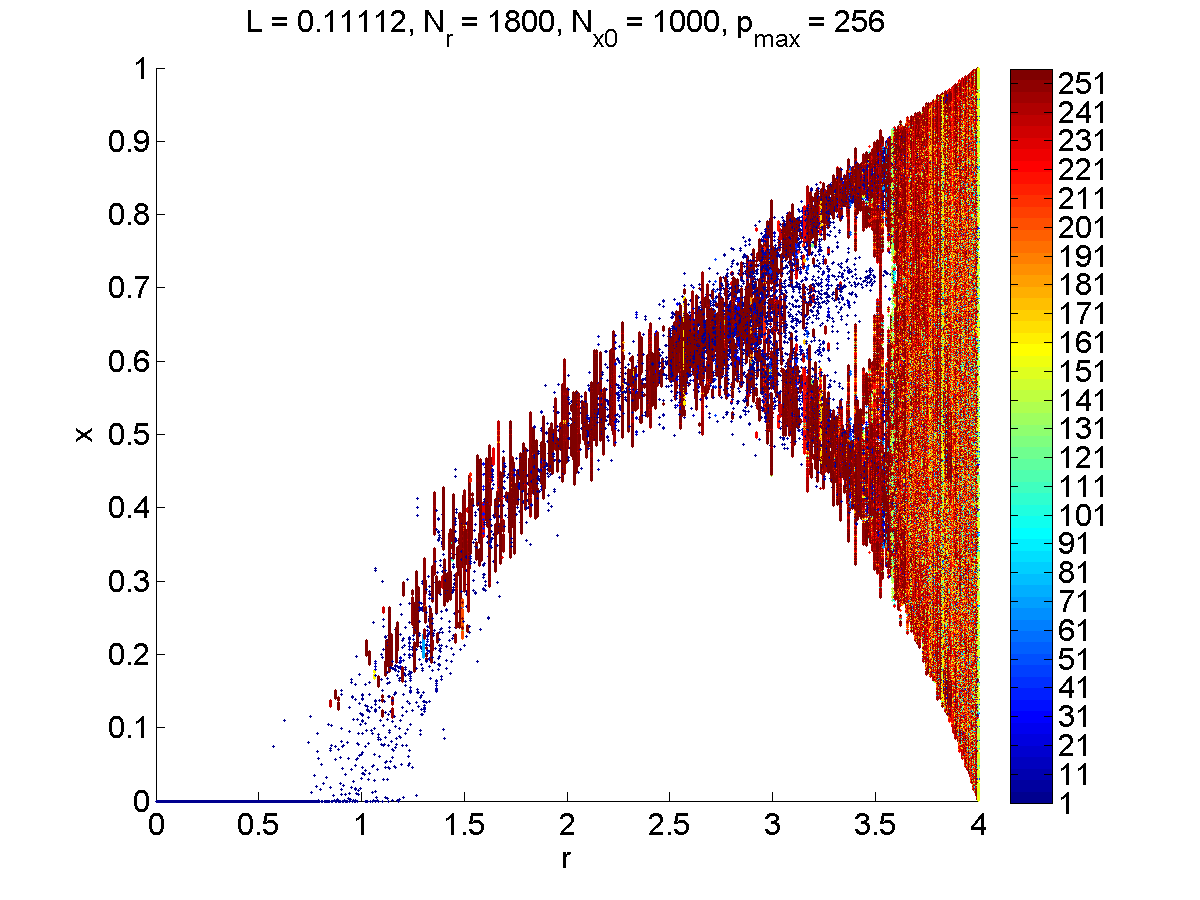
\includegraphics[width=.5\textwidth]{figs/rlog_bif_L_01.png}\hfill
		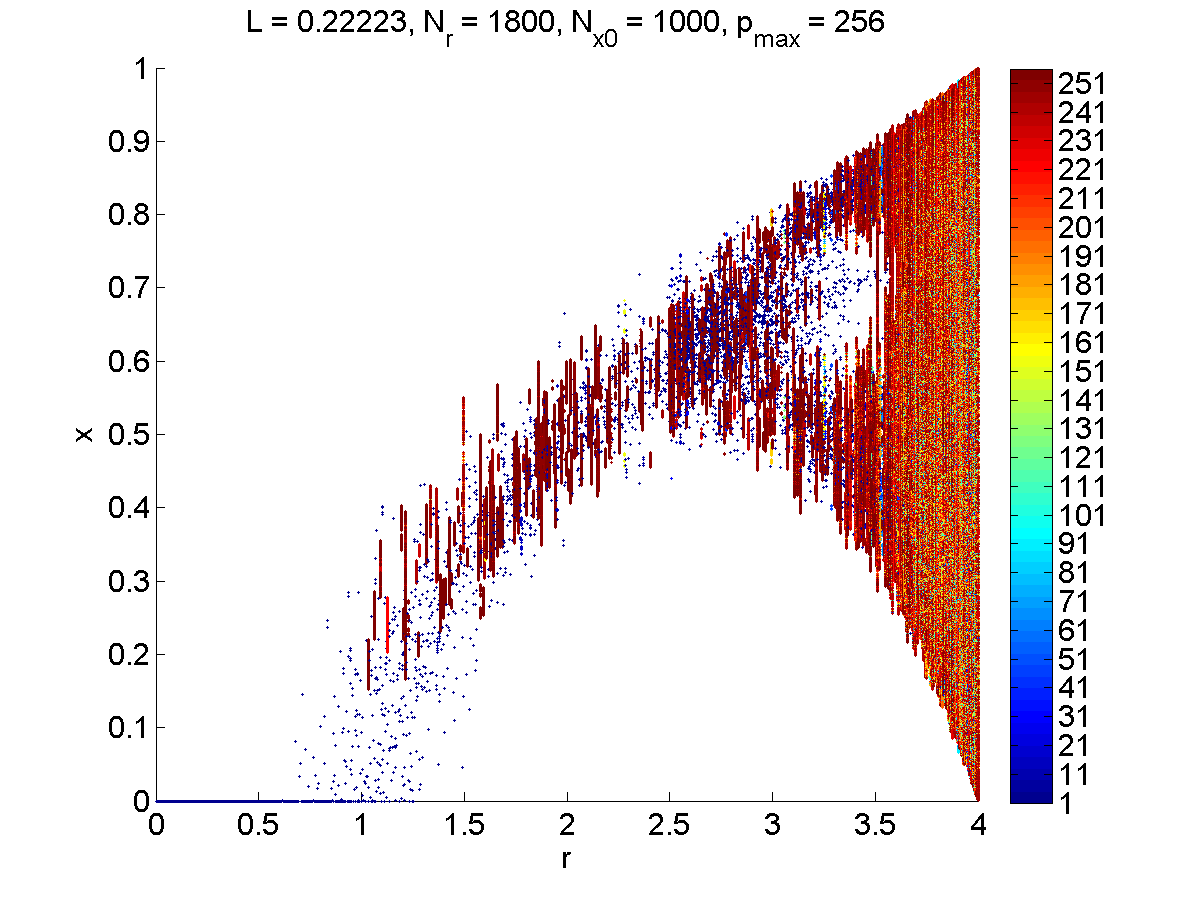
\includegraphics[width=.5\textwidth]{figs/rlog_bif_L_02.png}\\
		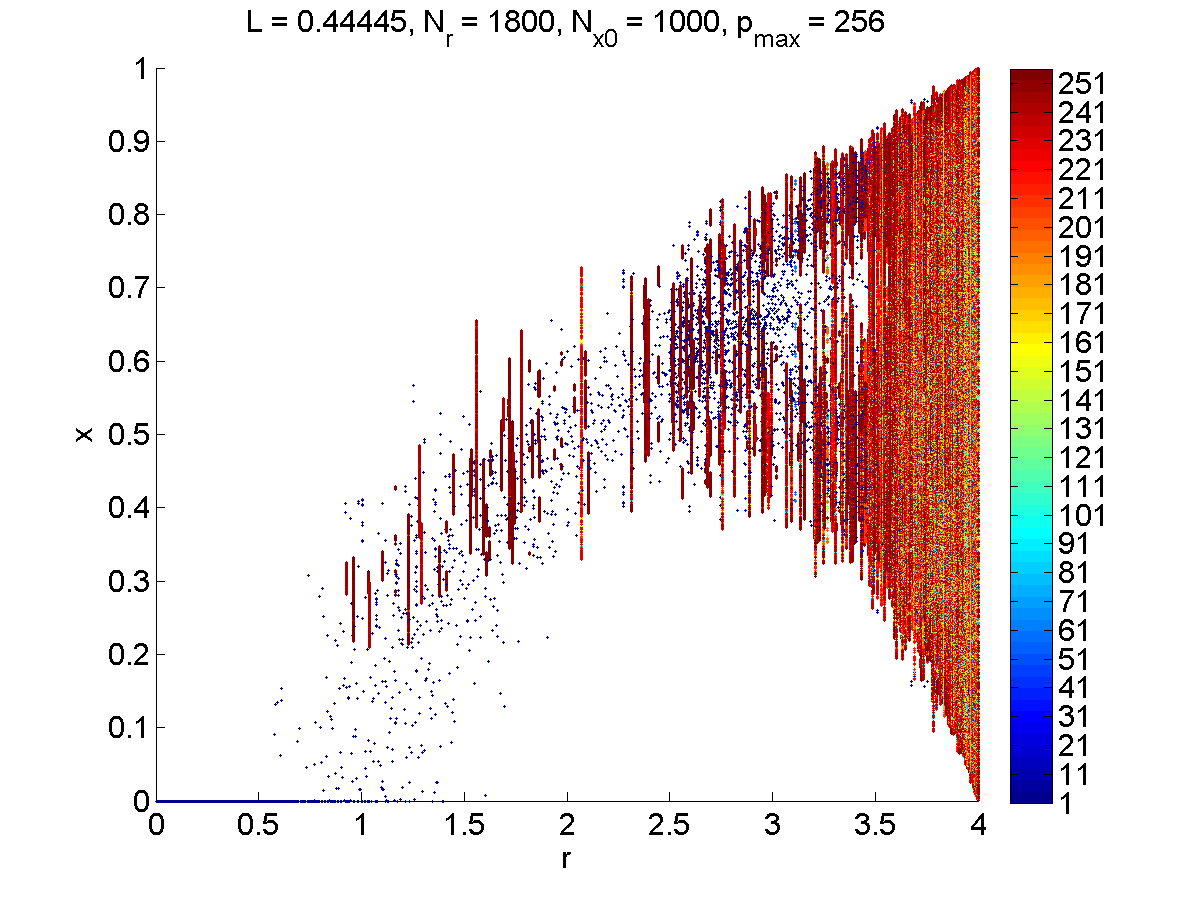
\includegraphics[width=.5\textwidth]{figs/rlog_bif_L_04.png}\hfill
		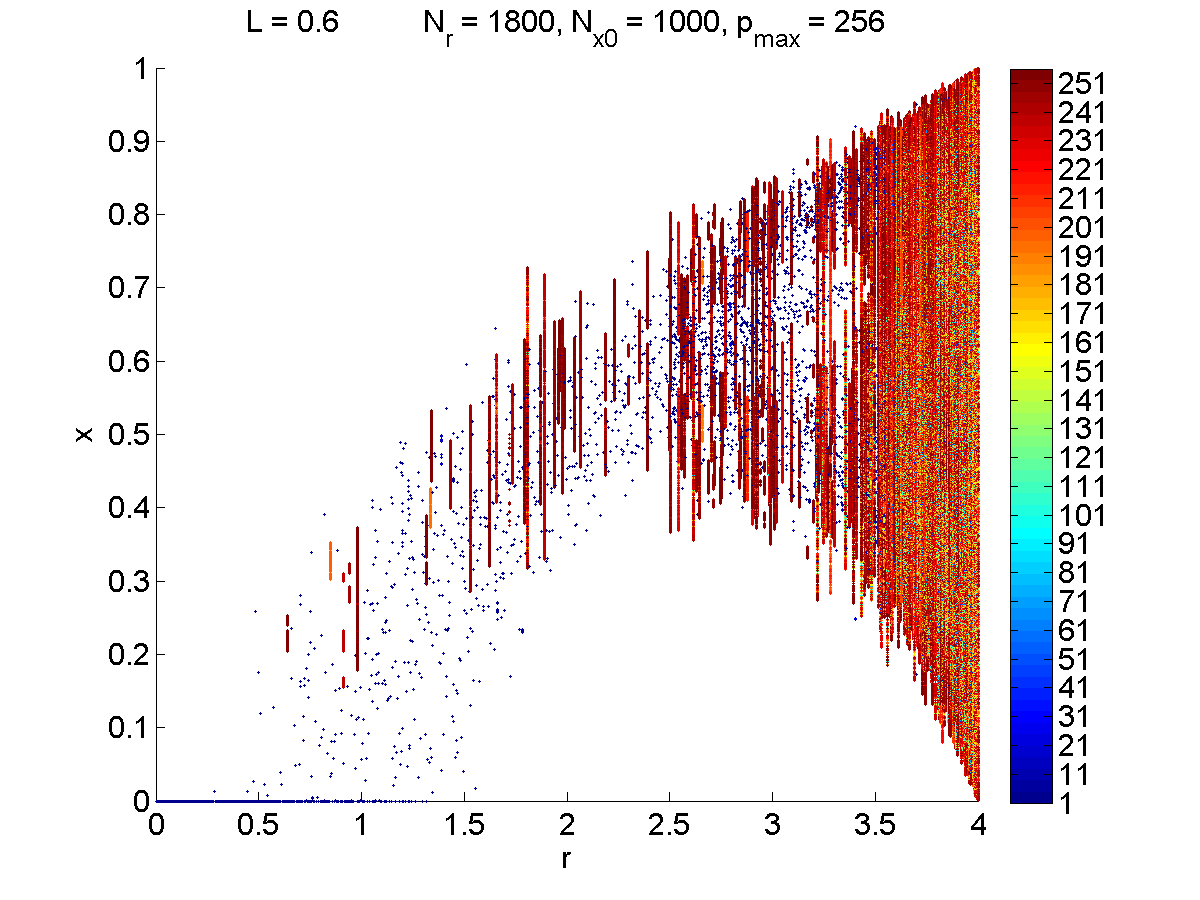
\includegraphics[width=.5\textwidth]{figs/rlog_bif_L_06.png}\\
		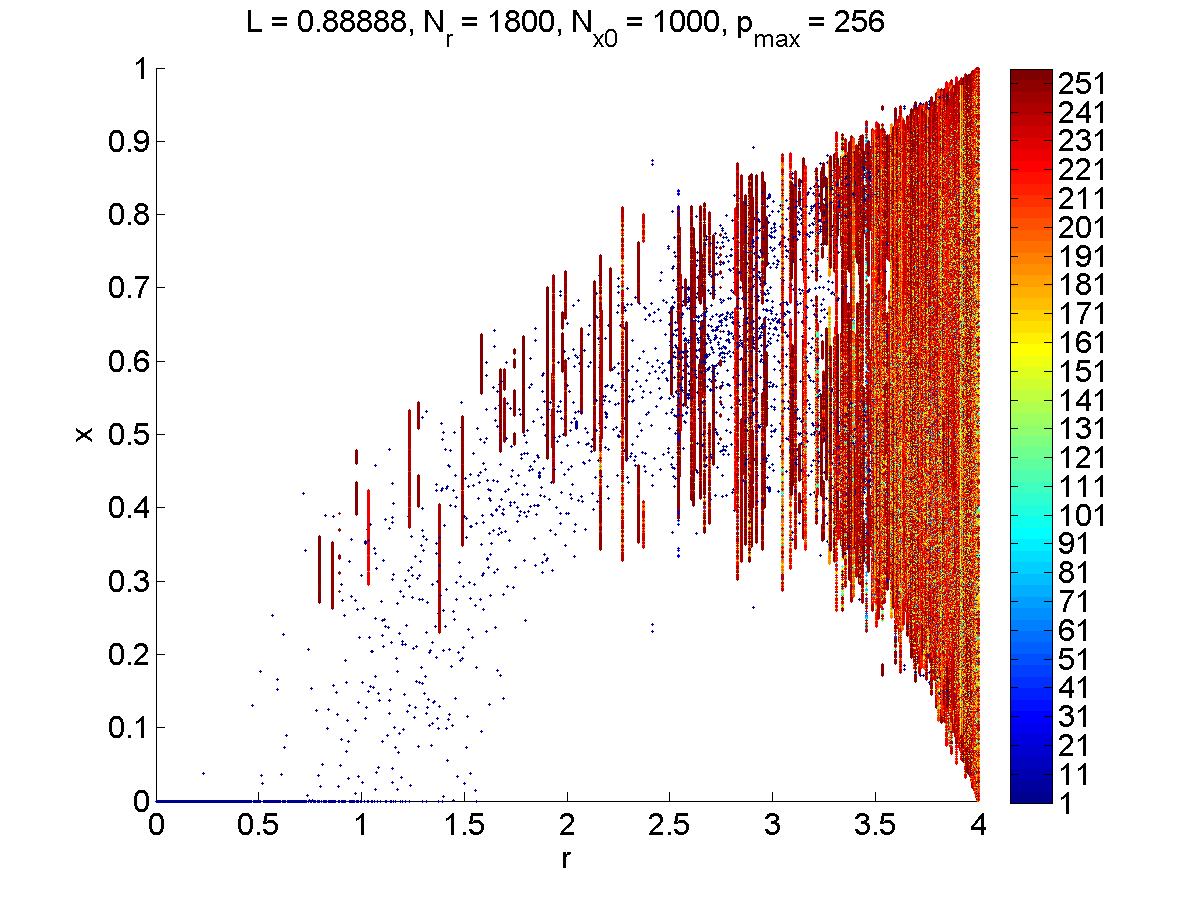
\includegraphics[width=.5\textwidth]{figs/rlog_bif_L_08.png}\hfill
		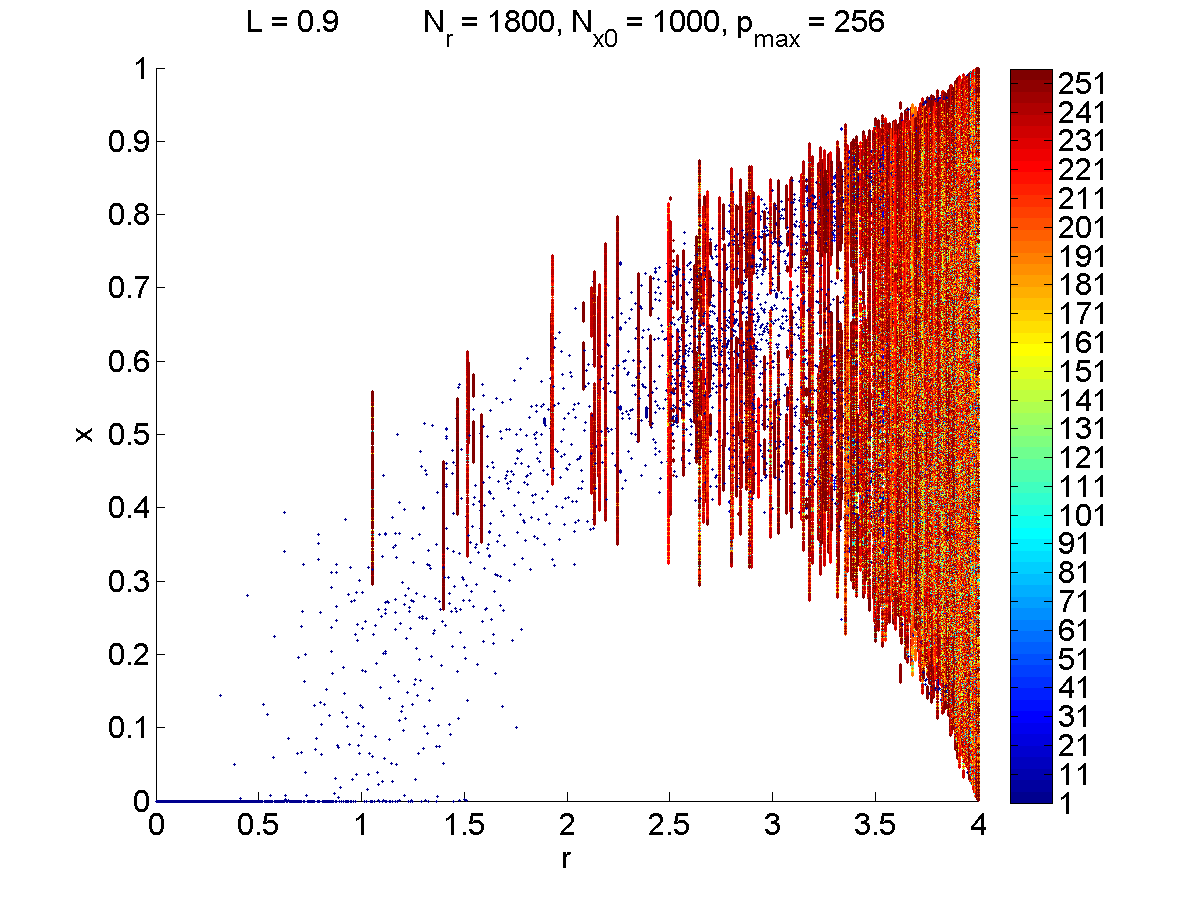
\includegraphics[width=.5\textwidth]{figs/rlog_bif_L_09.png}\\
	\end{center}
\end{figure}

\begin{figure}[H]\linespread{1}
\caption[Bifurcation diagram of the random logistic map, $\sigma=\sigma_{max}$, zoomed
in]{A zoomed in view of Figure~\ref{fig:rlogbif}, where $r \in
  [3,4]$, $\Delta r = 0.001$, $N=100$, the number of initial
  conditions tested is $N_{x_0}$, $L\in \{0.1,0.2,0.4,0.6,0.8,0.9\}$,
  and $\sigma=\sigma_{max}$. Plots are read left to right, and top to
bottom. Number of simulations is 1.8 million. The colorbar shows the color for each period. Orbits up to period 256 were checked.}\label{fig:rlogbif_zoom}
	\begin{center}
		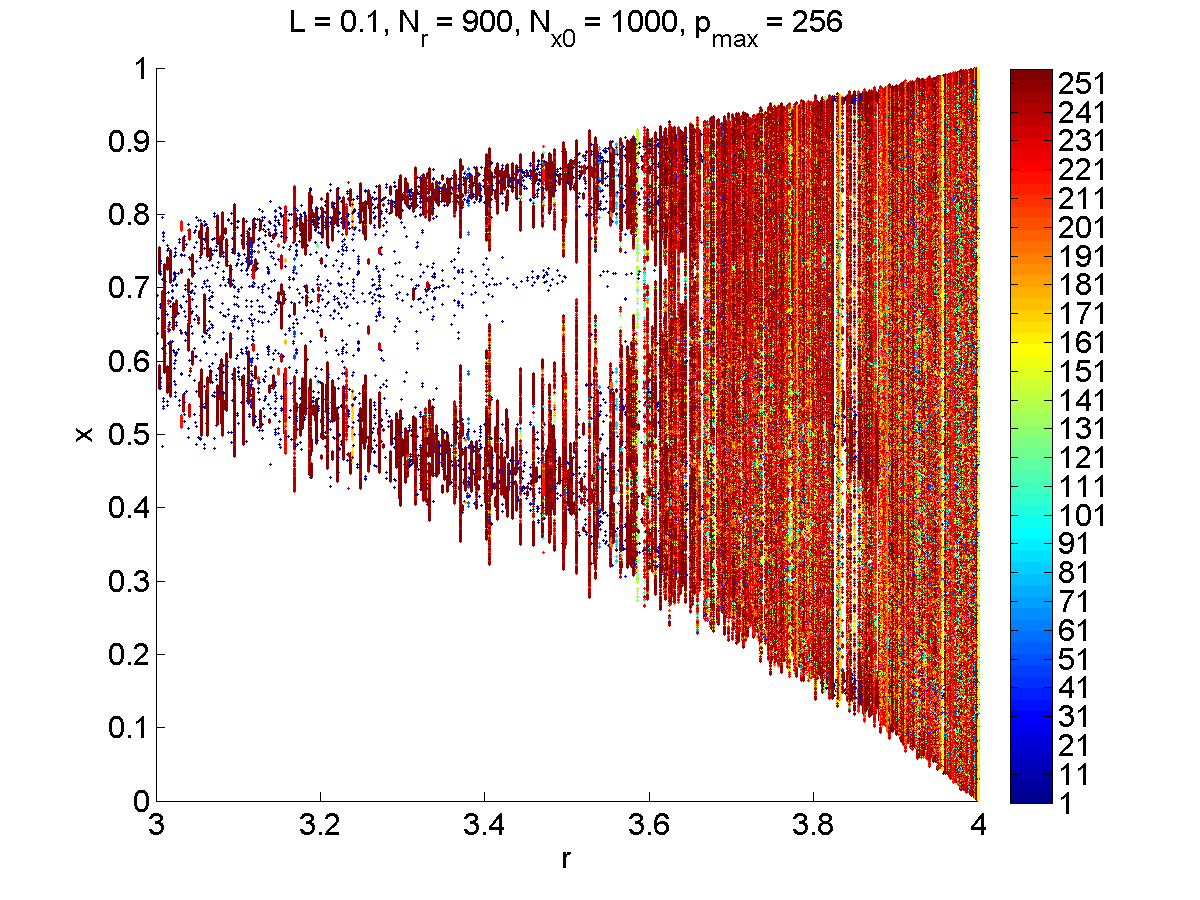
\includegraphics[width=.5\textwidth]{figs/rlog_bif_zoom_L_01.png}\hfill
		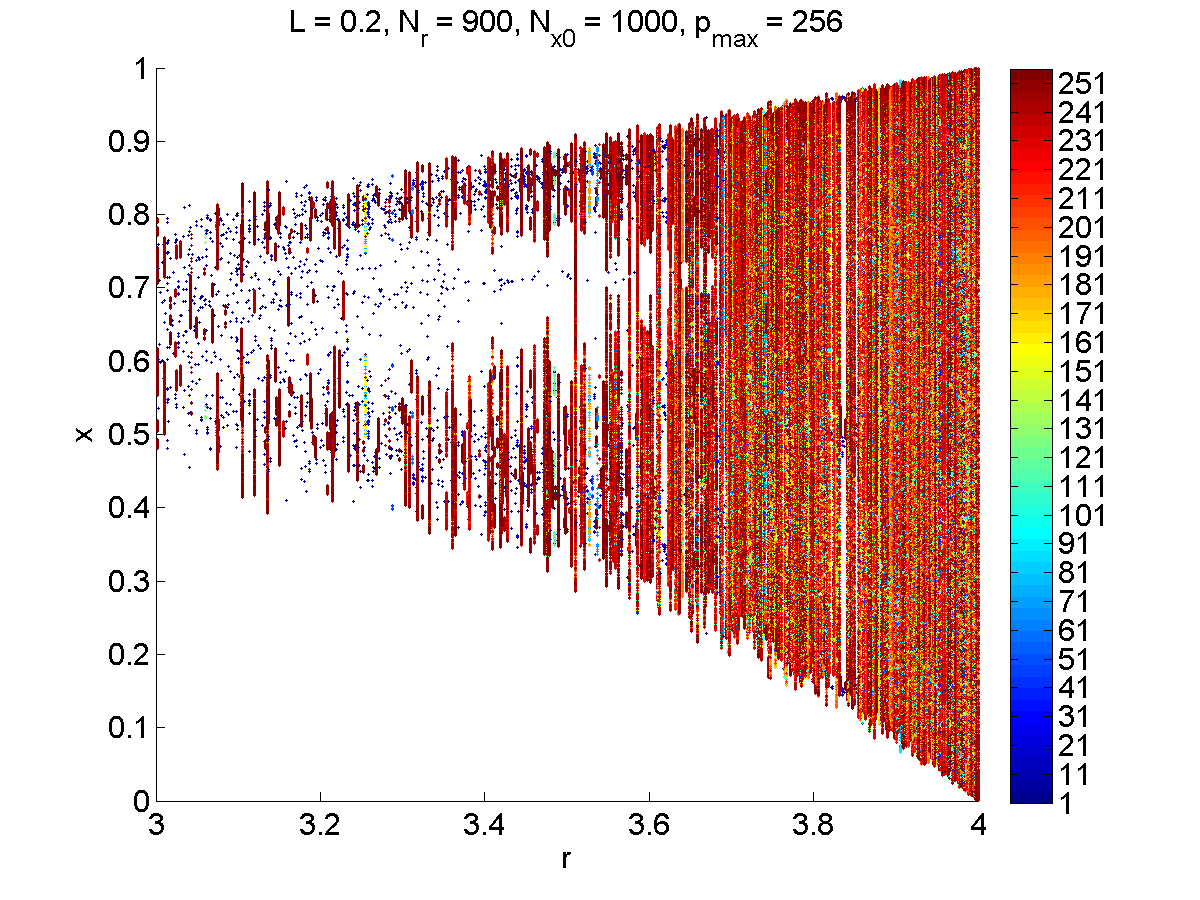
\includegraphics[width=.5\textwidth]{figs/rlog_bif_zoom_L_02.png}\\
		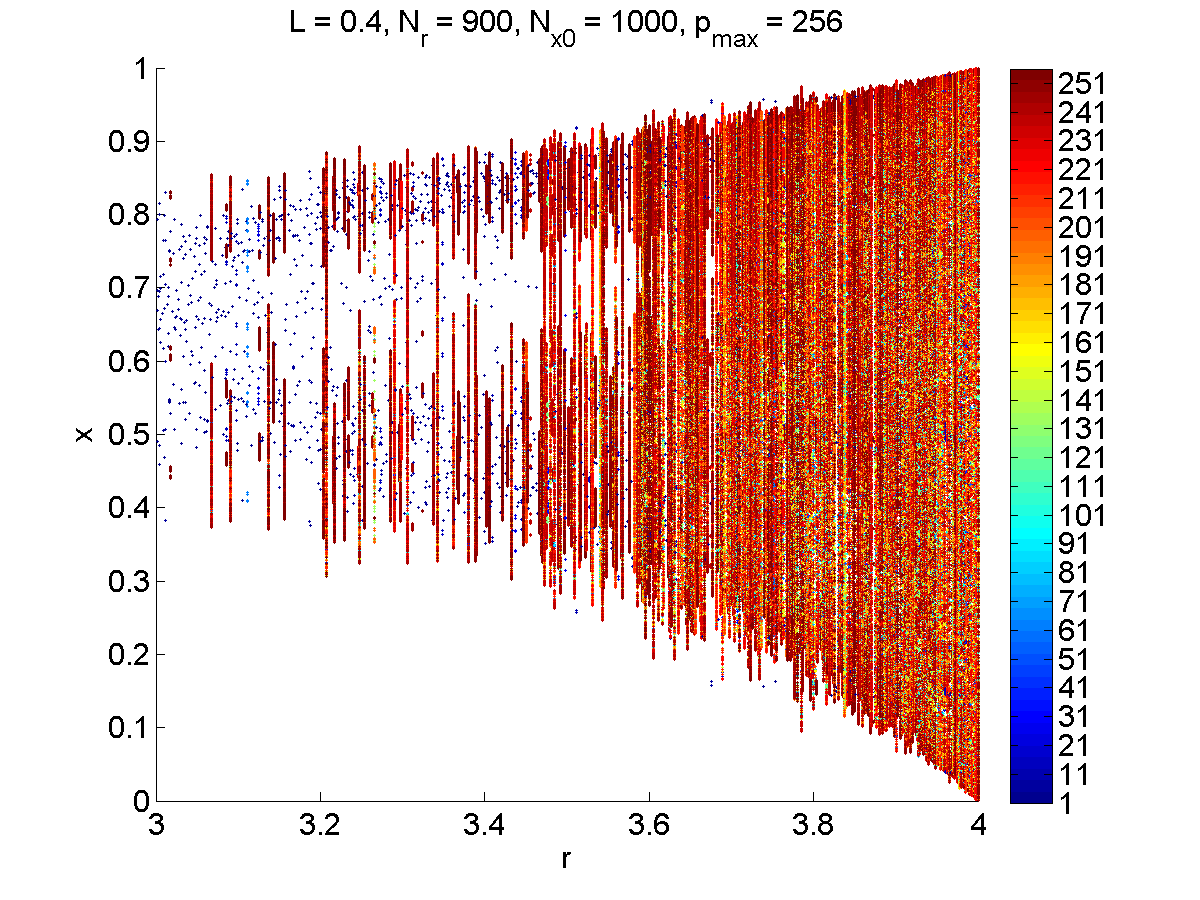
\includegraphics[width=.5\textwidth]{figs/rlog_bif_zoom_L_04.png}\hfill
		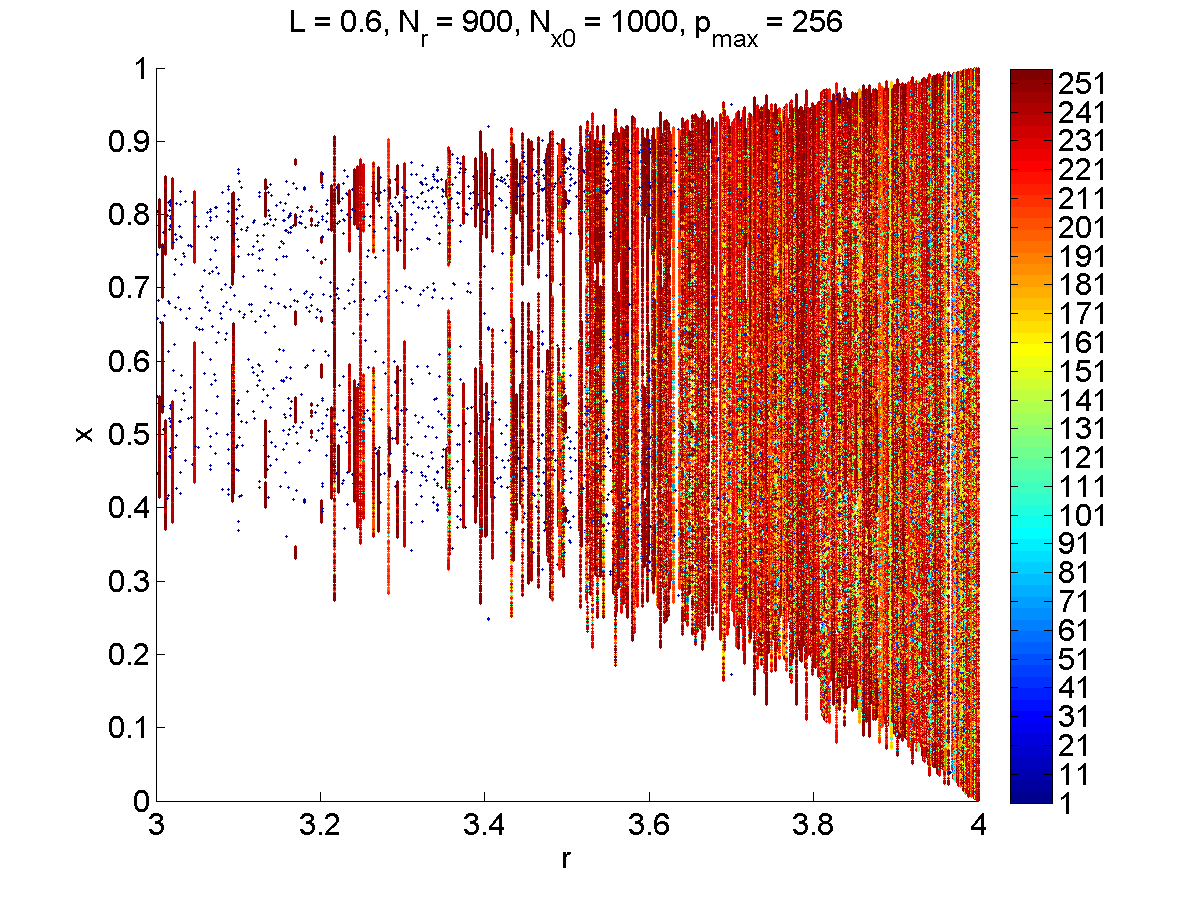
\includegraphics[width=.5\textwidth]{figs/rlog_bif_zoom_L_06.png}\\
		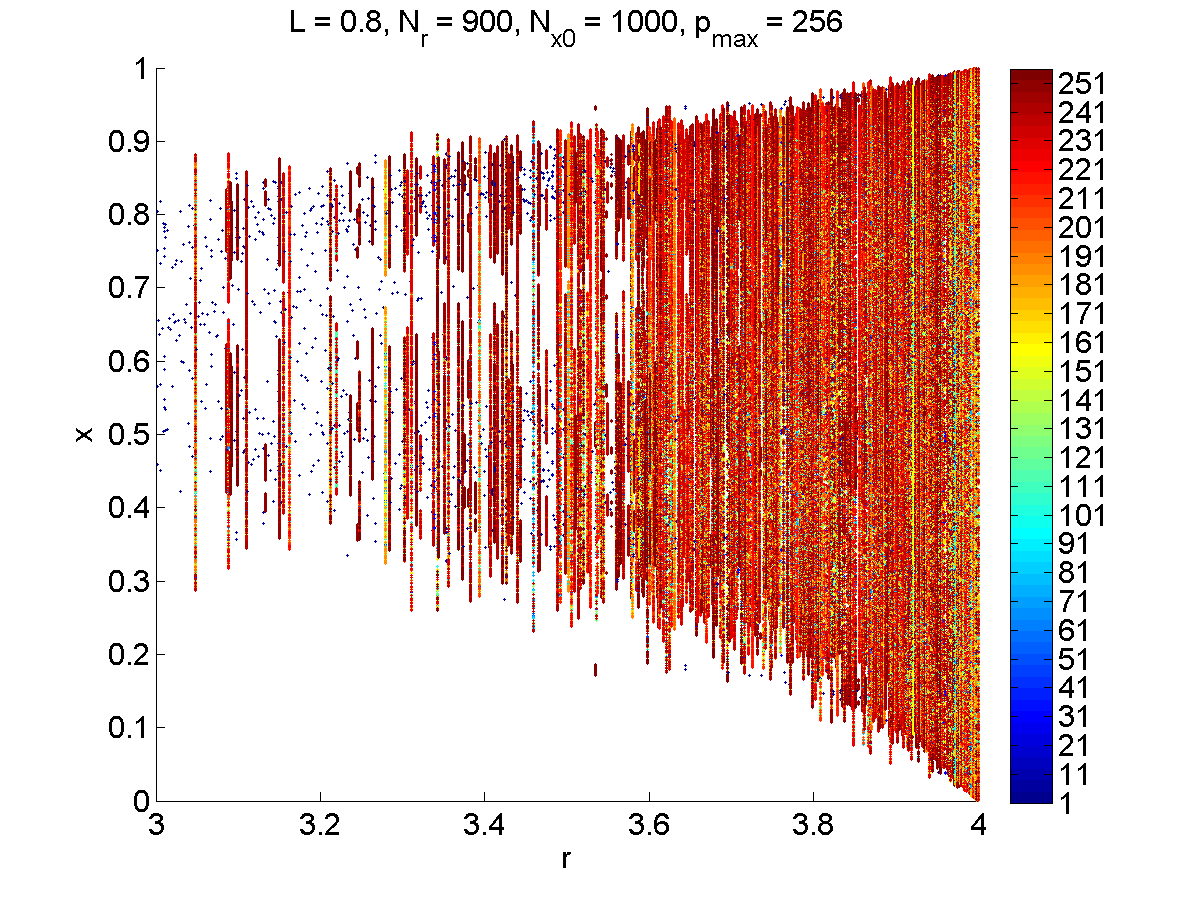
\includegraphics[width=.5\textwidth]{figs/rlog_bif_zoom_L_08.png}\hfill
		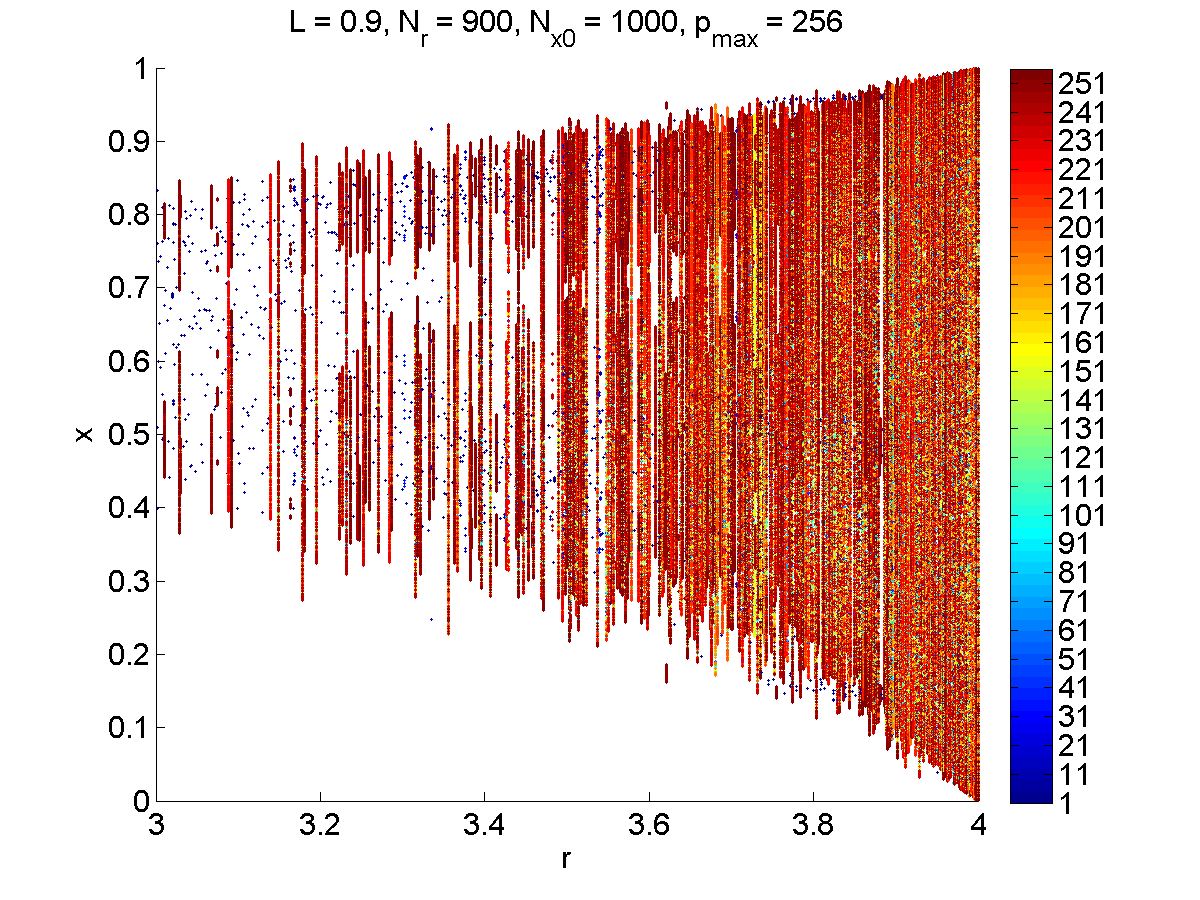
\includegraphics[width=.5\textwidth]{figs/rlog_bif_zoom_L_09.png}\\
	\end{center}
\end{figure}

\begin{figure}[!h]
\caption[Lyapunov exponent in the random logistic map compared to the
deterministic map, $\sigma=\sigma_{max}$]{The Lyapunov exponent for the deterministic
  logistic map (top left) is compared
  to the Lyapunov exponent of the random logistic map for $L \in
  \{0.05,0.1,0.5,0.7,0.9\}$, where $x_0=0.7$ for $r \in [3,4]$, and
  $\sigma$ is chosen to be the maximal value in the interval
  from~(\ref{sigma}). The number of exponents computed was $N_\lambda=10,000$. Plots are read left to right, and top to bottom. }\label{fig:rloglyap2}
\centering
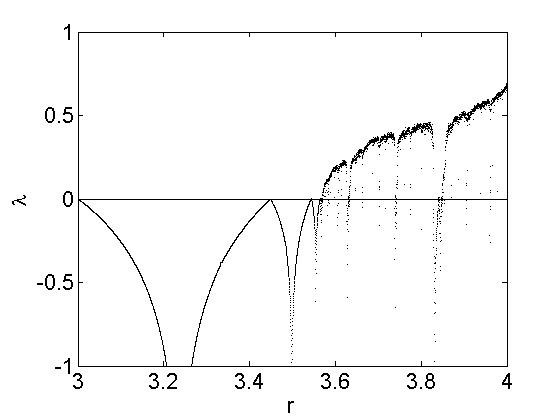
\includegraphics[width=.5\textwidth]{figs/det_log_lyap.png}\hfill
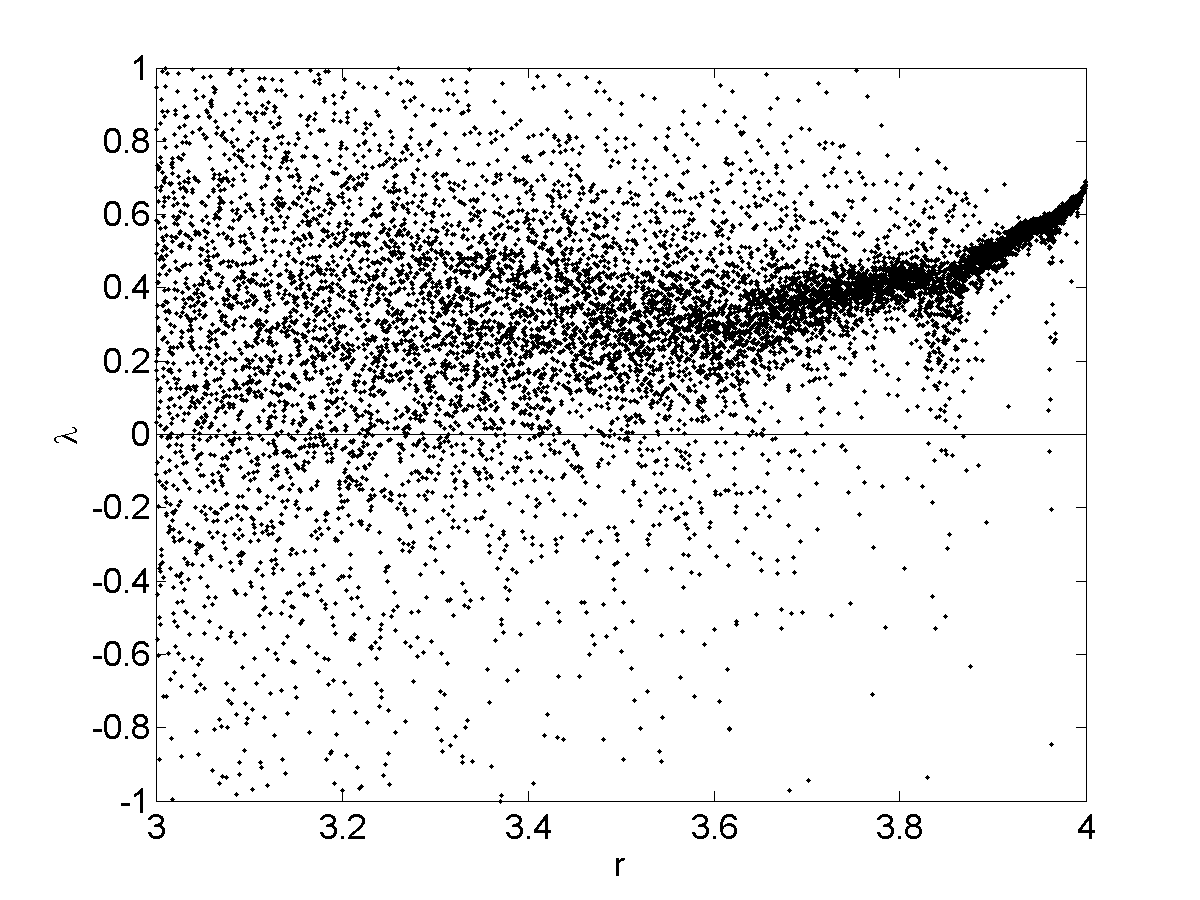
\includegraphics[width=.5\textwidth]{figs/rlog_lyap_L_005.png}\\
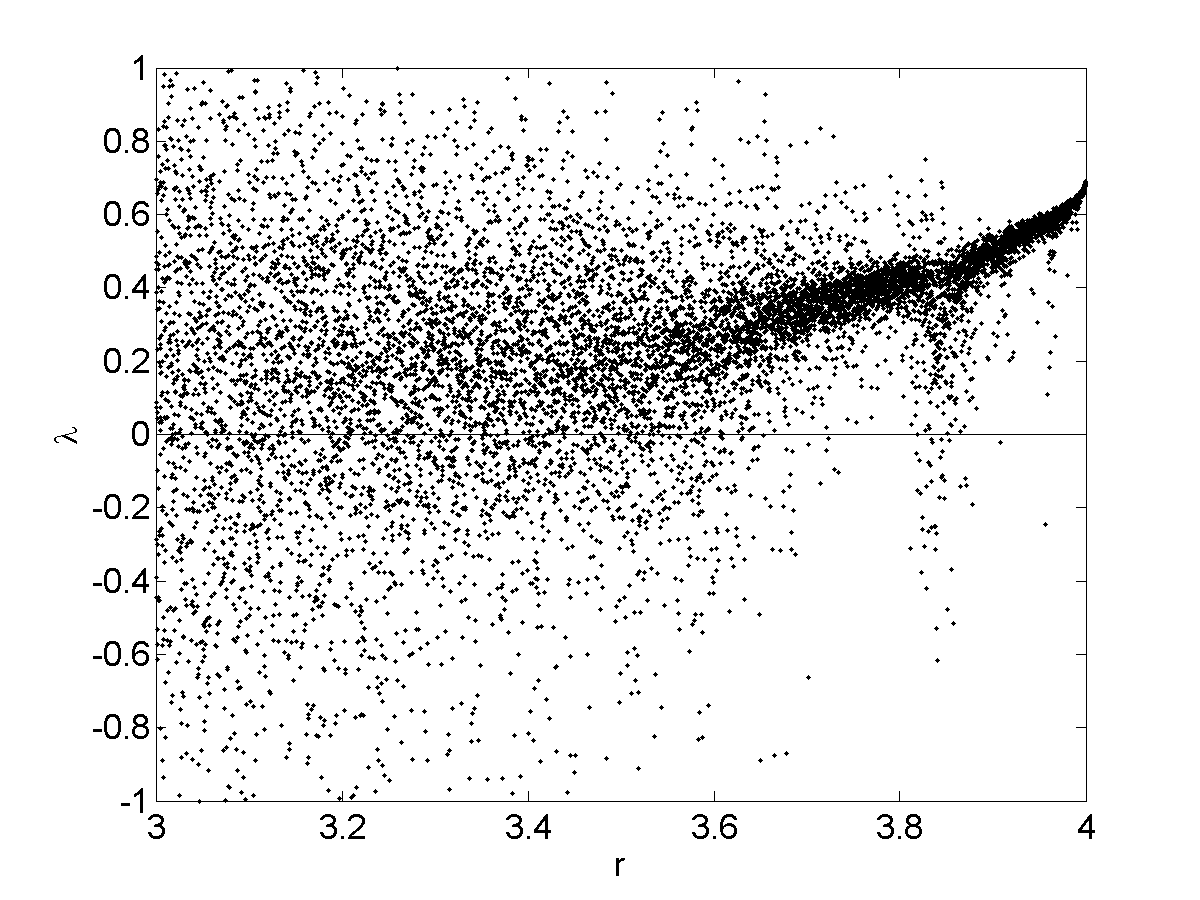
\includegraphics[width=.5\textwidth]{figs/rlog_lyap_L_01.png}\hfill
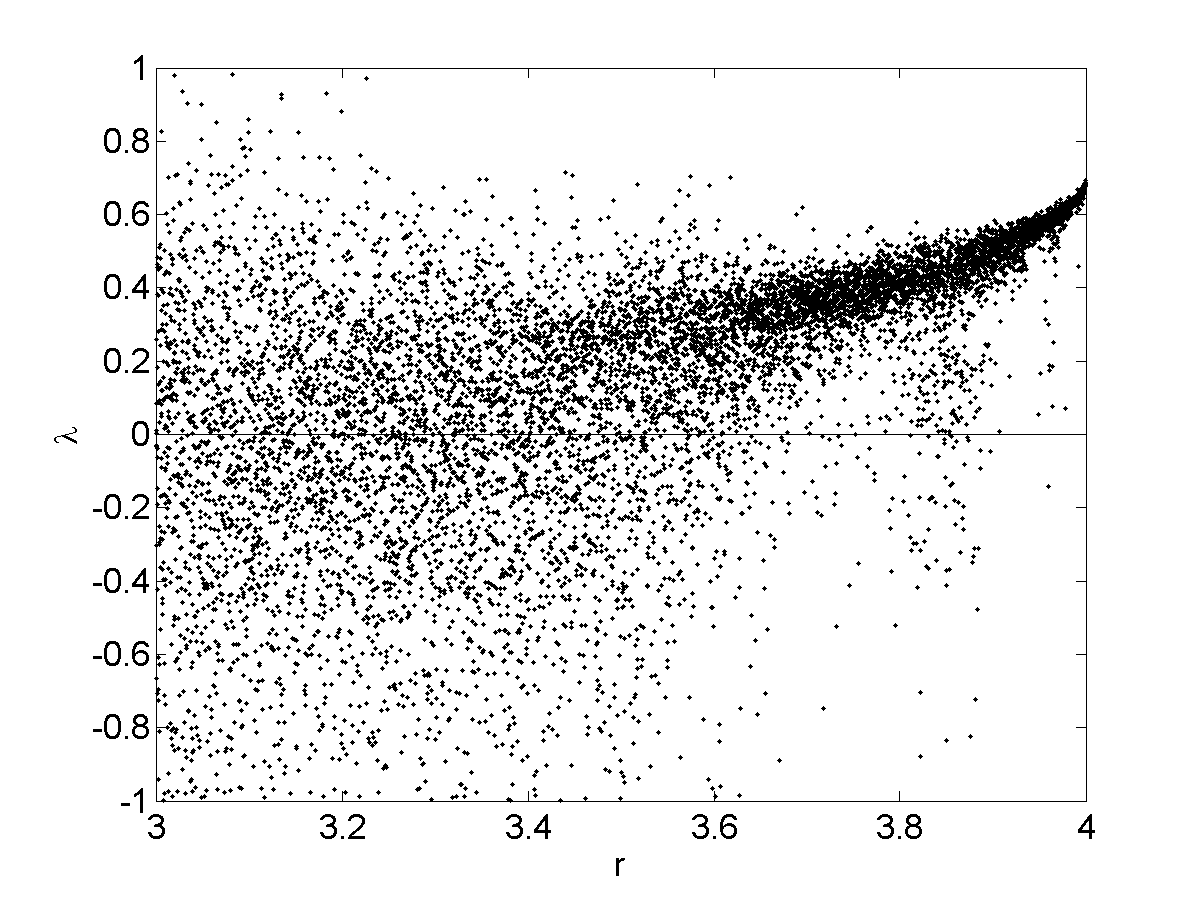
\includegraphics[width=.5\textwidth]{figs/rlog_lyap_L_05.png}\\
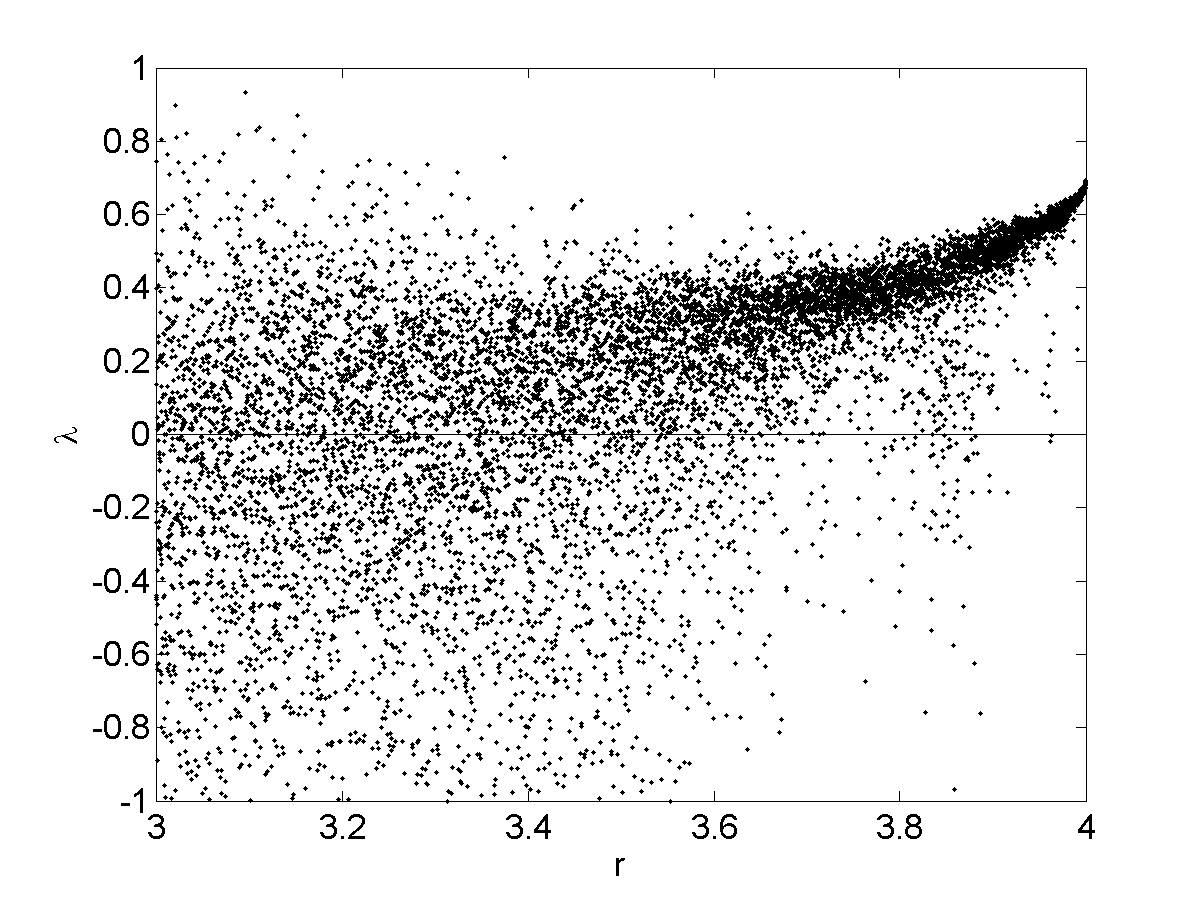
\includegraphics[width=.5\textwidth]{figs/rlog_lyap_L_07.png}\hfill
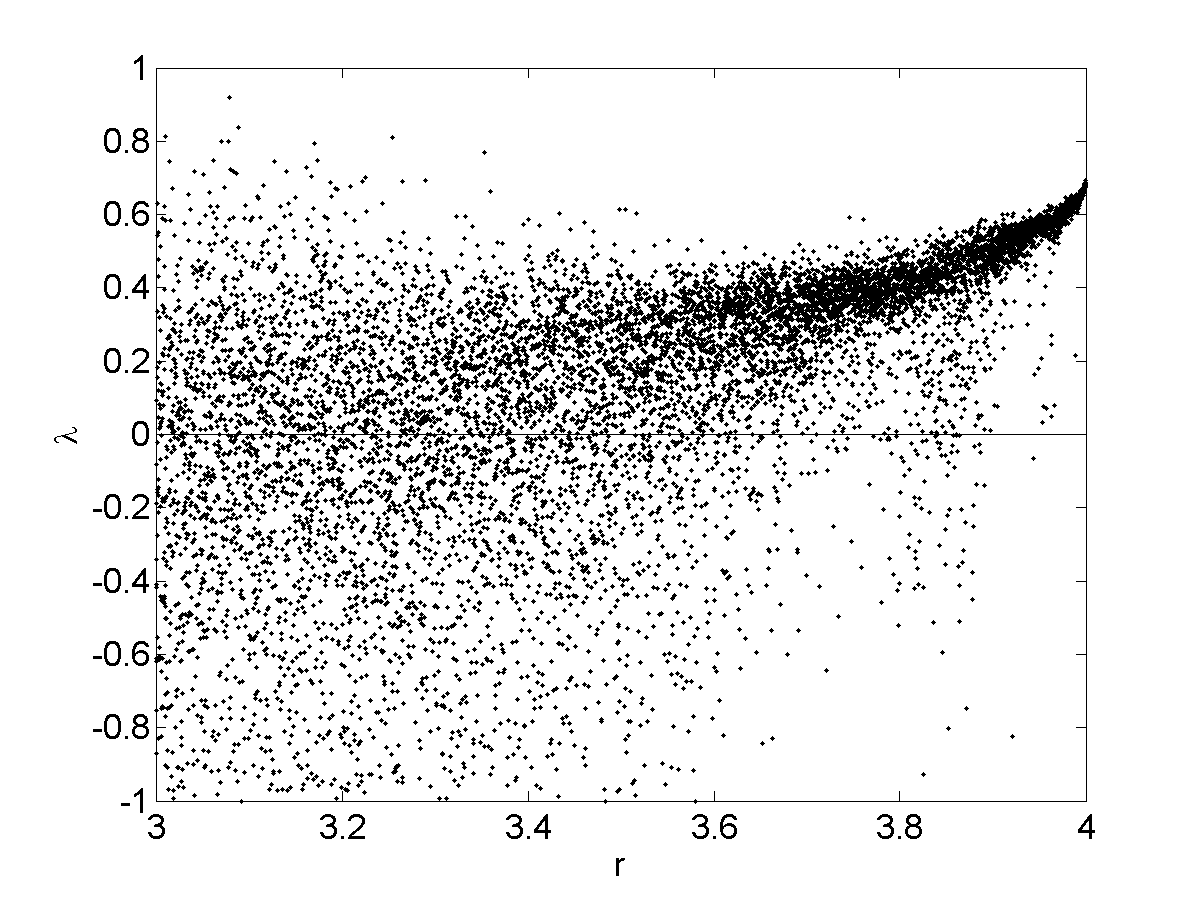
\includegraphics[width=.5\textwidth]{figs/rlog_lyap_L_09.png}\\
\end{figure}

A histogram describing the average fraction of observed period $p$
orbits is shown in Figure~\ref{fig:rloghist}
and~\ref{fig:rloghist2}. The histogram in Figure~\ref{fig:rloghist} implies
that for $r=3.3$, the most commonly observed stable orbit is period 2, and the
distribution of periodic orbits may follow the exponential
distribution. This figure corresponds with the newly stabilized region
of the logistic map. Figure~\ref{fig:rloghist2} scans the distribution
of period for a smaller value of $r=1.2$. Here, the most dominant
period is 1, and the distribution still resembles the exponential. The distribution of period for any given $(r,L)$ pair
offers insight on the type of orbits that the random process solicits.

The histograms were generated by testing 10 random initial conditions $x_0$ 500 times
each, resulting in 5,000 total simulations. Each time any given $x_0$
was tested, a new set of random Fourier modes $\hat{\xi}_n$ were drawn
from either a uniform or normal distribution. After iterating the random
map 1,000 for some $r$ and this set of Fourier modes, an orbit was denoted period $p$ if $x_p = x_{n+p}$ within a
tolerance of $\epsilon = 10^{-6}$. Periodicity was checked up to
$p_{max}=100$. The histograms count unique periodic orbits, so if two
or more initial conditions under the same random process converged to the same periodic orbit, only
one was counted. 

\begin{figure}[H]\linespread{1}
\caption[Average number of period $p$ orbits for the random logistic
map, $\sigma=\sigma_{max}$ and $r=3.3$]{Average number of period $p$ orbits for the random logistic
map, where 5000 simulations are plotted. The error bars indicate
the standard error of the calculation of the mean. In all plots,
$r=1.2$ and $\sigma=\sigma_{max}$. For $(L,N,\sigma)$,
we have $(0.025, 400, 0.0087808)$ (left), $(0.05, 200, 0.012418)$
(middle), and $(0.1, 100, 0.017565)$ (right).}\label{fig:rloghist}
	\begin{center}
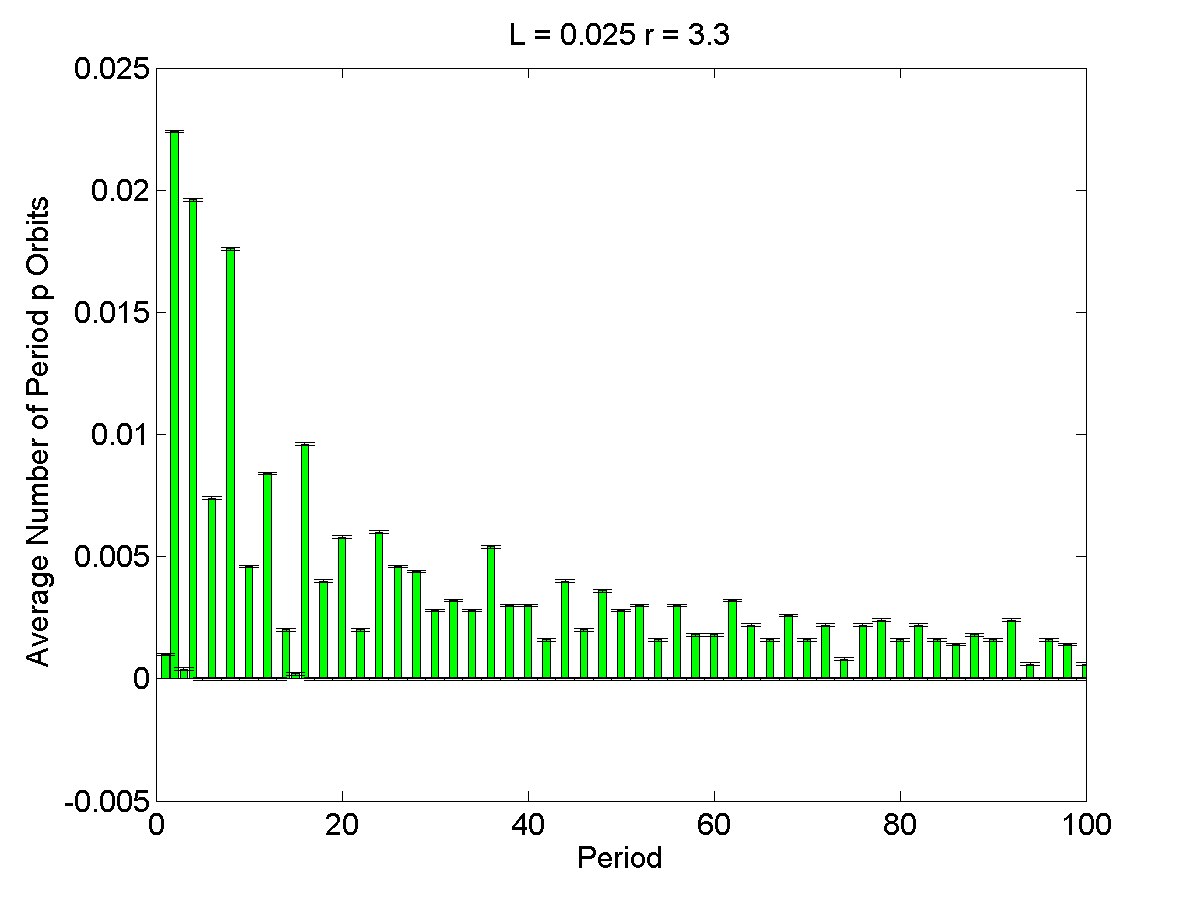
\includegraphics[width=.33\textwidth]{figs/rlog_hist_L_0025_r_33_s_00087808_a_96372e-07_sims_5000.png}\hfill		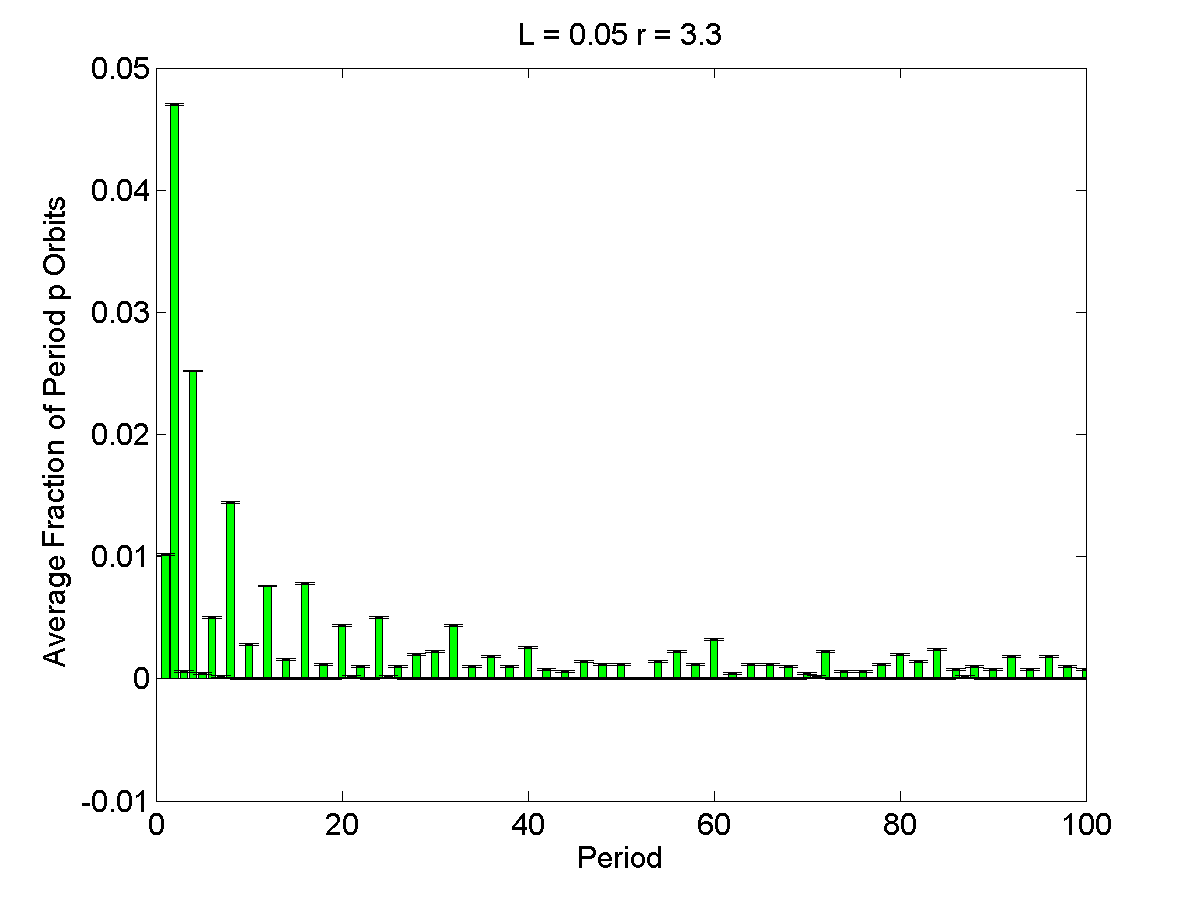
\includegraphics[width=.33\textwidth]{figs/rlog_hist_L_005_r_33_s_0012418_a_38546e-06_sims_5000.png}\hfill
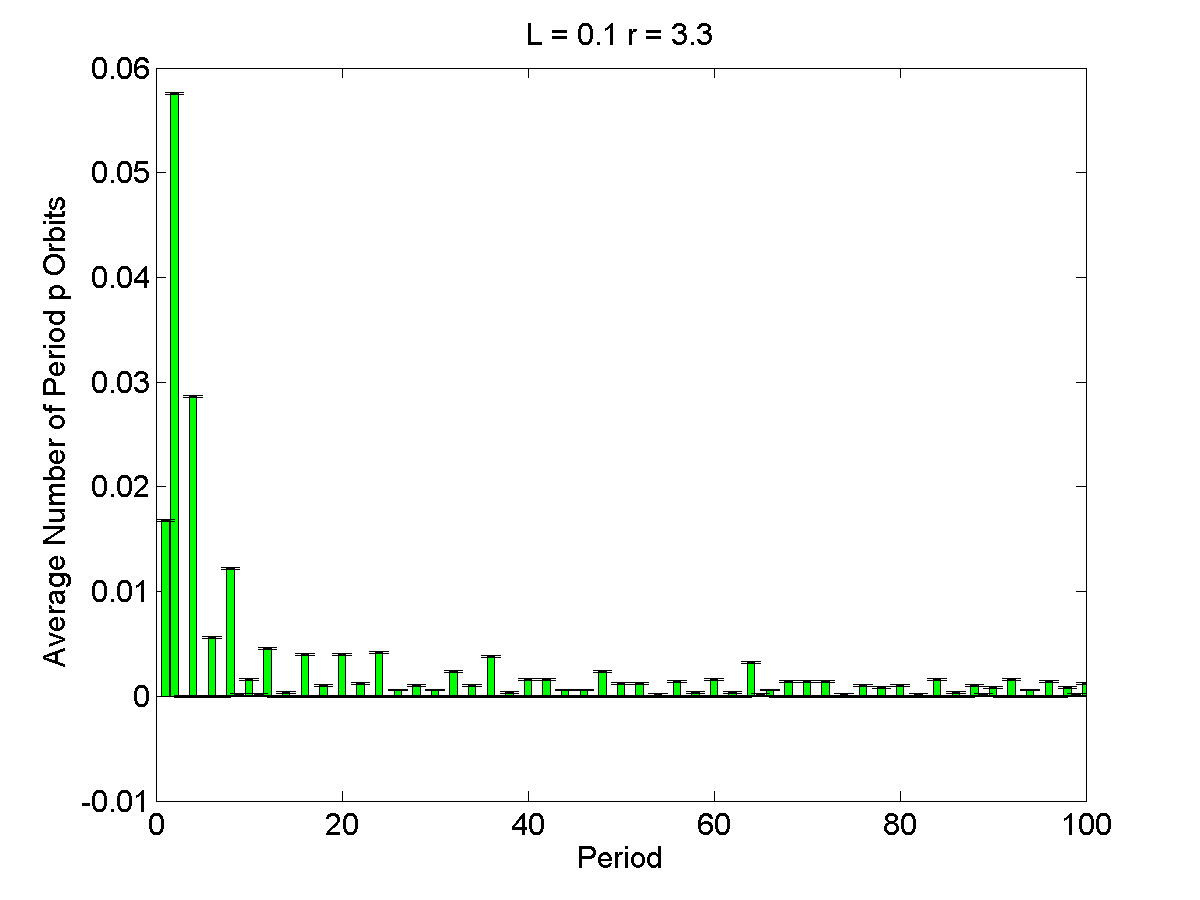
\includegraphics[width=.33\textwidth]{figs/rlog_hist_L_01_r_33_s_0017565_a_15414e-05_sims_5000.png}
	\end{center}
\end{figure}

\begin{figure}[H]\linespread{1}
\caption[Average number of period $p$ orbits for the random logistic
map, $\sigma=\sigma_{max}$ and $r=1.2$]{Average number of period $p$ orbits for the random logistic
map, where 5000 simulations are plotted. The error bars indicate
the standard error of the calculation of the mean. In all plots,
$r=1.2$ and $\sigma=\sigma_{max}$. For $(L,N,\sigma)$,
we have $(0.05, 200, 0.07772)$ (left), $(0.1, 100, 0.10993)$
(middle), and $(0.2, 100, 0.15556)$ (right).}\label{fig:rloghist2}
	\begin{center}	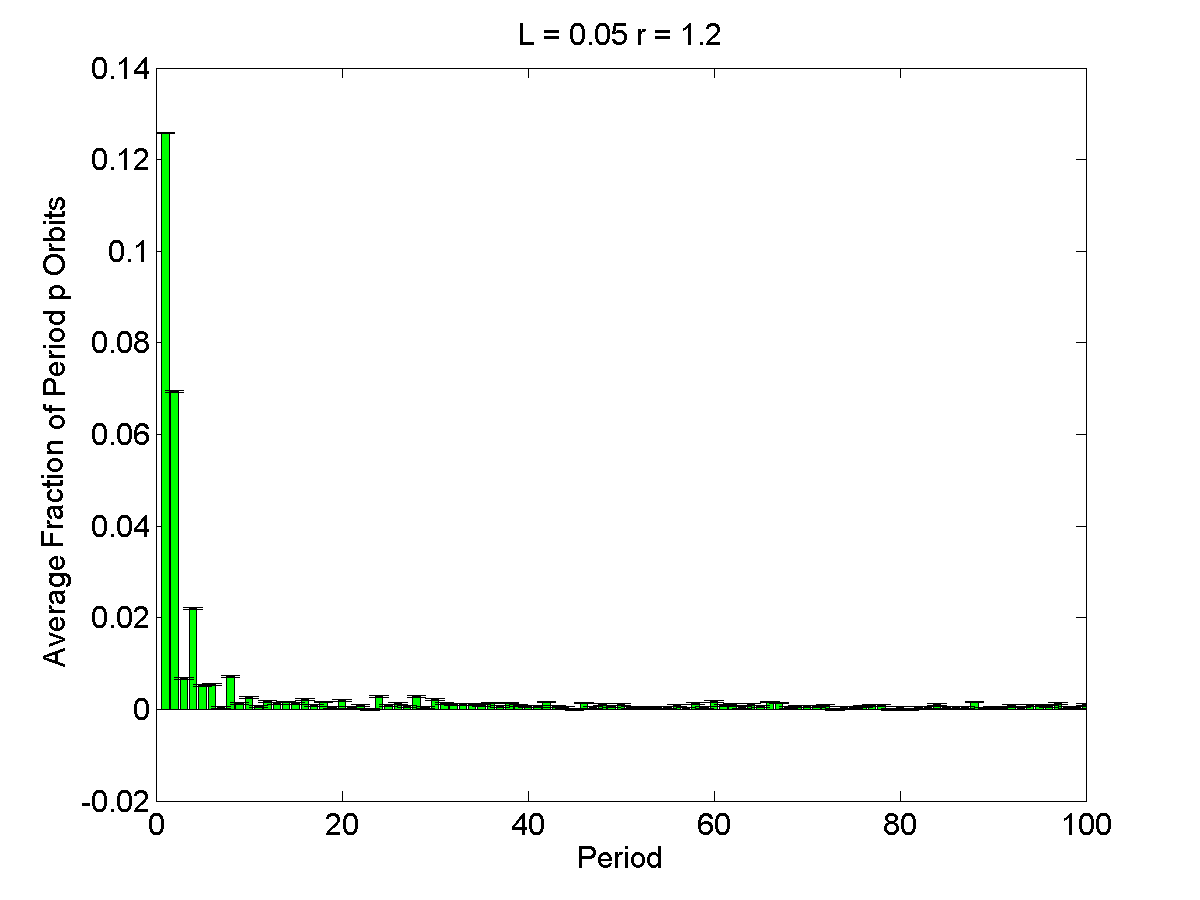
\includegraphics[width=.33\textwidth]{figs/rlog_hist_L_005_r_12_s_007772_a_000015098_sims_5000.png}\hfill
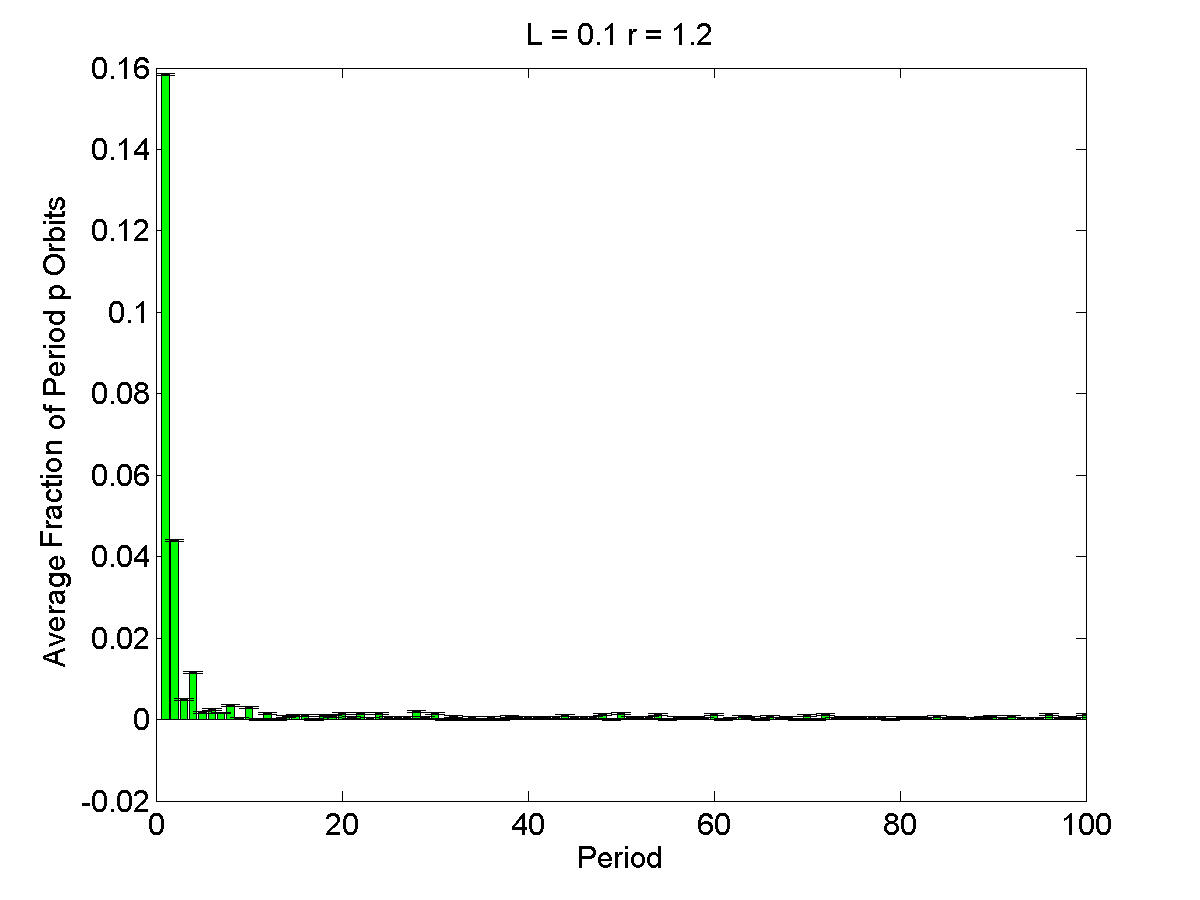
\includegraphics[width=.33\textwidth]{figs/rlog_hist_L_01_r_12_s_010993_a_000060373_sims_5000.png}\hfill	
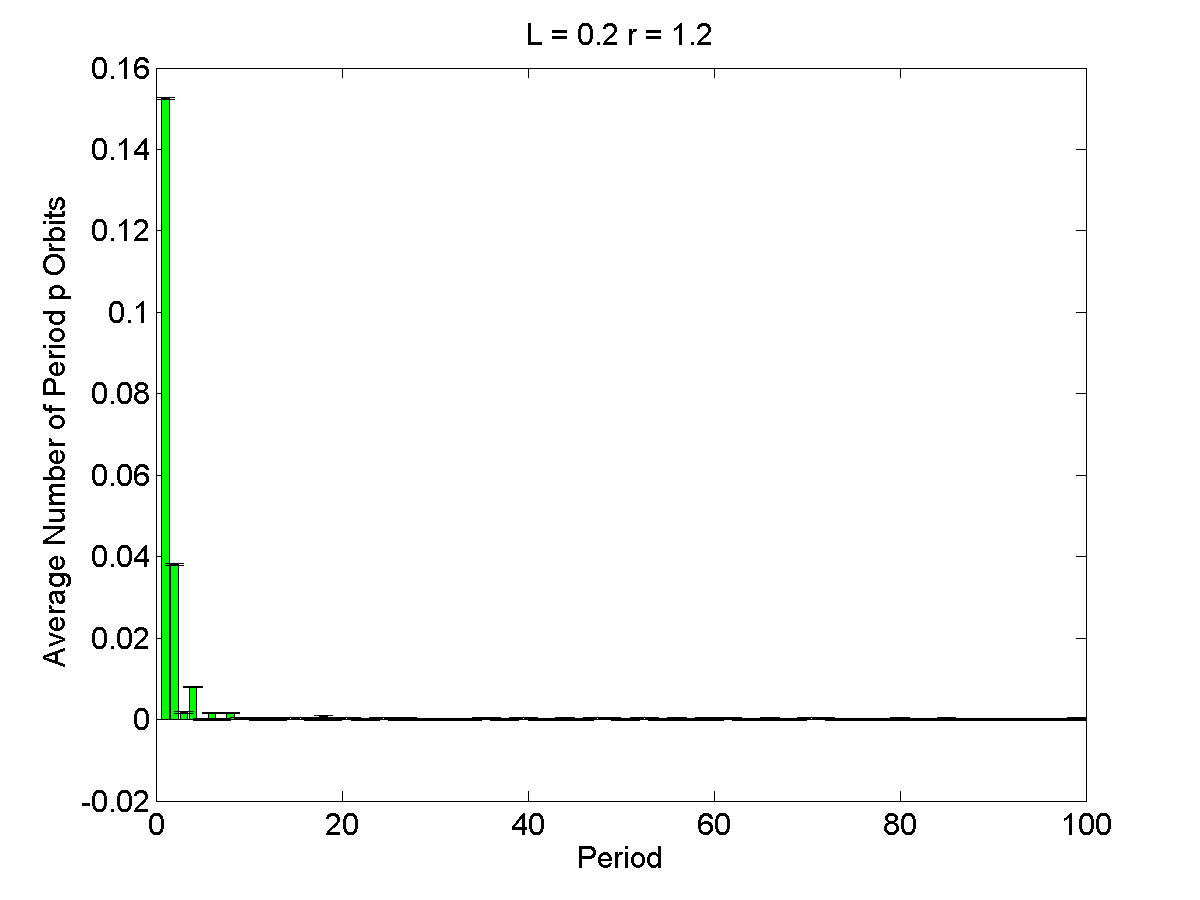
\includegraphics[width=.33\textwidth]{figs/rlog_hist_L_02_r_12_s_015556_a_00024119_sims_5000.png}
	\end{center}
\end{figure}

Figure~\ref{fig:rlogbif_hs} and Figure~\ref{fig:rloglyap2_hs}
demonstrate results from simulating the random logistic map where the
variance $\sigma$ of $\xi(x)$ is chosen to be half of the maximal
value from~(\ref{sigma}). Not surprisingly, the stable low period
orbits for $r \in [3,4]$ endure even
when the noise is restricted. Further, it appears the density of
stable orbits for $r<3$ diminishes as $L$ is increased. Additionally,
there are fewer stable high period orbits when $\sigma$ is small.

The positive Lyapunov exponents of the randomized logistic
map for the case where $\sigma$ is small in
Figure~\ref{fig:rloglyap2_hs} implies that even a halved standard
deviation will incur chaotic behavior. The negative spike around
$r=3.8$, which corresponds to an island of stability in the
deterministic map, is more prominent when $\sigma$ is small than when large. Between
Figure~\ref{fig:rloglyap2} and Figure~\ref{fig:rloglyap2_hs}, it
appears that decreasing $\sigma$ causes the plot of Lyapunov exponents
of the random map to fall more in line with the plot for the
deterministic map. There are fewer positive exponents in
Figure~\ref{fig:rloglyap2_hs} than in Figure~\ref{fig:rloglyap2}, and
remnants of other islands of stability from the deterministic map
appear in the plots of the random map (e.g. $r \approx 3.95$).

\begin{figure}[H]\linespread{1}
\caption[Bifurcation diagram of the random logistic map, $\sigma=\frac{1}{2}\sigma_{max}$]{Bifurcation diagram of the random
logistic map, where $r \in [0,4]$, $\Delta r = 0.002$, $N=100$, the
number of initial conditions tested is $N_{x_0}$, $L\in
\{0.1,0.2,0.4,0.6,0.8,0.9\}$, and $\sigma$ is chosen to be half of the maximal
value in the interval from~(\ref{sigma}). Plots are read left to right, and top to
bottom. Number of simulations is 1.8 million. The colorbar shows the color for each period. Orbits up to period 256 were checked.}\label{fig:rlogbif_hs}
	\begin{center}
		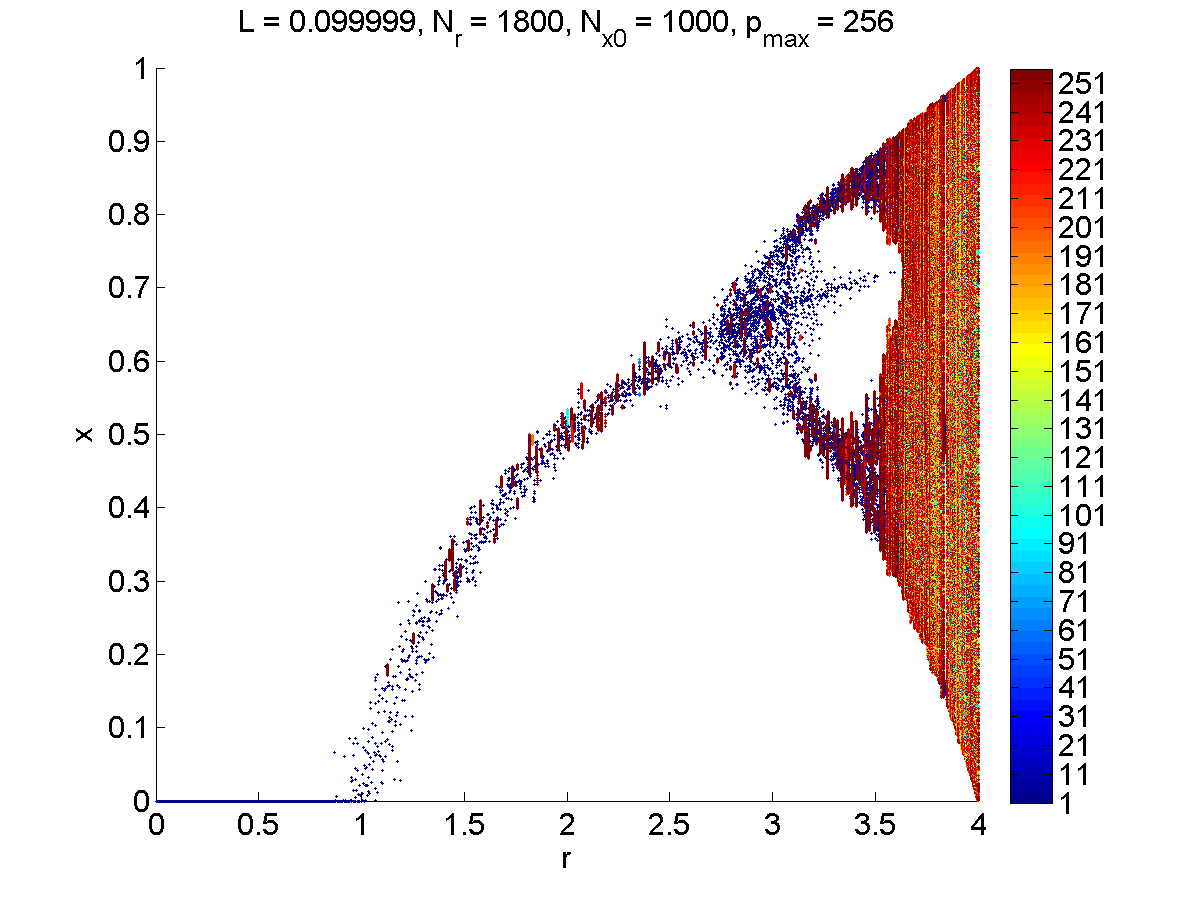
\includegraphics[width=.5\textwidth]{figs/rlog_bif_halfs_L_01.png}\hfill
		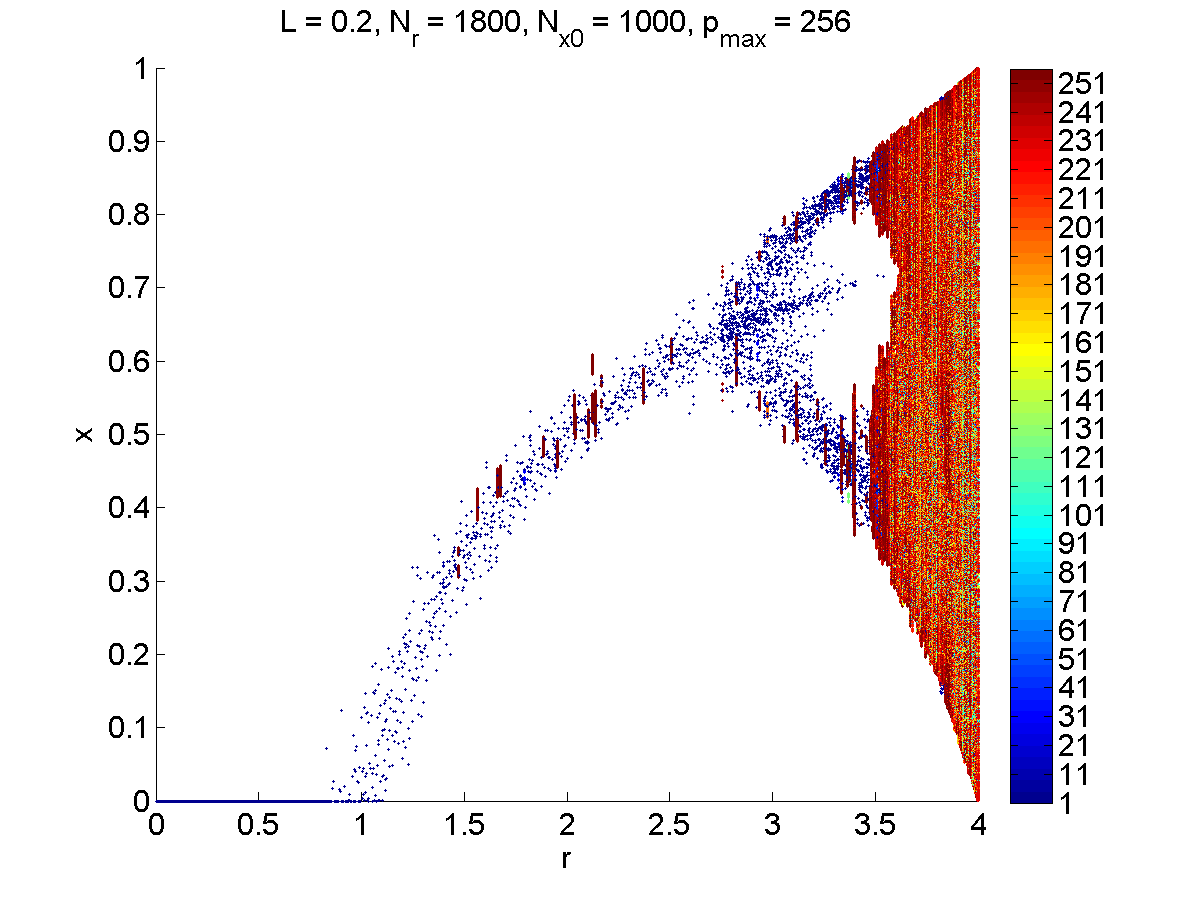
\includegraphics[width=.5\textwidth]{figs/rlog_bif_halfs_L_02.png}\\
		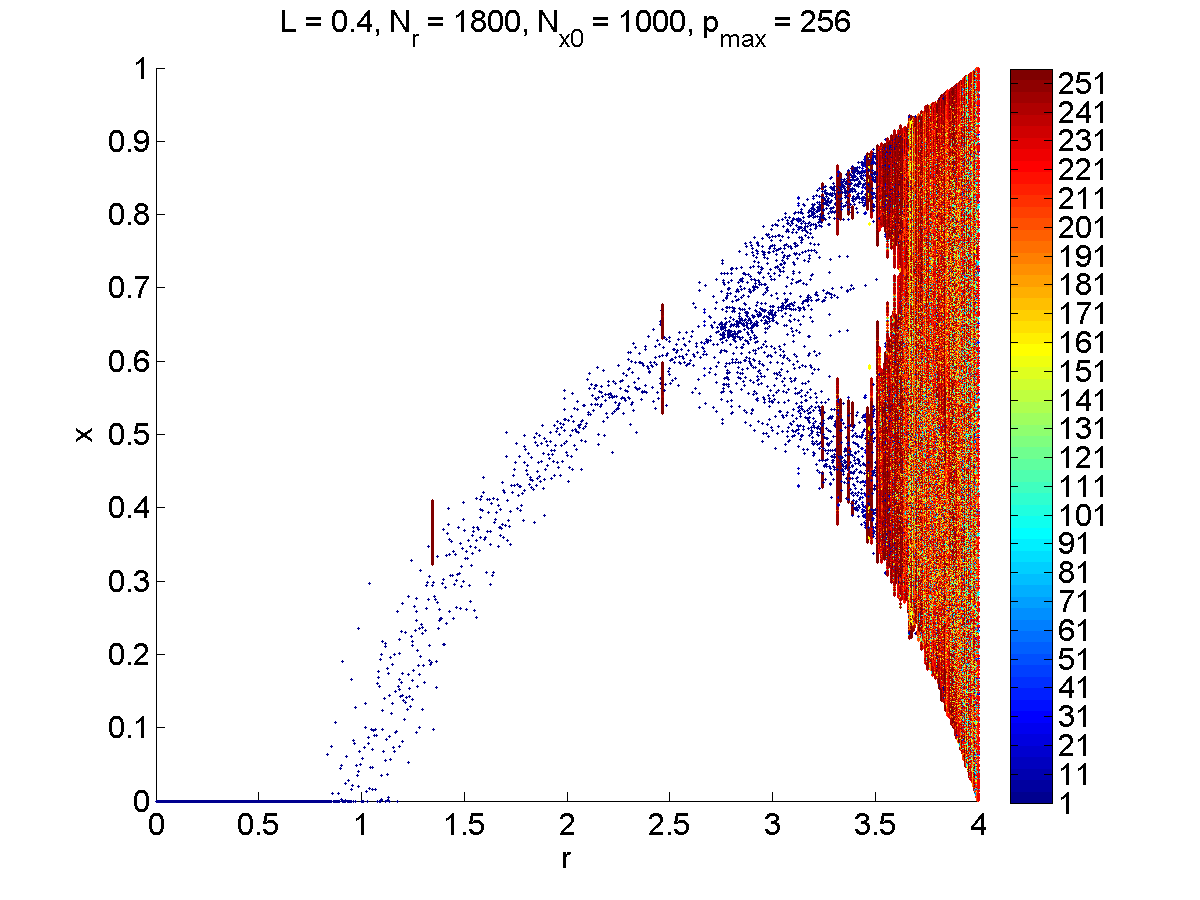
\includegraphics[width=.5\textwidth]{figs/rlog_bif_halfs_L_04.png}\hfill
		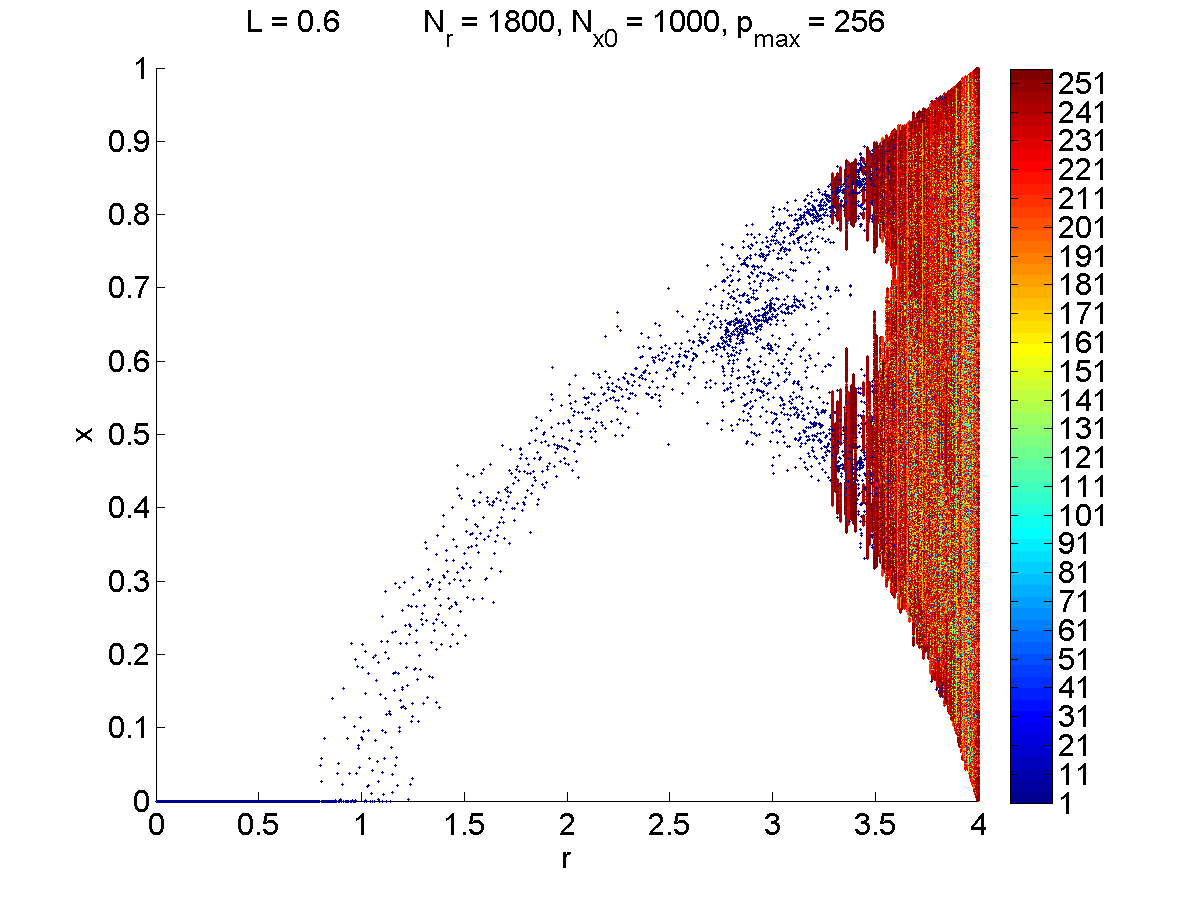
\includegraphics[width=.5\textwidth]{figs/rlog_bif_halfs_L_06.png}\\
		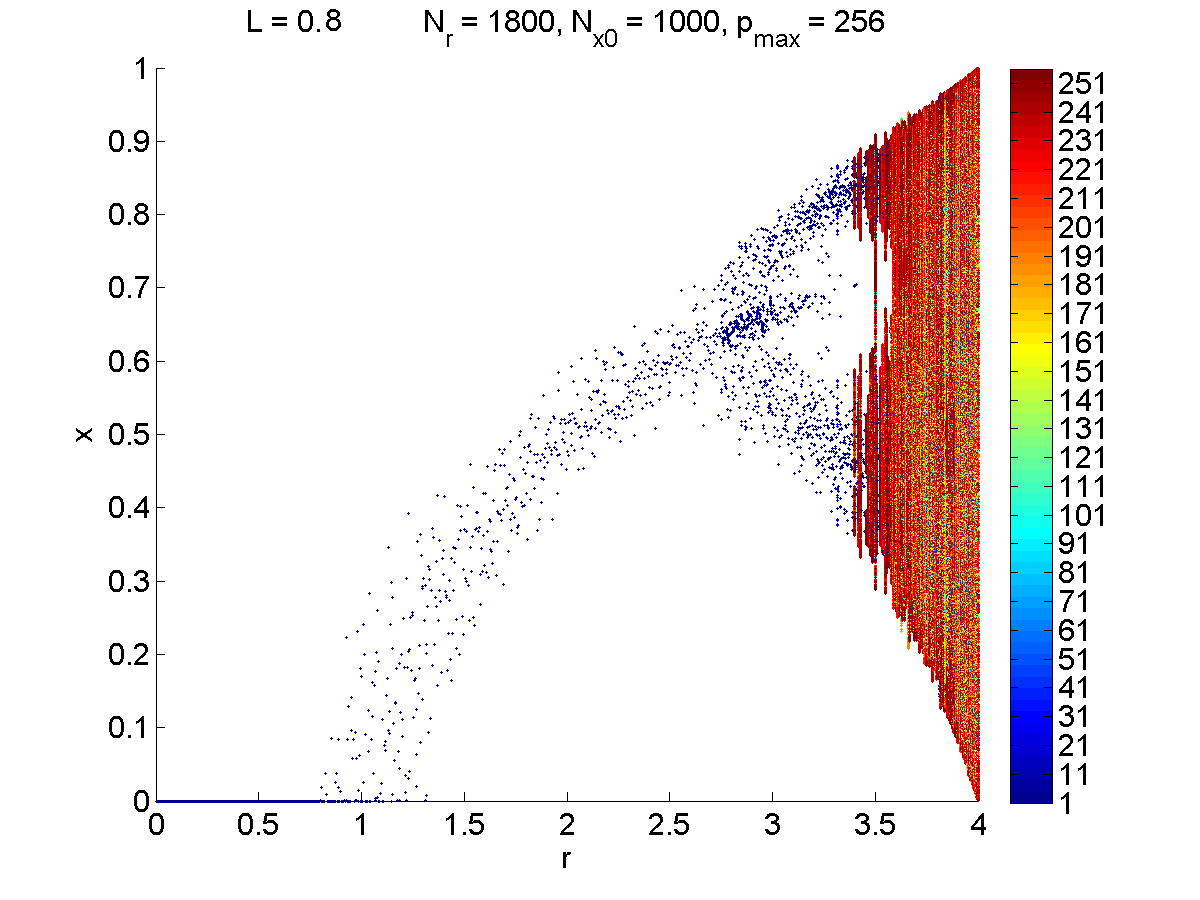
\includegraphics[width=.5\textwidth]{figs/rlog_bif_halfs_L_08.png}\hfill
		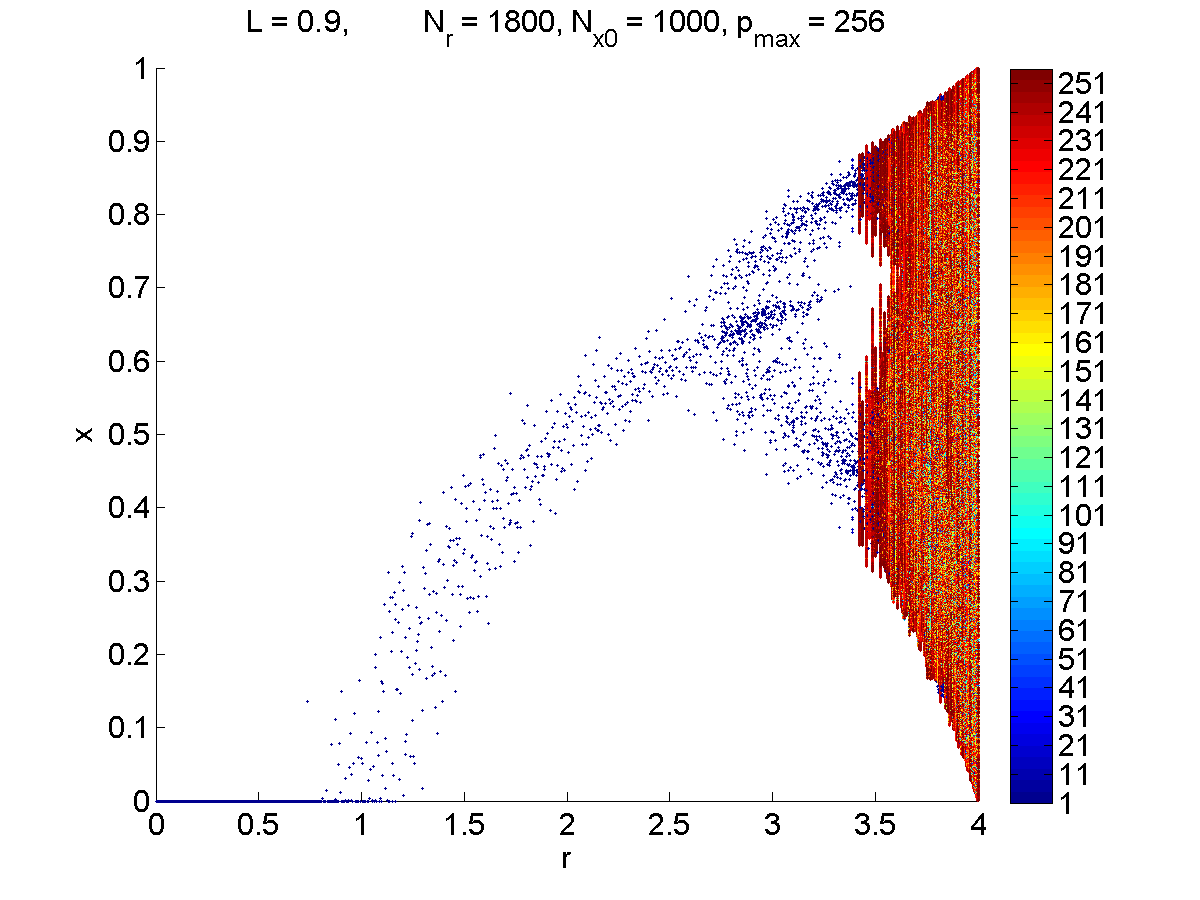
\includegraphics[width=.5\textwidth]{figs/rlog_bif_halfs_L_09.png}\\
	\end{center}
\end{figure}
\begin{figure}[!h]
\caption[Lyapunov exponent in the random logistic map compared to the
deterministic map, $\sigma=\frac{1}{2}\sigma_{max}$]{The Lyapunov exponent for the deterministic
  logistic map (top left) is compared
  to the Lyapunov exponent of the random logistic map for $L \in
  \{0.05,0.1,0.4,0.8,0.9\}$, where $x_0=0.7$ for $r \in [3,4]$, and
  $\sigma$ is chosen to be half of the maximal value in the interval
  from~(\ref{sigma}). The number of exponents computed was $N_\lambda=10,000$. Plots are read left to right, and top to bottom. }\label{fig:rloglyap2_hs}
\centering
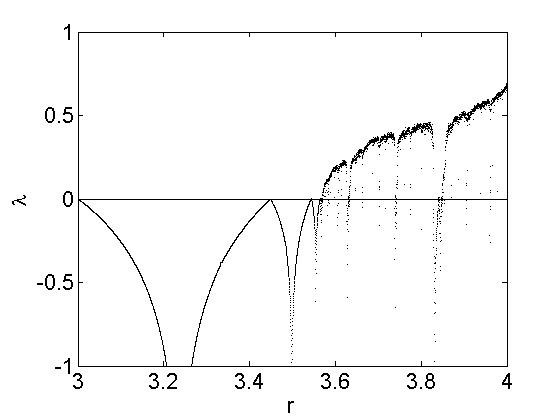
\includegraphics[width=.5\textwidth]{figs/det_log_lyap.png}\hfill
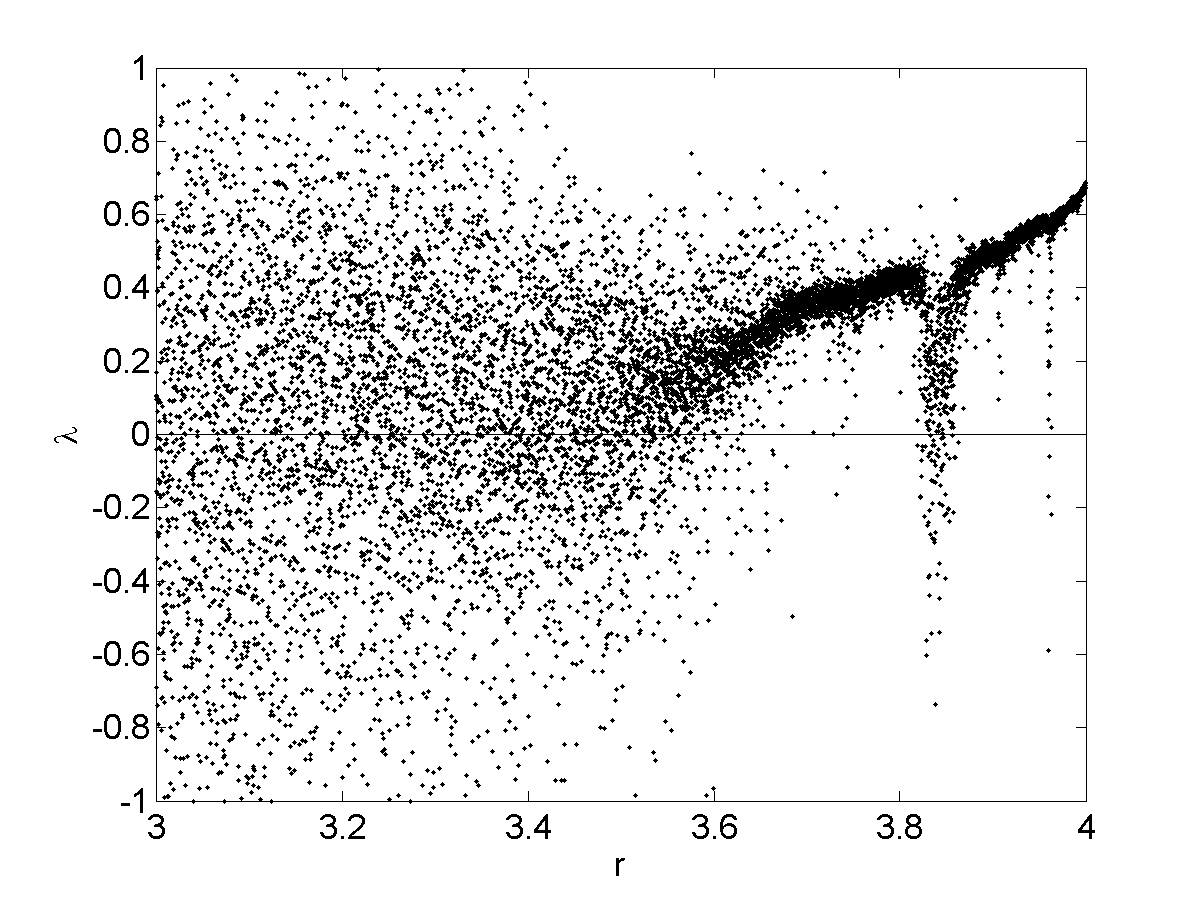
\includegraphics[width=.5\textwidth]{figs/rlog_lyap_halfsig_L_005.png}\\
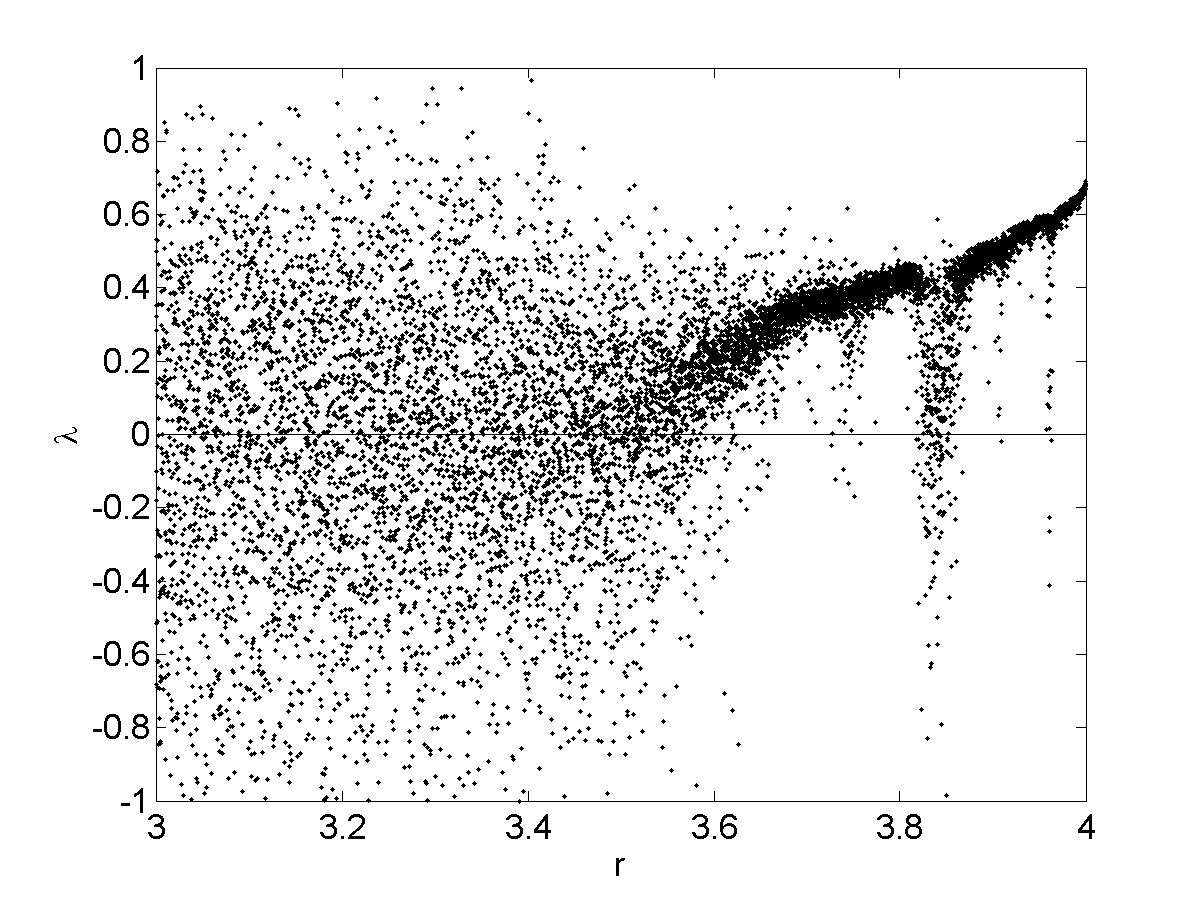
\includegraphics[width=.5\textwidth]{figs/rlog_lyap_halfsig_L_01.png}\hfill
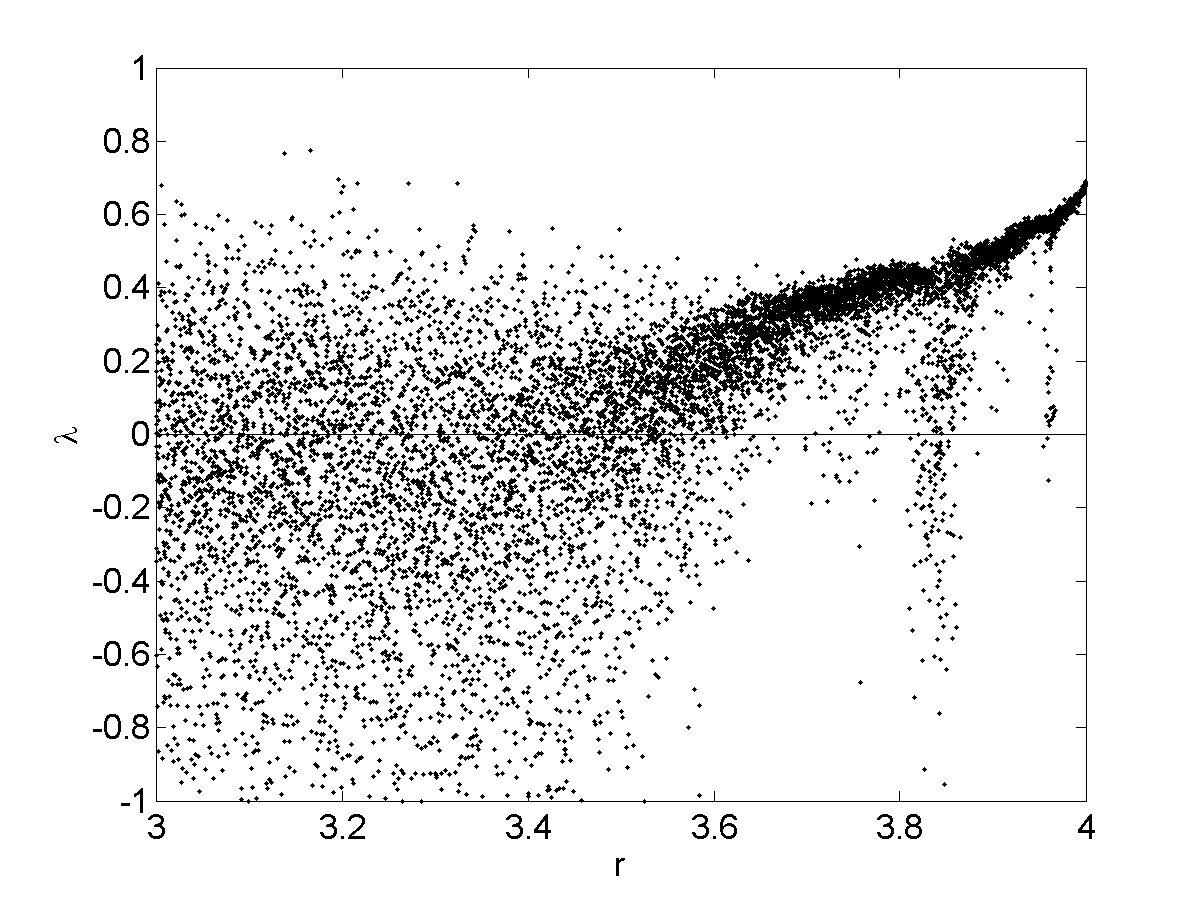
\includegraphics[width=.5\textwidth]{figs/rlog_lyap_halfsig_L_04.png}\\
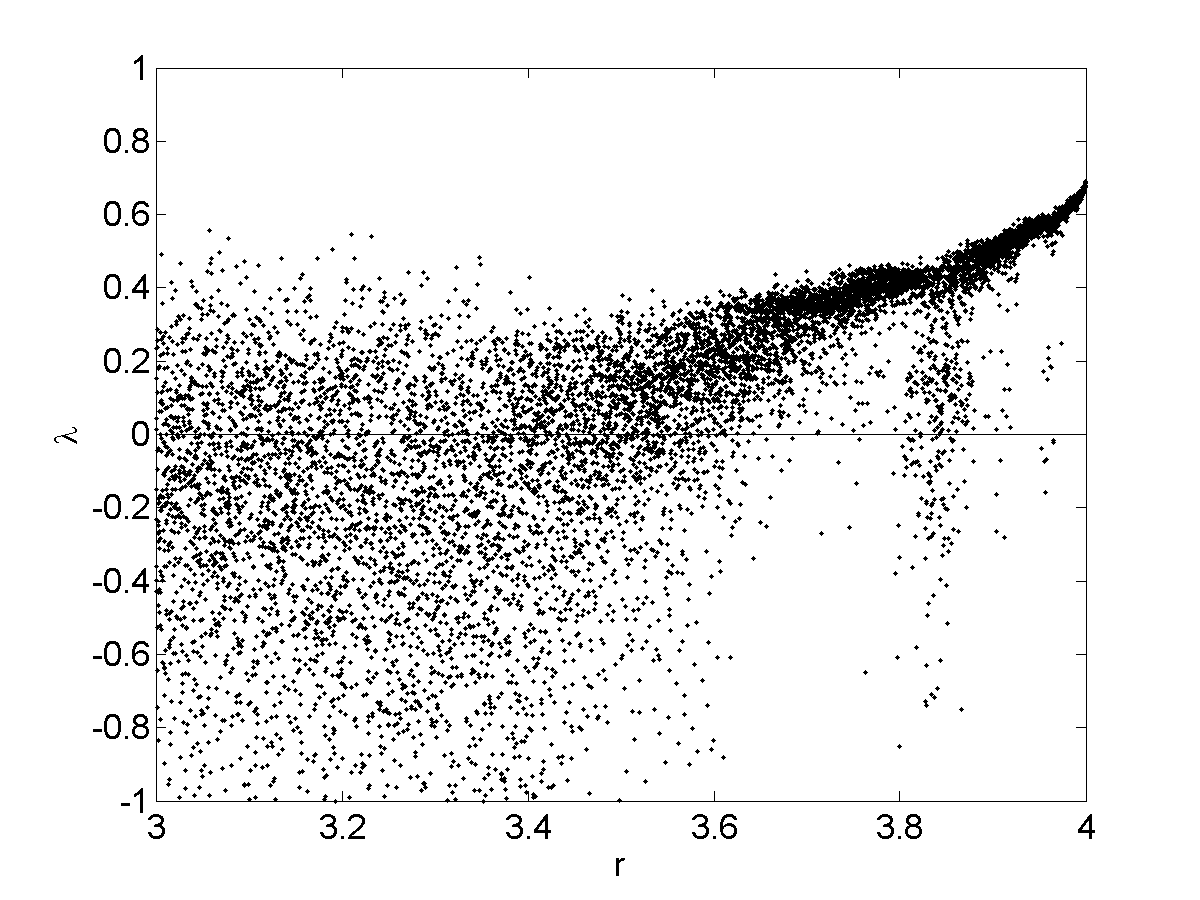
\includegraphics[width=.5\textwidth]{figs/rlog_lyap_halfsig_L_08.png}\hfill
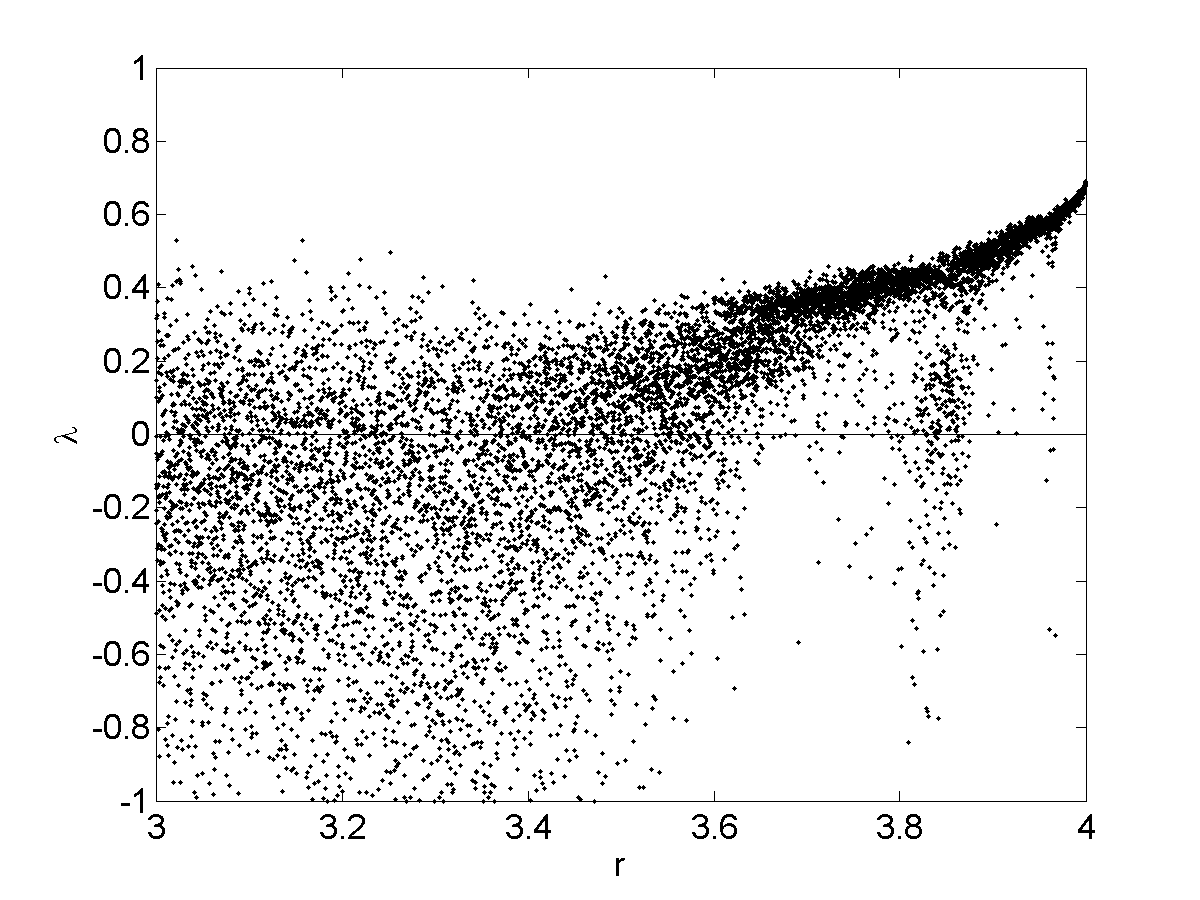
\includegraphics[width=.5\textwidth]{figs/rlog_lyap_halfsig_L_09.png}\\
\end{figure}

For the case where $\sigma = \frac{1}{2}\sigma_{max}$, a histogram describing the average fraction of observed period $p$
orbits is shown in Figure~\ref{fig:rloghist_hs}
and~\ref{fig:rloghist2_hs}. These histograms confirm the observation
that reducing $\sigma$ causes the map to resemble the deterministic
map more closely, which is also shown in Figure~\ref{fig:rlogbif_hs},
the bifurcation diagrams. The frequency of high-period orbits is much
lower in Figure~\ref{fig:rloghist_hs} and~\ref{fig:rloghist2_hs} than
in Figure~\ref{fig:rloghist} and~\ref{fig:rloghist2}, where
$\sigma$ is twice as large. Nonetheless, the general trend in Figure~\ref{fig:rloghist_hs}
and~\ref{fig:rloghist2_hs} implies the distribution of period is
exponential, even for a reduced $\sigma$.

\begin{figure}[H]\linespread{1}
\caption[Average number of period $p$ orbits for the random logistic
map, $\sigma=\frac{1}{2}\sigma_{max}$ and $r=3.22$]{Average number of period $p$ orbits for the random logistic
map, where 5000 simulations are plotted. The error bars indicate
the standard error of the calculation of the mean. In all plots,
$r=3.22$ and $\sigma=\frac{1}{2}\sigma_{max}$. For $(L,N,\sigma)$,
we have $(0.025, 400, 0.0049504)$ (left), $(0.05, 200, 0.0070012)$
(middle), and $(0.1, 100, 0.0099027)$ (right).}\label{fig:rloghist_hs}
	\begin{center}
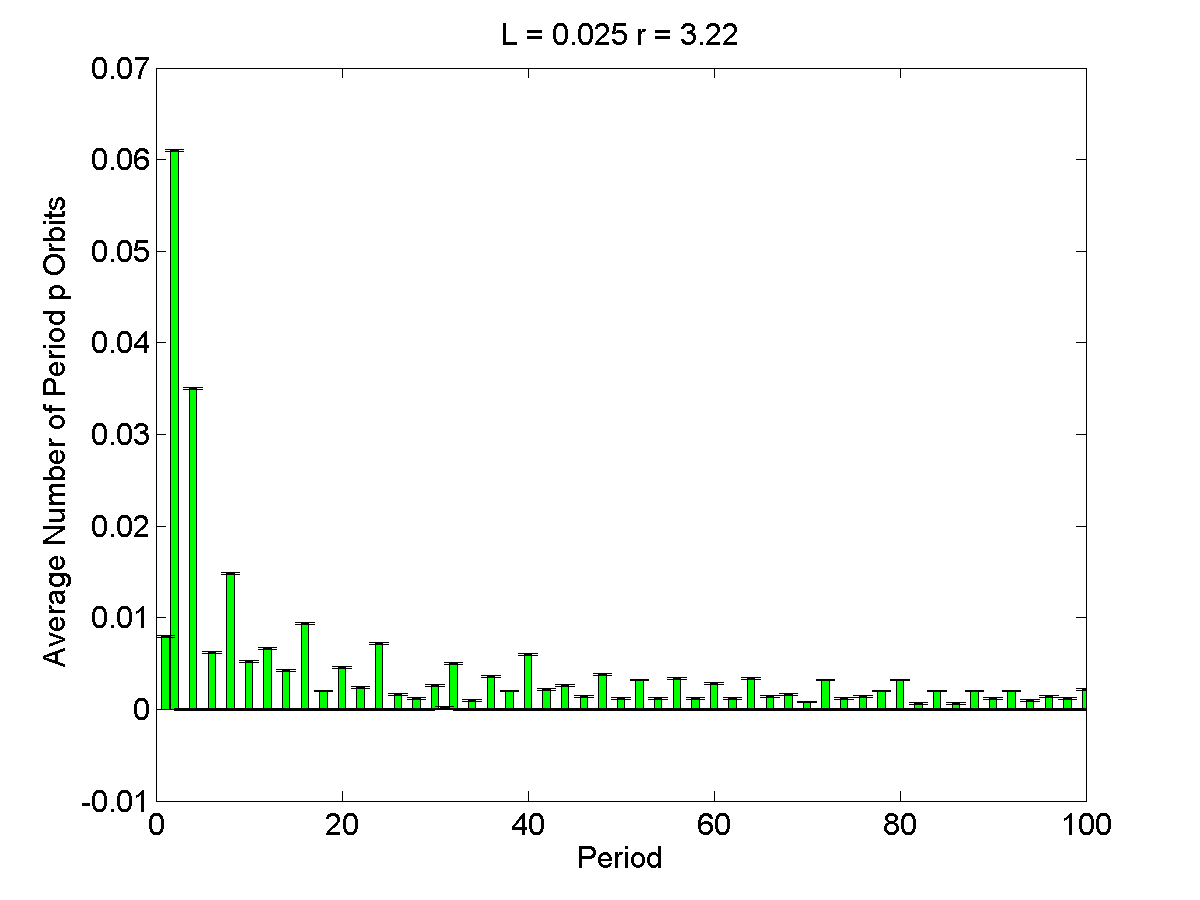
\includegraphics[width=.33\textwidth]{figs/rlog_hist_hs_L_0025_r_322_s_00049504_a_30632e-07_sims_5000.png}\hfill		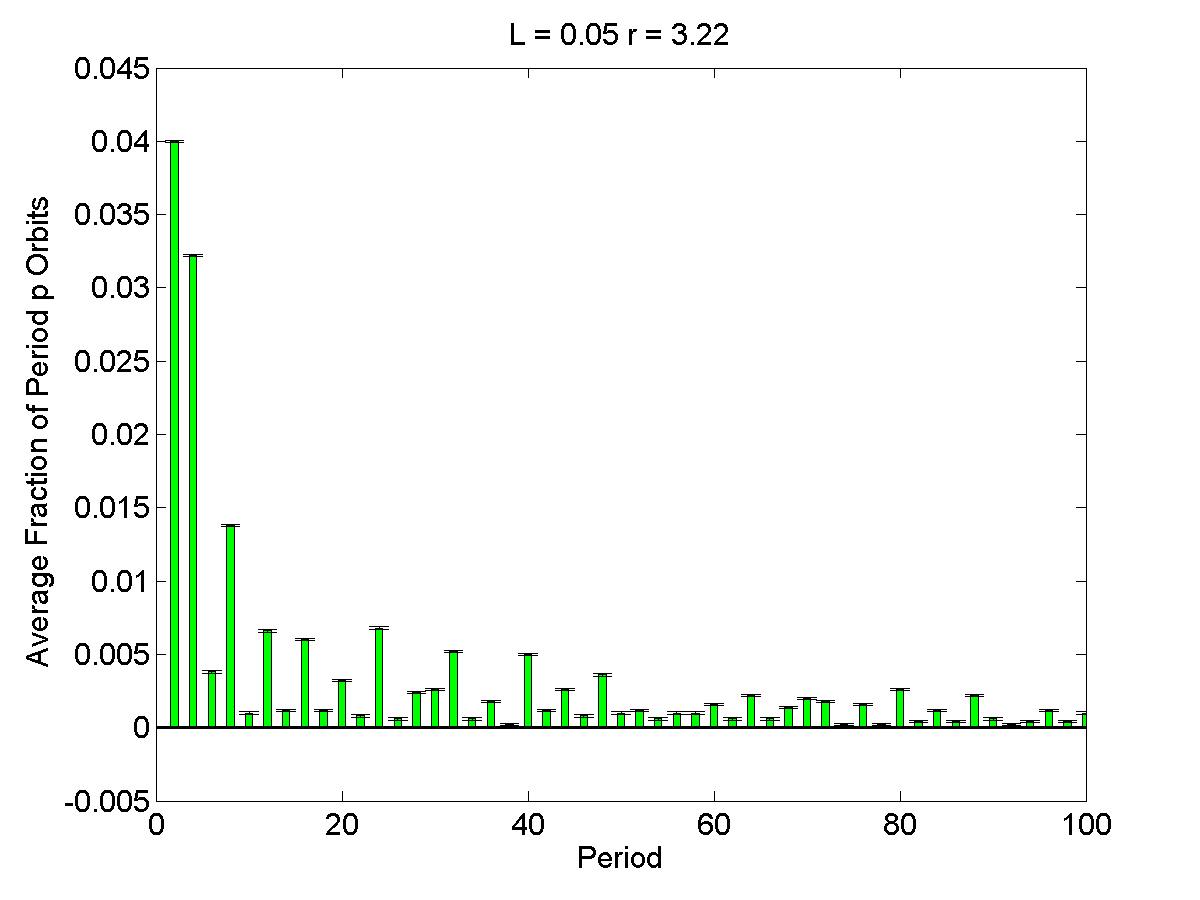
\includegraphics[width=.33\textwidth]{figs/rlog_hist_hs_L_005_r_322_s_00070012_a_12252e-06_sims_5000.png}\hfill
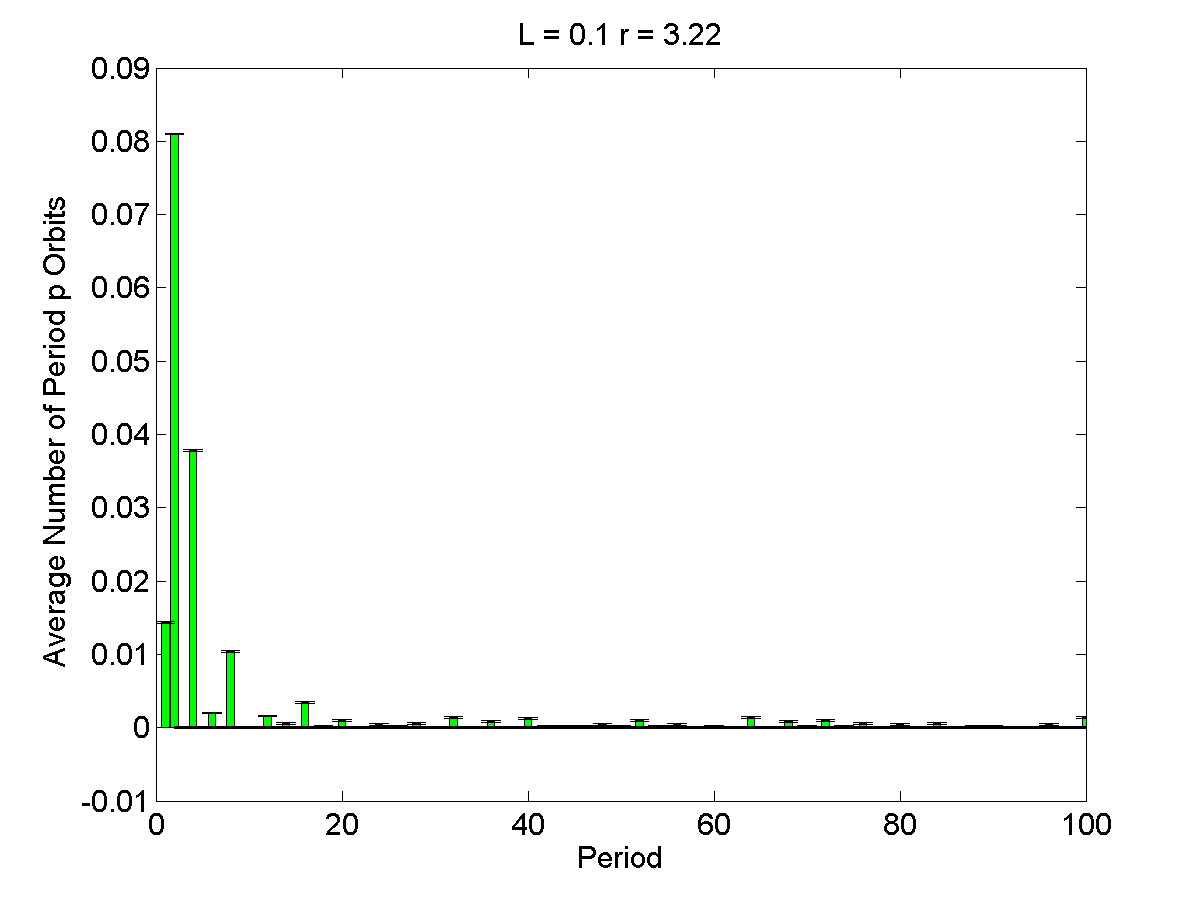
\includegraphics[width=.33\textwidth]{figs/rlog_hist_hs_L_01_r_322_s_00099027_a_48991e-06_sims_5000.png}
	\end{center}
\end{figure}

\begin{figure}[H]\linespread{1}
\caption[Average number of period $p$ orbits for the random logistic
map, $\sigma=\frac{1}{2}\sigma_{max}$ and $r=1.86$]{Average number of period $p$ orbits for the random logistic
map, where 5000 simulations are plotted. The error bars indicate
the standard error of the calculation of the mean. In all plots,
$r=1.86$ and $\sigma=\frac{1}{2}\sigma_{max}$. For $(L,N,\sigma)$,
we have $(0.05, 200, 0.024715)$ (left), $(0.1, 100, 0.034957)$
(middle), and $(0.3, 100, 0.060648)$ (right).}\label{fig:rloghist2_hs}
	\begin{center}	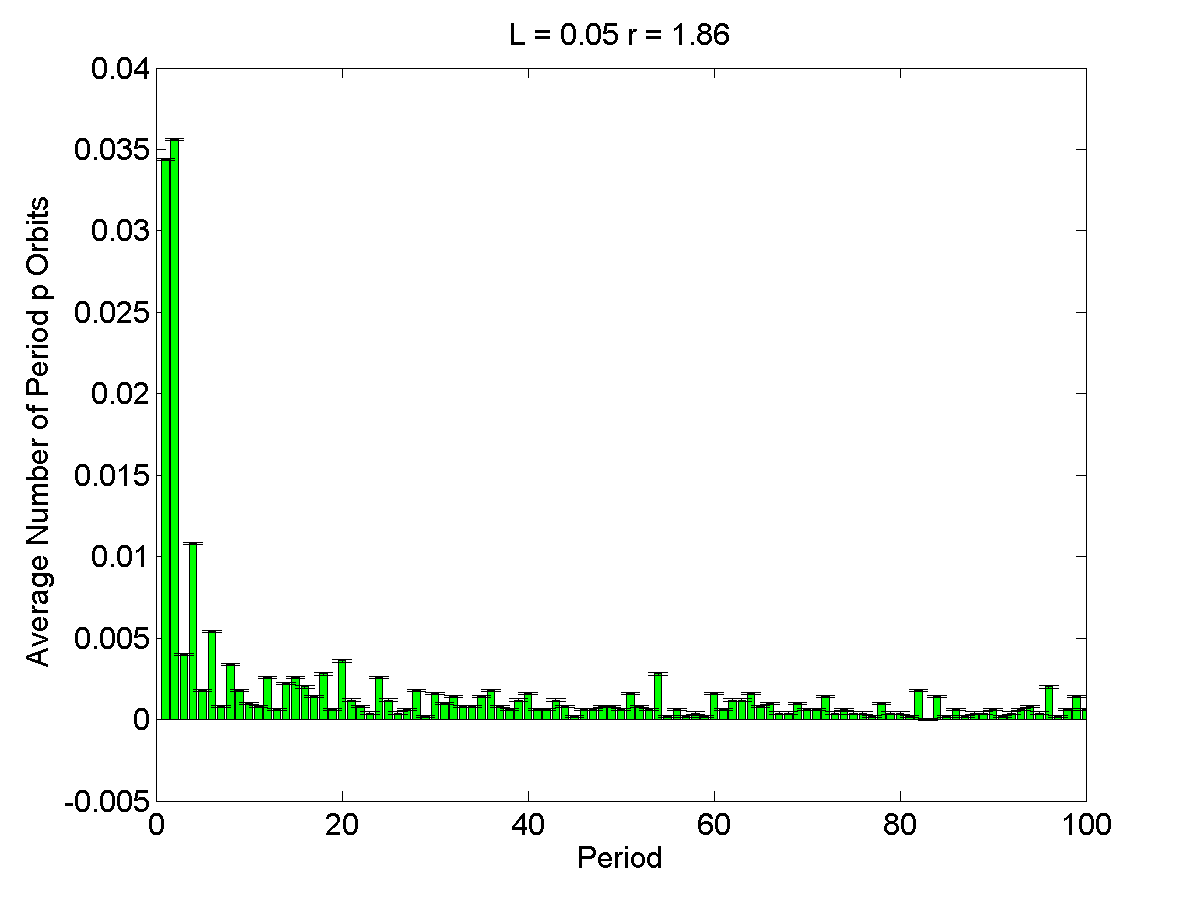
\includegraphics[width=.33\textwidth]{figs/rlog_hist_hs_L_005_r_186_s_0024715_a_15267e-05_sims_5000.png}\hfill
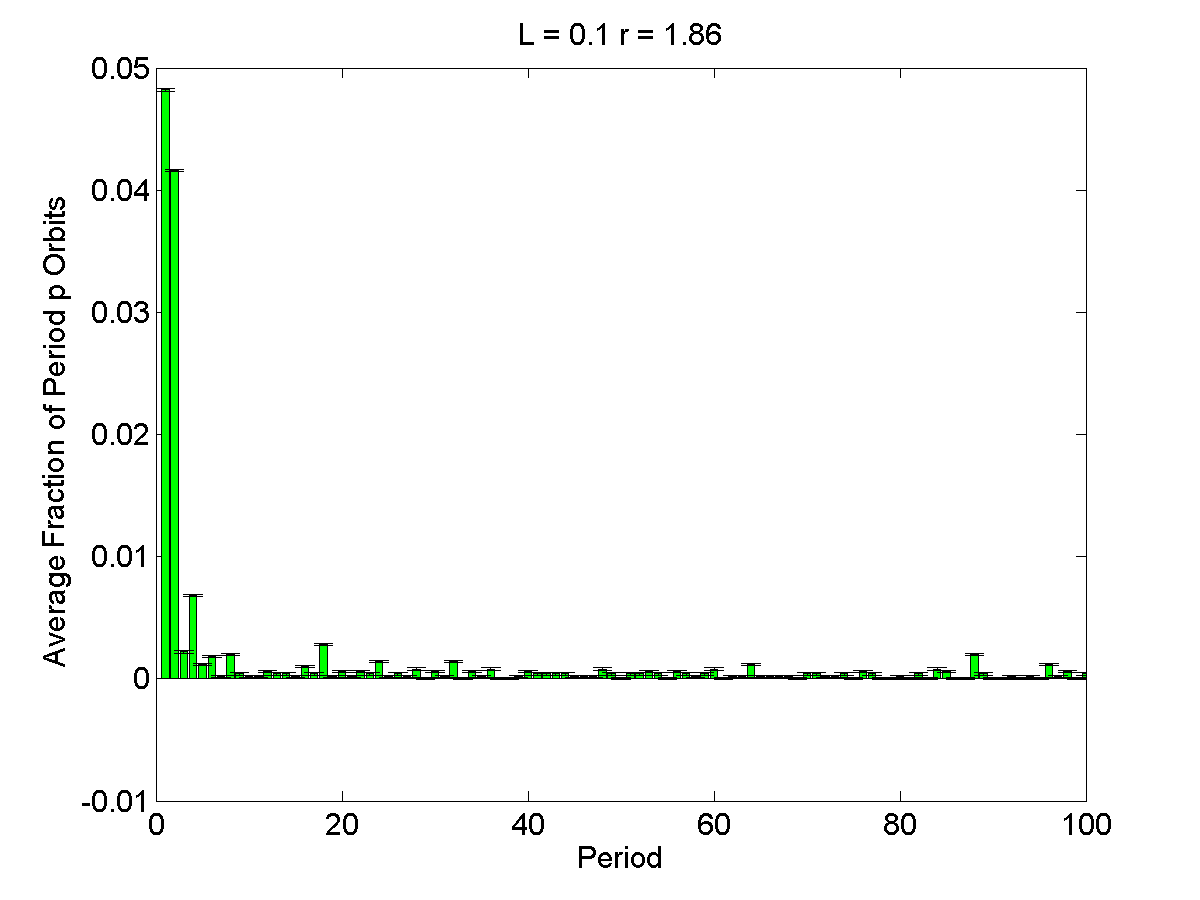
\includegraphics[width=.33\textwidth]{figs/rlog_hist_hs_L_01_r_186_s_0034957_a_6105e-05_sims_5000.png}\hfill	
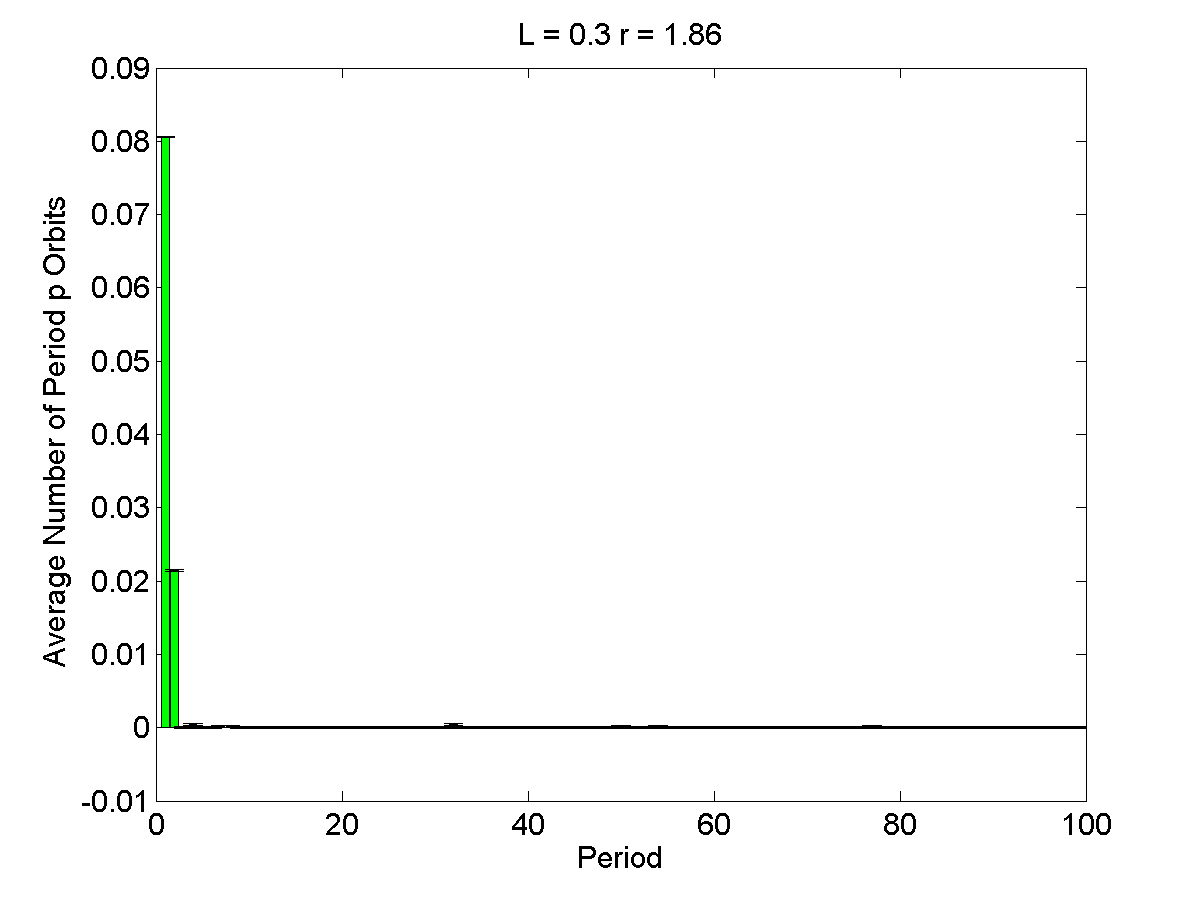
\includegraphics[width=.33\textwidth]{figs/rlog_hist_hs_L_03_r_186_s_0060648_a_000054762_sims_5000.png}
	\end{center}
\end{figure}

\section{Implementation of Randomness in the Circle Map}
We explored how the random circle map for uniformly distributed $\hat{\xi}_n$ and
normally distributed $\hat{\xi}_n$ changes in terms of its Arnold
tongues, devil's staircases, Lyapunov exponents, and periodic orbit distribution. We examined the
distribution of rotation numbers using a kernel density
estimator. Histograms of the observed frequency of a period $p$ orbit
attempt to describe the period distribution in the random circle
map. The parameter $\alpha$ that scales the variance of the Fourier
modes of the spatial process $\xi(x)$ from~(\ref{spec}) was tested for two values: $\alpha=10^{-5}$
and $\alpha = \frac{1}{2}10^{-5}$. This parameter also scales the
covariance of $\xi(x)$. These two values were explored in
the case where $\hat{\xi}_n$ was uniformly and normally distributed.

In the Arnold tongue diagrams 
(Figure~\ref{fig:rcirctongues_u},~\ref{fig:rcirctongues_u_ha},~\ref{fig:rcirctongues_n},~\ref{fig:rcirctongues_n_ha}), each value of $k \in
[0,1.5]$ and $\omega \in [0,1]$ was tested according to the
discretization of $\Delta k=0.0015, \Delta \omega = 0.001$ and initial
condition $x_0=0.7$. If iterating the map for any given set of
parameters resulted in finding no periodic orbit of period $p_{max}$
or less, then the pixel corresponding to this value of $(\omega, k)$
was colored black. Otherwise, the pixel for this $(\omega, k)$ pair was colored
according to the orbit period. An orbit was
denoted period $p$ if, after iterating the map 1,000 times,
$x_p=x_{n+p}$ within a tolerance of $\epsilon = 10^{-6}$.

Plotting the change in rotation number $\rho$ as $\omega$ is varied over
$[0,1]$ results in a devil's staircase. The figures relating to the
devil's staircase fixed a value of $L$ and $k$ over 10,000 values of
$\omega \in [0,1]$. Each $L$ tested had the same set of Fourier
modes $\hat{\xi}_n$ for all 10,000 $\omega$ values. The lift of the circle map was used to find the
rotation number, and it was assumed that iterating the lift 1,000
times was enough to converge on a rotation number, if one exists. 

The Lyapunov exponents for the random map were calculated according to
the formula in~(\ref{eq:lyap}) with $N_\lambda=n=10,000$. For the circle map, 
\begin{align}
\begin{split}
\lambda(x_0) &= \frac{1}{n} \sum_{i=0}^{n-1} \ln |f'(x_i)|\\
&= \frac{1}{10000} \sum_{i=0}^{9999} \ln |1 + \Omega'(x_i) - k\cos(2\pi x_i)|\\
&= \frac{1}{10000} \sum_{i=0}^{9999} \ln |1+e^{\xi(x_i)}\xi'(x_i)- k\cos(2\pi x_i)|.
\end{split}
\end{align}
Values of $\omega$ were chosen in $[0,1]$ with stepsize $\Delta \omega
= 0.001$ for the case where $k$ was fixed, and values of $k$ were
chosen in $[0,5]$ with stepsize $\Delta k = 0.005$ for the case where
$\omega$ was fixed. The initial condition $x_0$ was fixed for all
simulations at $x_0=0.7$.

To produce the histograms, 10 random initial conditions $x_0$ were tested 500 times
each, resulting in 5,000 total simulations. Each time any given $x_0$
was tested, a new set of random Fourier modes $\hat{\xi}_n$ were drawn
from either a uniform or normal distribution. After iterating the random
map 1,000 for some $\omega,k$ pair and this set of random variables, an orbit was denoted period $p$ if $x_p = x_{n+p}$ within a
tolerance of $\epsilon = 10^{-6}$. Periodicity was checked up to
$p_{max}=100$. The histograms count unique periodic orbits, so if two
or more initial conditions converged to the same periodic orbit, only
one was counted. 
\subsection{Uniform Distribution}
The randomized circle map for uniformly distributed $\hat{\xi}_n$ has
a set of Arnold tongues (Figure~\ref{fig:rcirctongues_u} and~\ref{fig:rcirctongues_u_ha}) that has almost no similarity to the deterministic
case. For low values of $L$, we have lost the
shape of the tongues, and the diagram becomes asymmetrical. For larger
values of $L$, the distinctive tongues and the overall symmetry is
recovered. The randomness appears to have an overall destabilizing
effect on the dynamics of the map. For $L=0.05$, we also observe the
presence of high-period orbits in the region where there is typically
only period 1 fixed points (upper left). As $L$ increases, this region
morphs into predominantly stable period 1 orbits. 

For $L=0.05$, there is a noticeable lack of high-period orbits for
$\omega<0.2$ when $\alpha = \frac{1}{2}10^{-5}$
(Figure~\ref{fig:rcirctongues_u_ha}) compared to the case where
$\alpha = 10^{-5}$ (Figure~\ref{fig:rcirctongues_u}). In addition to
this observation, when $L=0.3$, there is a region of stable period 2
orbits for $\omega > 0.9$ when $\alpha = \frac{1}{2}10^{-5}$, yet this
region is absent for $\alpha = 10^{-5}$. Also, the stable period 4
region for $\omega \approx 0.5$ is much smaller when $\alpha$ is half
as large. Increasing $\alpha$ seems to increase the number of
high-period orbits for certain values of $\omega < 0.2$, eliminate period
2 orbits when $\omega >0.9$, and reduce the number of period 4 orbits
in the center tongue. 

Figure~\ref{fig:rcirclyap_u} is a plot of the Lyapunov
exponents for a fixed $k$ and varying $\omega$, whereas
Figure~\ref{fig:rcirclyap2_u} fixes $\omega$ and varies $k$. A comparison of the Lyapunov exponent of the deterministic and random
case (Figure~\ref{fig:rcirclyap_u} and Figure~\ref{fig:rcirclyap2_u})
partially confirms the idea that the noise is destabilizing; nearly no
features of the deterministic graph are preserved (for small $L$), and the high
density of positive values indicates chaotic
behavior. Moreover, Figure~\ref{fig:rcirclyap_u} demonstrates that there is a skewed
distribution of Lyapunov exponents on the right side of the graph for
all values of $L$, compared to the left side. However, this trend is
not observed in Figure~\ref{fig:rcirclyap2_u}.

% In Figure~\ref{fig:rcirc_bifw_u}, it appears that as $\omega$ is
% varied over $[0,1]$ (for fixed $k=1$), the distribution of stable
% orbits follows the line $x=\omega$. However, closer examination of the
% solutions of (\ref{randcirc}) demonstrate
% \begin{align*}
% \begin{split}
% \omega &= \frac{k}{2\pi}\sin(2\pi x)\\
% x &= \frac{1}{2\pi}\arcsin\left(\frac{2\pi \omega}{k}\right).
% \end{split}
% \end{align*}

\begin{figure}[H]\linespread{1}  
\caption[The Arnold tongues for the random circle map, uniform
distribution, $\alpha = 10^{-5}$]{The Arnold
  tongues for $k\in [0,1.5]$, $\Delta k = 0.0015$, $\omega \in [0,1]$,
  $\Delta \omega = 0.001$, $\alpha = 10^{-5}$, $\hat{\xi}_n\sim Unif(-M_n,M_n)$ and $L_j \in
  \{0.05,0.1,0.3,0.5,0.7,0.9\}$. $\Delta k$ and $\Delta \omega$
  represent the step size in discretizing $k$ on [0,1.5] and $\omega$
  on [0,1]. Plots are ordered left to right,
  and top to bottom. The colorbar to the right demonstrates the period and corresponding color.}\label{fig:rcirctongues_u}
\centering
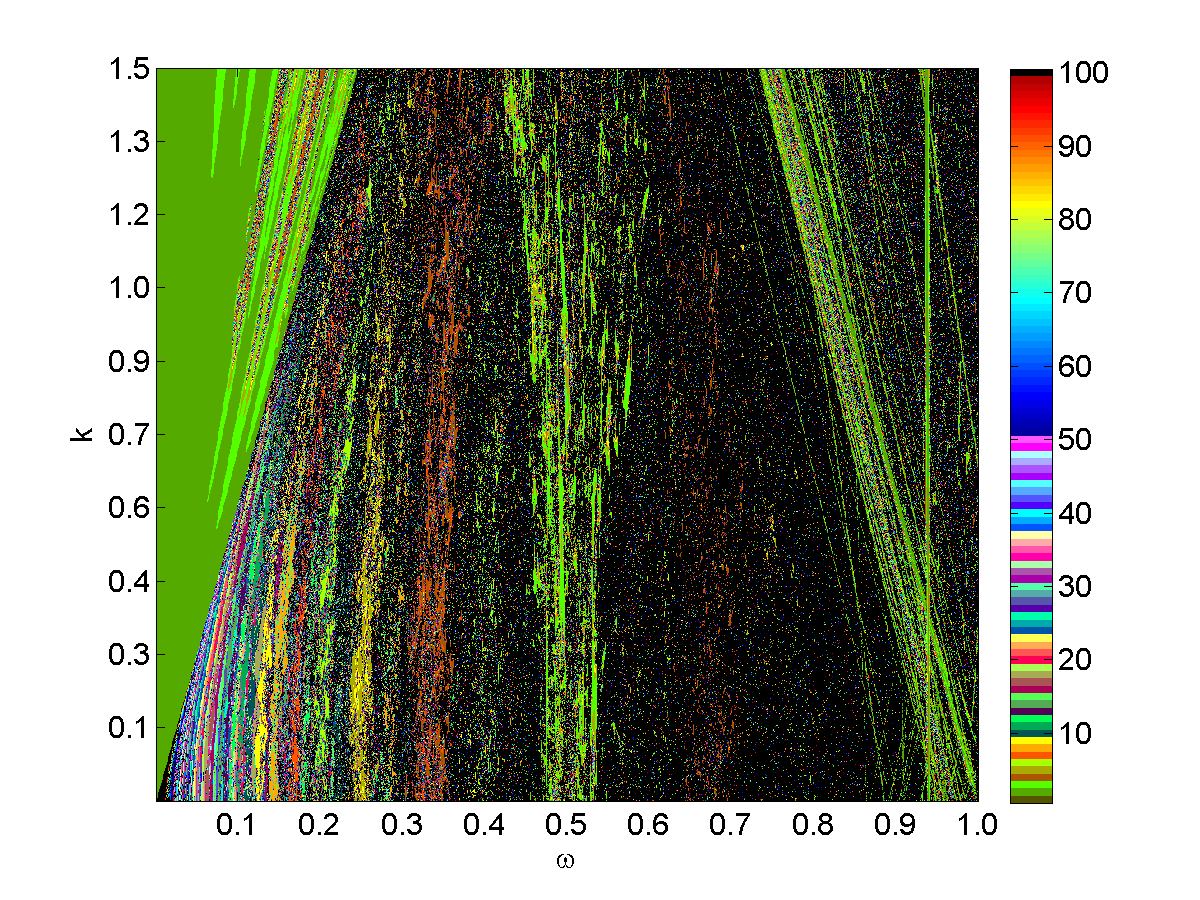
\includegraphics[width=.5\textwidth]{figs/tongues_1000_L_005.png}\hfill
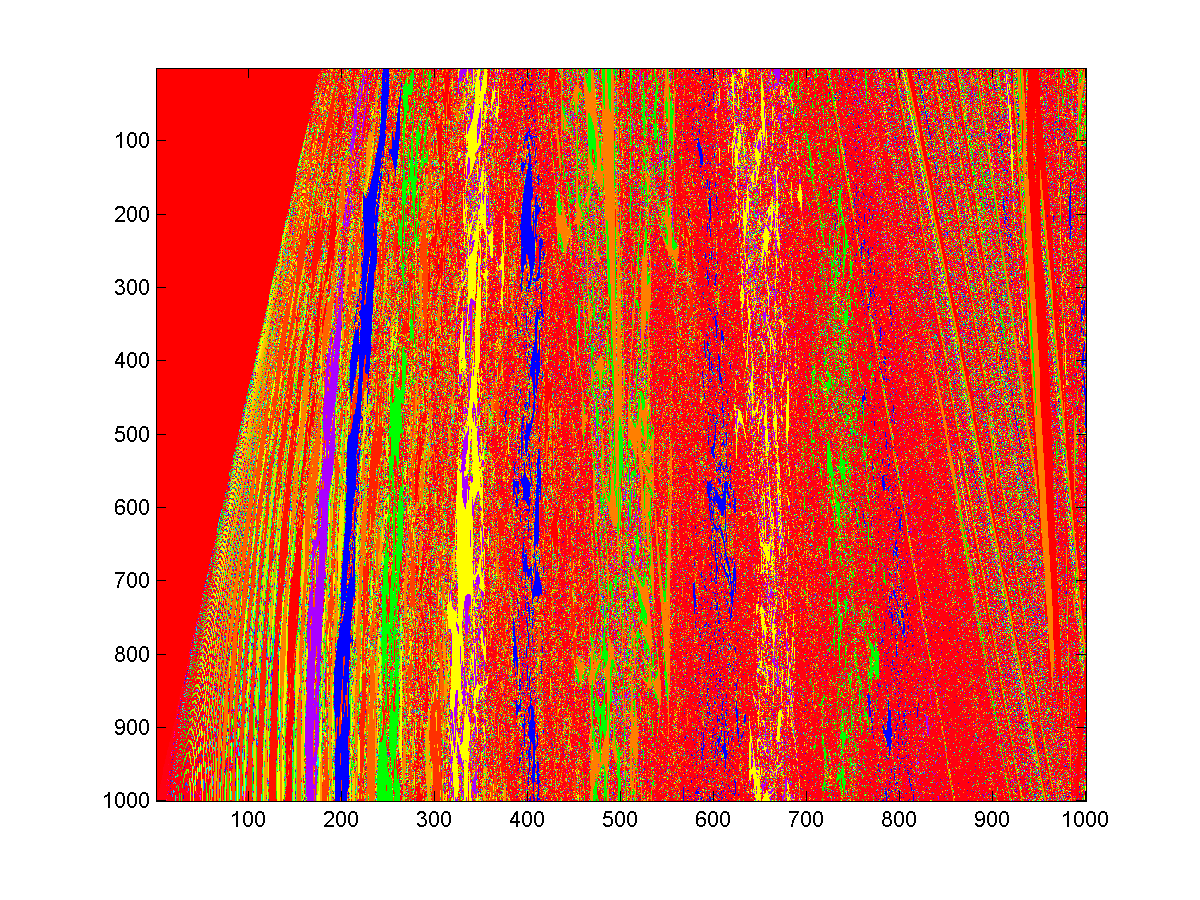
\includegraphics[width=.5\textwidth]{figs/tongues_1000_L_01.png}\\
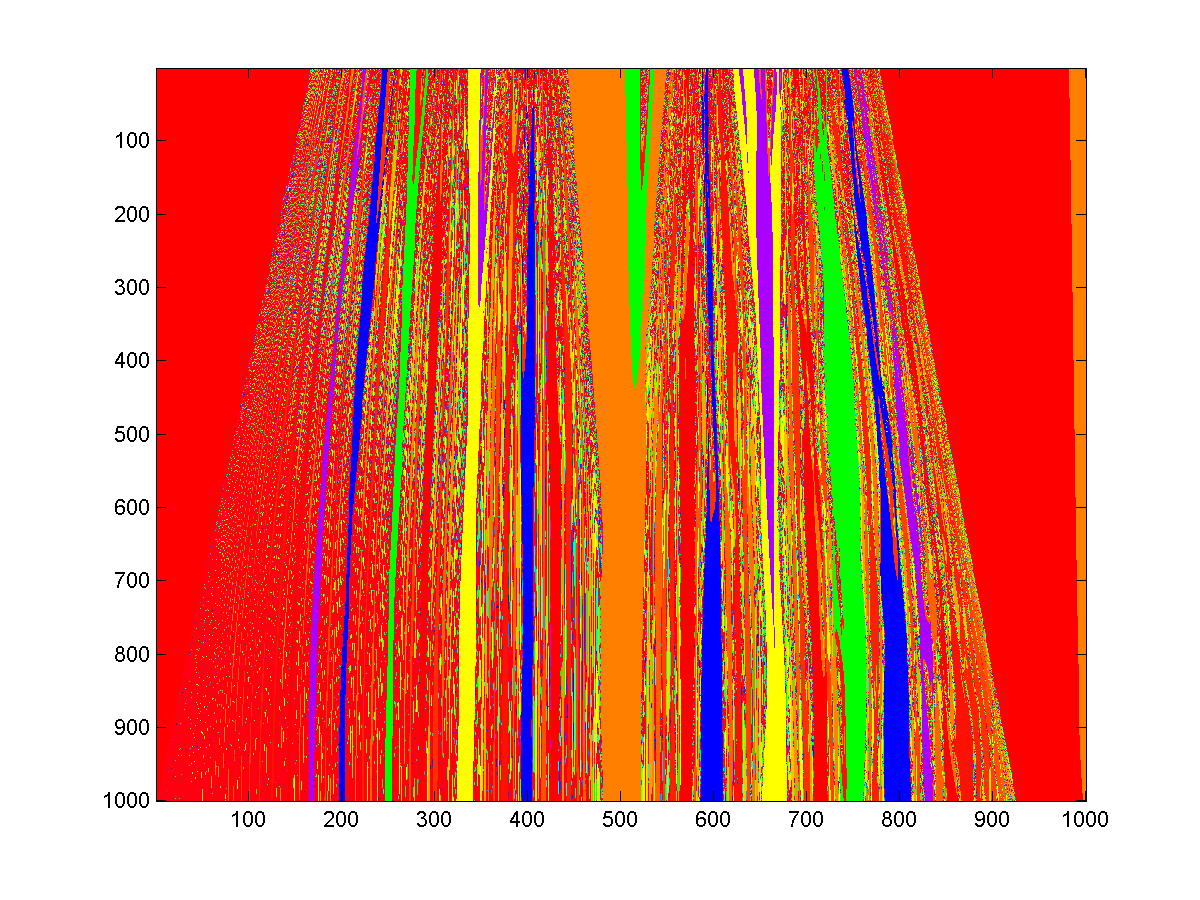
\includegraphics[width=.5\textwidth]{figs/tongues_1000_L_03.png}\hfill
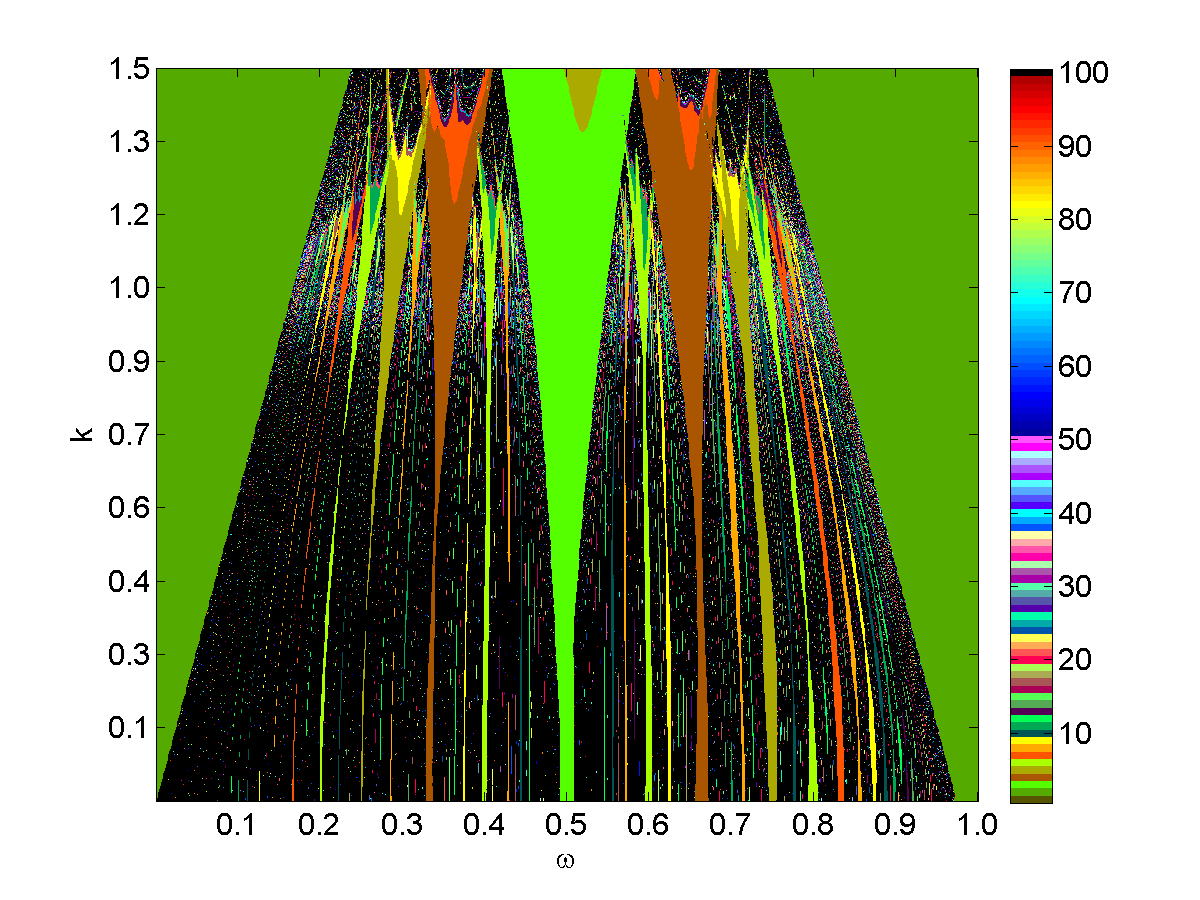
\includegraphics[width=.5\textwidth]{figs/tongues_1000_L_05.png}\\
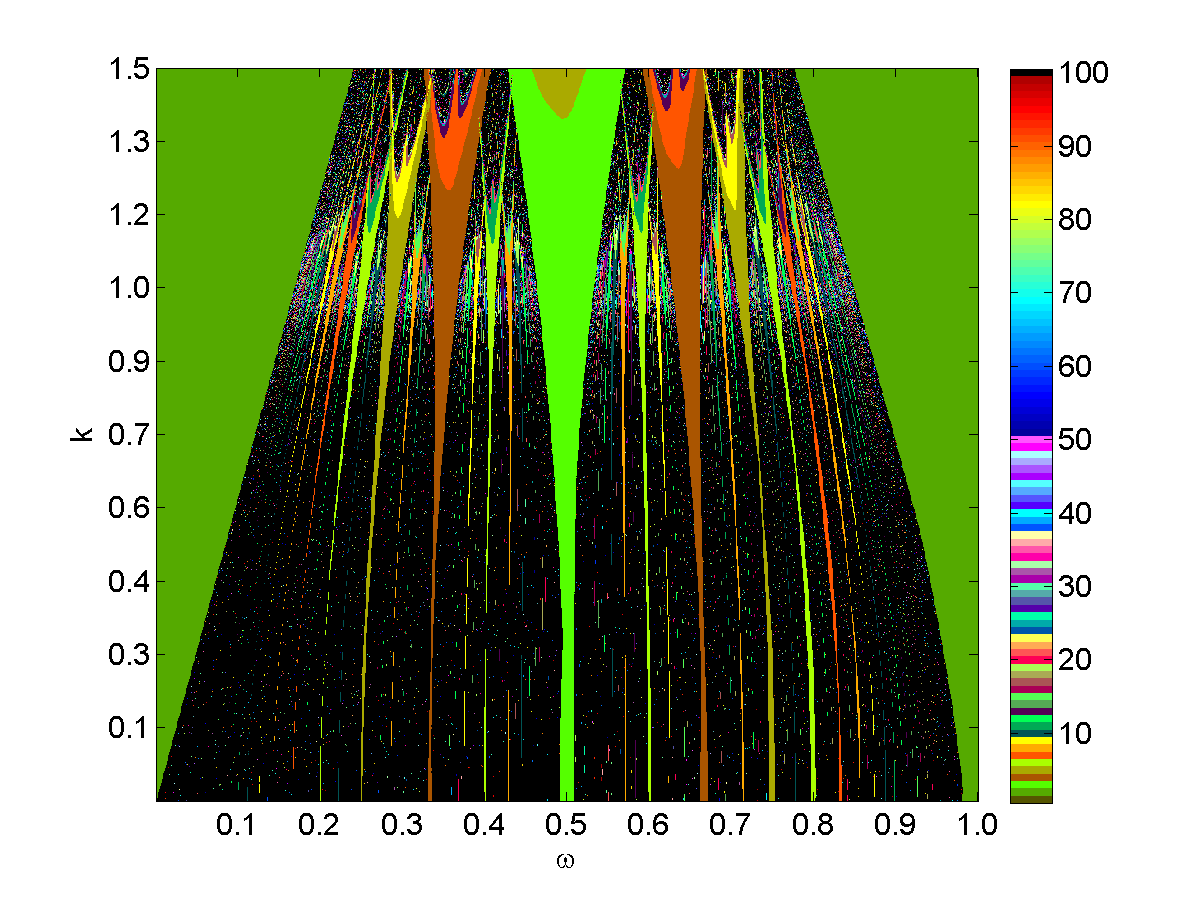
\includegraphics[width=.5\textwidth]{figs/tongues_1000_L_07.png}\hfill
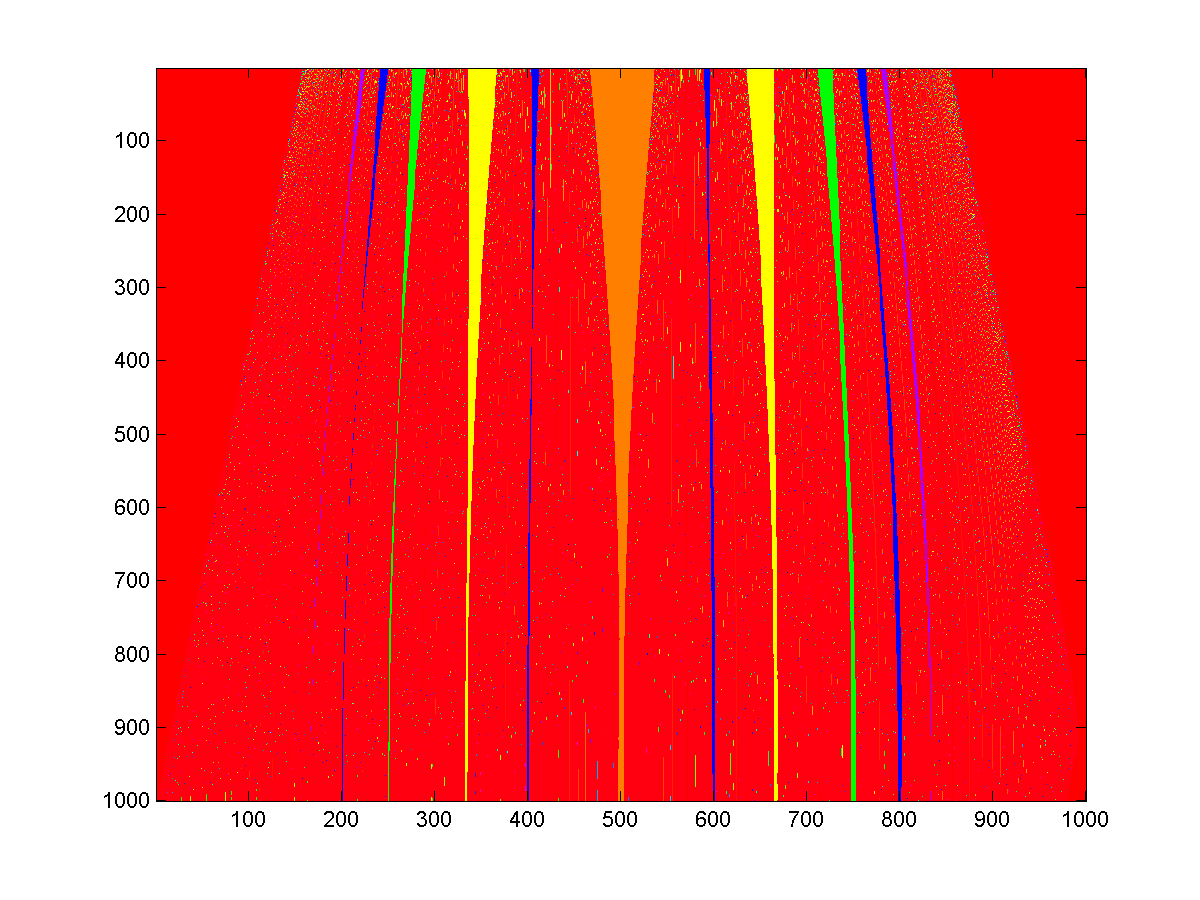
\includegraphics[width=.5\textwidth]{figs/tongues_1000_L_09.png}\\
\end{figure}

\begin{figure}[H]\linespread{1}  
\caption[The Arnold tongues for the random circle map, uniform
distribution, $\alpha = \frac{1}{2}10^{-5}$]{The Arnold
  tongues for $k\in [0,1.5]$, $\Delta k = 0.0015$, $\omega \in [0,1]$,
  $\Delta \omega = 0.001$, $\alpha = 10^{-5}$, $\hat{\xi}_n\sim Unif(-M_n,M_n)$ and $L_j \in
  \{0.025,0.05,0.1,0.3,0.5,0.9\}$. $\Delta k$ and $\Delta \omega$
  represent the step size in discretizing $k$ on [0,1.5] and $\omega$
  on [0,1]. Plots are ordered left to right,
  and top to bottom. The colorbar to the right demonstrates the period and corresponding color.}\label{fig:rcirctongues_u_ha}
\centering
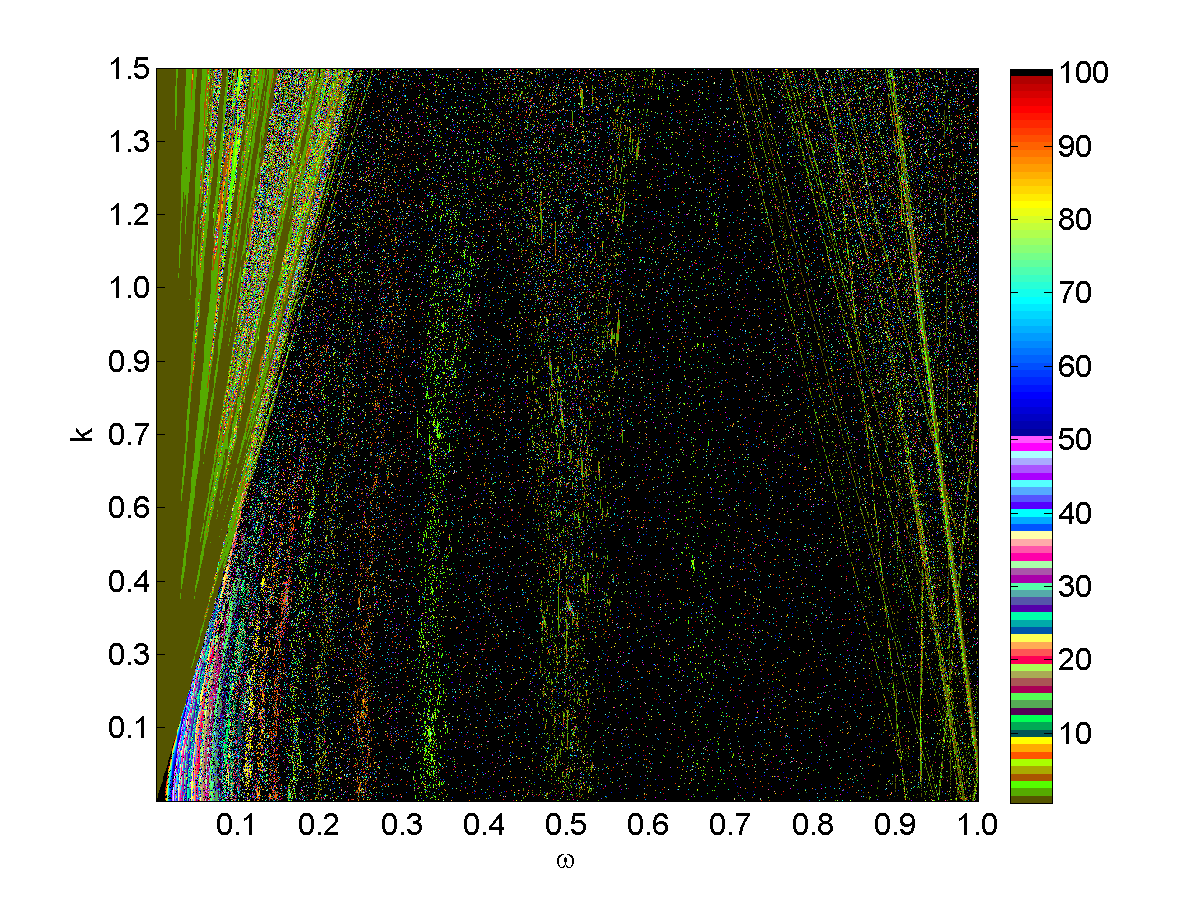
\includegraphics[width=.5\textwidth]{figs/tongues_u_halfa_1000_L_0025.png}\hfill
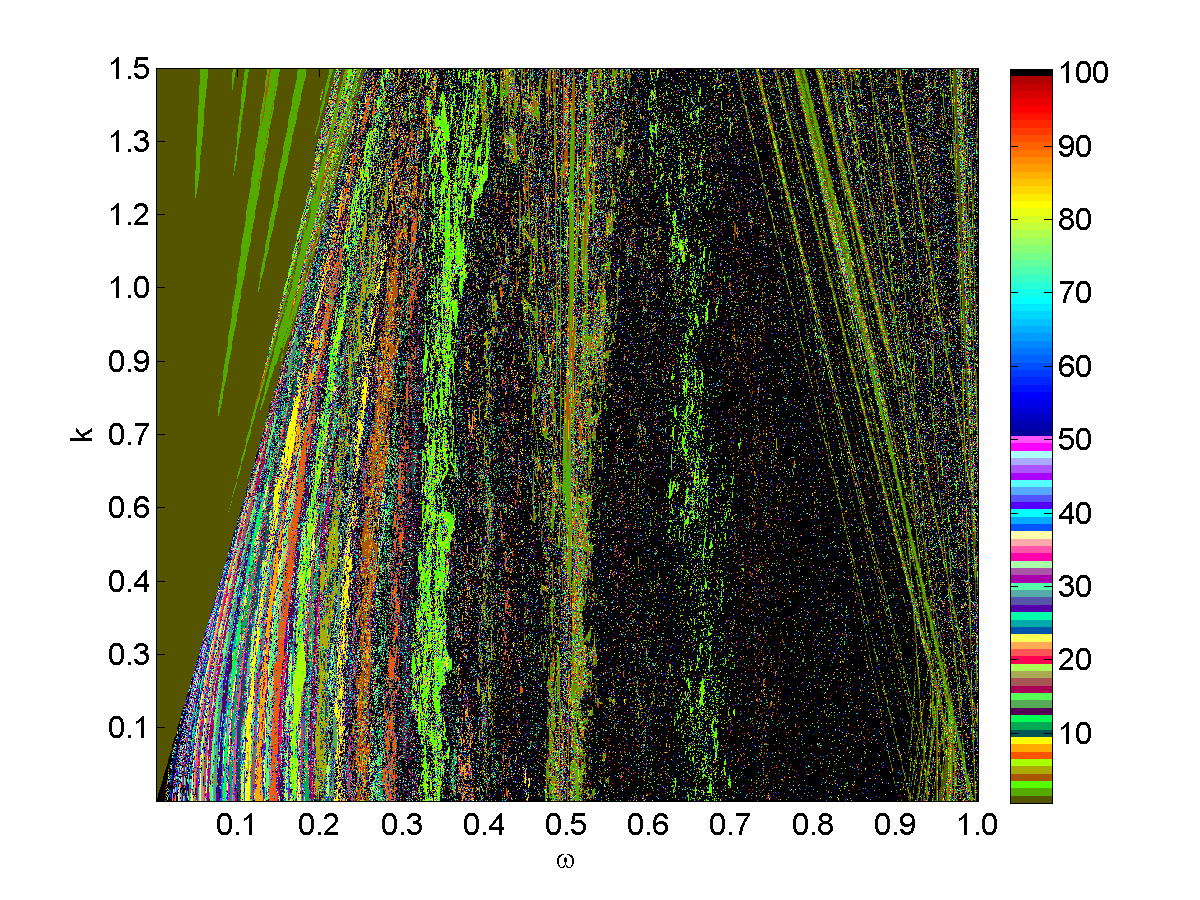
\includegraphics[width=.5\textwidth]{figs/tongues_u_halfa_1000_L_005.png}\\
\includegraphics[width=.5\textwidth]{figs/tongues_u_halfa_1000_L_01.png}\hfill
\includegraphics[width=.5\textwidth]{figs/tongues_u_halfa_1000_L_03.png}\\
\includegraphics[width=.5\textwidth]{figs/tongues_u_halfa_1000_L_05.png}\hfill
\includegraphics[width=.5\textwidth]{figs/tongues_u_halfa_1000_L_09.png}\\
\end{figure}

\begin{figure}[!h]
\caption[Lyapunov exponent in the random circle map (uniform distribution) compared to the
deterministic map, varying $\omega$, $\alpha = 10^{-5}$]{The Lyapunov exponent for the deterministic
  circle map (top left) is compared
  to the Lyapunov exponent of the random circle map for $L \in
  \{0.05,0.1,0.3,0.5,0.9\}$, where $x_0=0.7$, $k=2$,$\alpha =
  10^{-5}$, and $\hat{\xi}_n\sim
  Unif(-M_n,M_n)$ for $\omega \in [0,1]$. The number of exponents computed was $N_\lambda=10,000$. Plots are read left to right, and top to bottom. }\label{fig:rcirclyap_u}
\centering
\includegraphics[width=.5\textwidth]{figs/detcirc_lyap_10000_k_2_w.png}\hfill
\includegraphics[width=.5\textwidth]{figs/rcirc_u_lyap_10000_L_005_k_2_w.png}\\
\includegraphics[width=.5\textwidth]{figs/rcirc_u_lyap_10000_L_01_k_2_w.png}\hfill
\includegraphics[width=.5\textwidth]{figs/rcirc_u_lyap_10000_L_03_k_2_w.png}\\
\includegraphics[width=.5\textwidth]{figs/rcirc_u_lyap_10000_L_05_k_2_w.png}\hfill
\includegraphics[width=.5\textwidth]{figs/rcirc_u_lyap_10000_L_09_k_2_w.png}\\
\end{figure}

\begin{figure}[!h]
\caption[Lyapunov exponent in the random circle map (uniform distribution) compared to the
deterministic map, varying $k$, $\alpha = 10^{-5}$]{The Lyapunov exponent for the deterministic
  circle map (top left) is compared to the Lyapunov exponent of the random circle map for $L \in \{0.05,0.1,0.3,0.5,0.7\}$, where $x_0=0.7$, $\omega=0.8$,$\alpha = 10^{-5}$, and $\hat{\xi}_n\sim Unif(-M_n,M_n)$ for $k \in [0,5]$. The number of exponents computed was $N_\lambda=10,000$. Plots are read left to right, and top to bottom. }\label{fig:rcirclyap2_u}
\centering
\includegraphics[width=.5\textwidth]{figs/detcirc_n_lyap_10000_w_08_k.png}\hfill
\includegraphics[width=.5\textwidth]{figs/rcirc_u_lyap_10000_L_005_w_08_k.png}\\
\includegraphics[width=.5\textwidth]{figs/rcirc_u_lyap_10000_L_01_w_08_k.png}\hfill
\includegraphics[width=.5\textwidth]{figs/rcirc_u_lyap_10000_L_03_w_08_k.png}\\
\includegraphics[width=.5\textwidth]{figs/rcirc_u_lyap_10000_L_05_w_08_k.png}\hfill
\includegraphics[width=.5\textwidth]{figs/rcirc_u_lyap_10000_L_07_w_08_k.png}\\
\end{figure}

The histograms in Figure~\ref{fig:rcirchist_u_ma1}
and~\ref{fig:rcirchist_u_ma2} demonstrate results from calculating the
average number of unique period $p$ orbits over 5,000 simulations of
the random circle map where $\hat{\xi}_n\sim Unif(-M_n,M_n)$. In
Figure~\ref{fig:rcirchist_u_ma1}, the two parameters are fixed at $\omega=0.9$
and $k=1$, and in Figure~\ref{fig:rcirchist_u_ma2}, $\omega = 0.9$ and
$k=1.5$. 

\begin{figure}[H]\linespread{1}
\caption[Average number of period $p$ orbits for the random circle
map (uniform distribution), for $\alpha = 10^{-5}$, $\omega=0.9$ and $k=1$]{Average number of period $p$ orbits for the random circle
map, where 5000 simulations are plotted. The error bars indicate
the standard error of the calculation of the mean. In all plots,
$\alpha = 10^{-5}$, $\omega=0.9$ and $k=1$. For $(L,N)$,
we have $(0.025, 400)$ (left), $(0.05, 200)$
(middle), and $(0.1, 100)$ (right).}\label{fig:rcirchist_u_ma1}
	\begin{center}
\includegraphics[width=.33\textwidth]{figs/rcirc_hist_u_L_0025_w_09_k_1_sims_5000.png}\hfill
\includegraphics[width=.33\textwidth]{figs/rcirc_hist_u_L_005_w_09_k_1_sims_5000.png}\hfill
\includegraphics[width=.33\textwidth]{figs/rcirc_hist_u_L_01_w_09_k_1_sims_5000.png}
	\end{center}
\end{figure}

\begin{figure}[H]\linespread{1}
\caption[Average number of period $p$ orbits for the random circle
map (uniform distribution), for $\alpha=10^{-5}$, $\omega=0.6$ and $k=1.5$]{Average number of period $p$ orbits for the random circle
map, where 5000 simulations are plotted. The error bars indicate
the standard error of the calculation of the mean. In all plots,
$\alpha = 10^{-5}$, $\omega=0.6$ and $k=1.5$. For $(L,N)$,
we have $(0.05, 200)$ (left), $(0.1, 100)$
(middle), and $(0.9, 100)$ (right).}\label{fig:rcirchist_u_ma2}
	\begin{center}	\includegraphics[width=.33\textwidth]{figs/rcirc_hist_u_L_005_w_06_k_15_sims_5000.png}\hfill
\includegraphics[width=.33\textwidth]{figs/rcirc_hist_u_L_01_w_06_k_15_sims_5000.png}\hfill
\includegraphics[width=.33\textwidth]{figs/rcirc_hist_u_L_09_w_06_k_15_sims_5000.png}
	\end{center}
\end{figure}

The histograms in the previous two
figures(\ref{fig:rcirchist_u_ma1},~\ref{fig:rcirchist_u_ma2}) seemed
to obscure some results due to the linear scale of the $y$-axis. A plot of the average number of orbits
(Figure~\ref{fig:avgcircorbs}) uses a logarithmic scale. It is clear
that the largest number of orbits over 5,000
simulations is period 5. The parameters tested in this simulation were
for $k=1, \omega=0.6$. Interestingly, the
semi-log plot demonstrates the distribution of periodic orbits is not
exponential, since the shape of the graph is not linear.

\begin{figure}[H]\linespread{1}
\caption[Log scale plot of average number of period $p$ orbits for the random circle
map (uniform distribution), for $\alpha=10^{-5}$, $\omega=0.6$ and
$k=1$]{Log scale plot of average number of period $p$ orbits for the random circle map,
  where $L=0.1$, $\omega =0.6$, $\alpha = 10^{-5}$, $\hat{\xi}_n\sim
  Unif(-M_n,M_n)$ and $k=1$. Results from 5,000 simulations of these
  parameters are plotted, using a logarithmic scale for the
  $y$-axis.}\label{fig:avgcircorbs}
	\begin{center}		\includegraphics[width=.8\textwidth]{figs/rcirc_avg_num_1000_sim_logscale.png}
	\end{center}
\end{figure}

Halving $\alpha$ has a big impact on the histograms. The histograms in
Figure~\ref{fig:rcirchist_u_ma1} and~\ref{fig:rcirchist_u_ma2} are
qualitatively different from the ones in Figure~\ref{fig:rcirchist_u_ha1}
and~\ref{fig:rcirchist_u_ha2}. First, the histograms for $L=0.025,
\omega = 0.9, k = 1$ (left side)
of Figure~\ref{fig:rcirchist_u_ma1} and~\ref{fig:rcirchist_u_ha1} demonstrate that the observed frequency of
period 1 and 2 orbits have opposite trends when $\alpha$ is
halved. For $\alpha = \frac{1}{2}10^{-5}$, the mean number of
observations of period 1 orbits $\bar{p}_1=0.0028$ and
$\bar{p}_2=0.0048$, but $\bar{p}_1=0.0042$ and
$\bar{p}_2=0.0024$ when $\alpha$ is twice as large. In other words,
the reverse is true. Also notably, the histograms for $L=0.9, \omega = 0.6, k=1.5$ between Figure~\ref{fig:rcirchist_u_ma2}
and~\ref{fig:rcirchist_u_ha2} (right side) are quite different, although the only
parameter changed was $\alpha$. In Figure~\ref{fig:rcirchist_u_ma2},
period 3 and 6 orbits dominate the plot evenly, with a mean $\bar{p}_3=0.0378$ and $\bar{p}_6=0.0334$. Yet, in
Figure~\ref{fig:rcirchist_u_ha2}, $\bar{p}_3=0.0284$ and
$\bar{p}_6=0.0572$; period 3 is half as frequently observed than
period 6. Other than these two observations, the histograms are quite
similar. Unlike the random logistic map, it does not seem that the
distribution of period is consistent in the circle map when the
variance of the Fourier modes is reduced.  

\begin{figure}[H]\linespread{1}
\caption[Average number of period $p$ orbits for the random circle
map (uniform distribution), for $\alpha = \frac{1}{2}10^{-5}$, $\omega=0.9$ and $k=1$]{Average number of period $p$ orbits for the random circle
map, where 5000 simulations are plotted. The error bars indicate
the standard error of the calculation of the mean. In all plots,
$\alpha = \frac{1}{2}10^{-5}$, $\omega=0.9$ and $k=1$. For $(L,N)$,
we have $(0.025, 400)$ (left), $(0.05, 200)$
(middle), and $(0.1, 100)$ (right).}\label{fig:rcirchist_u_ha1}
	\begin{center}
\includegraphics[width=.33\textwidth]{figs/rcirc_hist_u_halfa_L_0025_w_09_k_1_sims_5000.png}\hfill
\includegraphics[width=.33\textwidth]{figs/rcirc_hist_u_halfa_L_005_w_09_k_1_sims_5000.png}\hfill
\includegraphics[width=.33\textwidth]{figs/rcirc_hist_u_halfa_L_01_w_09_k_1_sims_5000.png}
	\end{center}
\end{figure}

\begin{figure}[H]\linespread{1}
\caption[Average number of period $p$ orbits for the random circle
map (uniform distribution), for $\alpha=\frac{1}{2}10^{-5}$, $\omega=0.6$ and $k=1.5$]{Average number of period $p$ orbits for the random circle
map, where 5000 simulations are plotted. The error bars indicate
the standard error of the calculation of the mean. In all plots,
$\alpha = \frac{1}{2}10^{-5}$, $\omega=0.6$ and $k=1.5$. For $(L,N)$,
we have $(0.05, 200)$ (left), $(0.1, 100)$
(middle), and $(0.9, 100)$ (right).}\label{fig:rcirchist_u_ha2}
	\begin{center}	\includegraphics[width=.33\textwidth]{figs/rcirc_hist_u_halfa_L_005_w_06_k_15_sims_5000.png}\hfill
\includegraphics[width=.33\textwidth]{figs/rcirc_hist_u_halfa_L_01_w_06_k_15_sims_5000.png}\hfill
\includegraphics[width=.33\textwidth]{figs/rcirc_hist_u_halfa_L_09_w_06_k_15_sims_5000.png}
	\end{center}
\end{figure}

A log plot of the average number of orbits
(Figure~\ref{fig:avgcircorbs_ha}) uses a logarithmic scale, like in Figure~\ref{fig:avgcircorbs}. It is clear
that the largest number of orbits over 5,000
simulations is period 5 and there are many stable high-period orbits for both the case where $\alpha = 10^{-5}$ and $\alpha=\frac{1}{2}10^{-5}$. The parameters tested in this simulation were
for $k=1, \omega=0.6$. Interestingly, both the semi-log plots
demonstrate a non-exponential distribution of period. One difference
between the plots is that for $\alpha=\frac{1}{2}10^{-5}$, the range
of average number of periodic orbits seems wider than for $\alpha=10^{-5}$.

\begin{figure}[H]\linespread{1}
\caption[Log scale plot of average number of period $p$ orbits for the random circle
map (uniform distribution), for $\alpha=\frac{1}{2}10^{-5}$, $\omega=0.6$ and $k=1$]{Average number of period $p$ orbits for the random circle map,
  where $L=0.1$, $\omega =0.6$, $\alpha = \frac{1}{2}10^{-5}$, $\hat{\xi}_n\sim
  Unif(-M_n,M_n)$ and $k=1$. Results from 5,000 simulations of these
  parameters are plotted, using a logarithmic scale for the
  $y$-axis.}\label{fig:avgcircorbs_ha}
	\begin{center}		\includegraphics[width=.8\textwidth]{figs/rcirc_u_avg_num_logscale_ha.png}
	\end{center}
\end{figure}

% \begin{figure}[H]\linespread{1}
% \caption[Bifurcation diagram of the random
% circle map in $(x,\omega)$-space with the uniform distribution]{Bifurcation diagram of the random
% circle map for $L=0.1$, $\omega \in [0,1]$, $\Delta \omega =
% 0.001$,$\alpha = 10^{-5}$, $\hat{\xi}_n\sim Unif(-M_n,M_n)$, 
% and $k=1$. Results from 100 simulations of these parameters are
% plotted. Blue: period 1, red:
% period 2, cyan: period 3, magenta: period 4, green: period 5, black:
% period $p > 5$.} \label{fig:rcirc_bifw_u}
% 	\begin{center}
% 		\includegraphics[scale=0.65]{figs/rcirc_bif_L01_k1.png}
% 	\end{center}
% \end{figure}

Figure~\ref{fig:randdevil1_u} and Figure~\ref{fig:randdevil2_u} are
plots of the rotation number of the random circle map. Recall that a
rational rotation number $\rho = p/q$ indicates that there is a period
$q$ orbit in the map, whereas an irrational $\rho$ indicates
quasiperiodic orbits, which means chaos is a
possibility. Figure~\ref{fig:randdevil1_u} implies that decreasing $L$
introduces the most noise in the plot of rotation numbers, and
Figure~\ref{fig:randdevil2_u} shows that for $L=0.1$, there may be
chaos in the random map for values of $k<1$. In the deterministic map,
chaos appears only for $k>1$.

\begin{figure}[H]\linespread{1}
\caption[The devil's staircase for the random circle map, varying $L$
(uniform distribution), $\alpha = 10^{-5}$]{The devil's
  staircase for $L=0.05$ (left), $L=0.3$ (middle), and $L=0.5$ (right), where $k=1$,$\alpha = 10^{-5}$ and $\hat{\xi}_n\sim Unif(-M_n,M_n)$. For small $L$, the noise is more pronounced than for large $L$.}\label{fig:randdevil1_u}
\centering
\includegraphics[width=.33\textwidth]{figs/rcirc_u_devil_k1_L005.png}\hfill
\includegraphics[width=.33\textwidth]{figs/rcirc_u_devil_k1_L01.png}\hfill
\includegraphics[width=.33\textwidth]{figs/rcirc_u_devil_k1_L05.png}
\end{figure}

\begin{figure}[H]\linespread{1}
\caption[The devil's staircase for the random circle map, varying $k$
(uniform distribution), $\alpha = 10^{-5}$]{The devil's
  staircase for $k=0.7$ (left), $k=1$ (middle), and $k=1.5$
  (right). In each plot, $\alpha = 10^{-5}$,$\hat{\xi}_n\sim Unif(-M_n,M_n)$ and $L = 0.1$.}\label{fig:randdevil2_u}
\centering
\includegraphics[width=.33\textwidth]{figs/rcirc_u_devil_k07_L01.png}\hfill
\includegraphics[width=.33\textwidth]{figs/rcirc_u_devil_k1_L01.png}\hfill
\includegraphics[width=.33\textwidth]{figs/rcirc_u_devil_k15_L01.png}
\end{figure}

Figure~\ref{fig:kde1_u} is a histogram of the observed number of
rotation numbers for fixed $L=0.1,k=1,\alpha=10^{-5},\omega=0.45$. Next to the
histogram is the kernel density estimator for this distribution of
rotation numbers. Kernel density estimation is a non-parametric way of
estimating the probability density function of a random variable. This
method makes no assumptions regarding the density functions of the
observed random variables. The key parameter in kernel density
estimation is the bandwidth, which is also known as a smoothing
parameter. The smaller the bandwidth, the less smooth the density
estimate. This may exaggerate some characteristics of the sample. In
MATLAB, the default bandwidth is $h=1.5141$, and this bandwidth is reflected
in Figure~\ref{fig:kde1_u}. The kernel density estimation suggests
that for this $(L,k,\omega)$-tuple, the distribution of rotation numbers may be
normal. Using a larger $h$ would smooth the estimation so that the
curve resembles the normal density function. 

\begin{figure}[H]\linespread{1}
\caption[Histogram and kernel density estimator of rotation numbers in the random circle
map, $\alpha = 10^{-5}$]{Histogram of rotation numbers in the random circle map, where
  $L=0.1$, $k=1$, $\alpha = 10^{-5}$, $\hat{\xi}_n\sim
  Unif(-M_n,M_n)$, and $\omega = 0.45$. Results from 1000 simulations
  are plotted.}\label{fig:kde1_u}
\centering
\includegraphics[width=.5\textwidth]{figs/hist_rho_k1_L01_om045.png}\hfill
\includegraphics[width=.5\textwidth]{figs/kde_rho_k1_L01_om045.png}
\end{figure}

\subsection{Normal Distribution}
Like the uniformly distributed case, the randomized circle map for normally distributed $\hat{\xi}_n$ has a set of Arnold tongues (Figure~\ref{fig:rcirctongues_n}) that has almost no similarity to the deterministic
case. The same trend in $L$ is observed: small $L$ values seem to correspond
with asymmetry and loss of tongue-shape, and aspects of the
deterministic map are recovered for larger $L$. The magnitude of the constant scaling $\sigma$ was reduced to $\alpha = \frac{1}{2}10^{-5}$ in the diagrams of the Arnold
tongues (Figure~\ref{fig:rcirctongues_n_ha}). Generally,
Figure~\ref{fig:rcirctongues_n} and Figure~\ref{fig:rcirctongues_n_ha}
are similar. The reduced noise in Figure~\ref{fig:rcirctongues_n_ha}
is reflected especially when $L=0.1$; the high-period orbits for
$\omega < 0.2, k > 0.9$ from Figure~\ref{fig:rcirctongues_n} are absent.

Again, the randomness appears to have an overall destabilizing effect on the dynamics of the
map. In comparison to the uniform case, for $L=0.05$, there seem to be
more high-period orbits in the region where there is typically only
period 1 fixed points (upper left). Furthermore, the shape of the
tongues emerges more clearly for $L=0.1$ in the uniform case, and the
normal case appears more disjoint. Perhaps the difference between the
normal and uniform cases is best highlighted in the diagrams for
$L=0.3$. There are many high-period orbits for $\omega \approx 0.5$ in
the uniform case, but very few in the normal case. Also, there is a period
2 tongue on the right side of the plot in the normal case, which is
absent in the uniform case. For $L=0.9$, the uniform case exhibits period 2 and 4 orbits
for $\omega=0.5$, but the normal case only shows period 2 orbits, hinting that low-period orbits are more stable for the normal case. 

The Lyapunov exponents for a fixed $k$ and varying $\omega$
(Figure~\ref{fig:rcirclyap_n}) and exponents for fixesd $\omega$ and
varying $k$ (Figure~\ref{fig:rcirclyap2_n}) possess some similar
qualities to the uniform case. The exponents partially confirm the
idea that the noise is destabilizing as few features of the
deterministic graph are preserved. The high density of positive values
point to chaotic behavior. The skewed distribution of Lyapunov exponents on the right side of the graph from
Figure~\ref{fig:rcirclyap_u} is replicated in
Figure~\ref{fig:rcirclyap_n}. In both the uniform and normal case
(Figure~\ref{fig:rcirclyap2_u} and Figure~\ref{fig:rcirclyap2_n}), as $L$ grows larger, more features
of the deterministic plot become apparent. For instance, when
$L=0.05$, one can only make out a very general outline of the overall
shape of the Lyapunov exponents, but for $L=0.09$, there is a tighter
bound on how far the exponents stray from their deterministic configuration. 

\begin{figure}[H]\linespread{1}  
\caption[The Arnold tongues for the random circle map, normal
distribution, $\alpha = 10^{-5}$]{The Arnold
  tongues for $k\in [0,1.5]$, $\Delta k = 0.0015$, $\omega \in [0,1]$,
  $\Delta \omega = 0.001$, $\alpha = 10^{-5}$, $\hat{\xi}_n\sim
  N(0,\alpha e^{-L|n|})$ and $L_j \in
  \{0.025,0.05,0.1,0.3,0.5,0.9\}$. $\Delta k$ and $\Delta \omega$
  represent the step size in discretizing $k$ on [0,1.5] and $\omega$
  on [0,1]. Plots are ordered left to right, and top to bottom. The colorbar
to the right demonstrates the period and corresponding color.}\label{fig:rcirctongues_n}
\centering
\includegraphics[width=.5\textwidth]{figs/tongues_norm_1000_L_0025.png}\hfill
\includegraphics[width=.5\textwidth]{figs/tongues_norm_1000_L_005.png}\\
\includegraphics[width=.5\textwidth]{figs/tongues_norm_1000_L_01.png}\hfill
\includegraphics[width=.5\textwidth]{figs/tongues_norm_1000_L_03.png}\\
\includegraphics[width=.5\textwidth]{figs/tongues_norm_1000_L_05.png}\hfill
\includegraphics[width=.5\textwidth]{figs/tongues_norm_1000_L_09.png}\\
\end{figure}

\begin{figure}[H]\linespread{1}  
\caption[The Arnold tongues for the random circle map, normal
distribution, $\alpha = \frac{1}{2}10^{-5}$]{The Arnold
  tongues for $k\in [0,1.5]$, $\Delta k = 0.0015$, $\omega \in [0,1]$,
  $\Delta \omega = 0.001$, $\alpha = \frac{1}{2}10^{-5}$, $\hat{\xi}_n\sim
  N(0,\alpha e^{-L|n|})$ and $L_j \in
  \{0.025,0.05,0.1,0.3,0.5,0.9\}$. $\Delta k$ and $\Delta \omega$
  represent the step size in discretizing $k$ on [0,1.5] and $\omega$
  on [0,1]. Plots are ordered left to right, and top to bottom. The colorbar
to the right demonstrates the period and corresponding color.}\label{fig:rcirctongues_n_ha}
\centering
\includegraphics[width=.5\textwidth]{figs/tongues_norm_halfa_1000_L_0025.png}\hfill
\includegraphics[width=.5\textwidth]{figs/tongues_norm_halfa_1000_L_005.png}\\
\includegraphics[width=.5\textwidth]{figs/tongues_norm_halfa_1000_L_01.png}\hfill
\includegraphics[width=.5\textwidth]{figs/tongues_norm_halfa_1000_L_03.png}\\
\includegraphics[width=.5\textwidth]{figs/tongues_norm_halfa_1000_L_05.png}\hfill
\includegraphics[width=.5\textwidth]{figs/tongues_norm_halfa_1000_L_09.png}\\
\end{figure}

\begin{figure}[!h]
\caption[Lyapunov exponent in the random circle map (normal distribution) compared to the
deterministic map, varying $\omega$, $\alpha = 10^{-5}$]{The Lyapunov exponent for the deterministic
  circle map (top left) is compared
  to the Lyapunov exponent of the random circle map for $L \in
  \{0.05,0.1,0.3,0.5,0.9\}$, where $x_0=0.7$, $k=1.5$,$\alpha =
  10^{-5}$, and $\hat{\xi}_n\sim
  N(0,\alpha e^{-L|n|})$ for $\omega \in [0,1]$. The number of exponents computed was $N_\lambda=10,000$. Plots are read left to right, and top to bottom. }\label{fig:rcirclyap_n}
\centering
\includegraphics[width=.5\textwidth]{figs/det_circ_lyap.png}\hfill
\includegraphics[width=.5\textwidth]{figs/rcirc_n_lyap_L_005_w.png}\\
\includegraphics[width=.5\textwidth]{figs/rcirc_n_lyap_L_01_w.png}\hfill
\includegraphics[width=.5\textwidth]{figs/rcirc_n_lyap_L_03_w.png}\\
\includegraphics[width=.5\textwidth]{figs/rcirc_n_lyap_L_05_w.png}\hfill
\includegraphics[width=.5\textwidth]{figs/rcirc_n_lyap_L_09_w.png}\\
\end{figure}

\begin{figure}[!h]
\caption[Lyapunov exponent in the random circle map (normal distribution) compared to the
deterministic map, varying $k$, $\alpha = 10^{-5}$]{The Lyapunov exponent for the deterministic
  circle map (top left) is compared
  to the Lyapunov exponent of the random circle map for $L \in
  \{0.05,0.1,0.3,0.5,0.7\}$, where $x_0=0.7$, $\omega=0.7$,$\alpha =
  10^{-5}$, and $\hat{\xi}_n\sim
  N(0,\alpha e^{-L|n|})$ for $k \in [0,5]$. The number of exponents computed was $N_\lambda=10,000$. Plots are read left to right, and top to bottom. }\label{fig:rcirclyap2_n}
\centering
\includegraphics[width=.5\textwidth]{figs/det_circ_lyap_k.png}\hfill
\includegraphics[width=.5\textwidth]{figs/rcirc_n_lyap_L_005_k_10000.png}\\
\includegraphics[width=.5\textwidth]{figs/rcirc_n_lyap_L_01_k_10000.png}\hfill
\includegraphics[width=.5\textwidth]{figs/rcirc_n_lyap_L_03_k_10000.png}\\
\includegraphics[width=.5\textwidth]{figs/rcirc_n_lyap_L_05_k_10000.png}\hfill
\includegraphics[width=.5\textwidth]{figs/rcirc_n_lyap_L_07_k_10000.png}\\
\end{figure}

\begin{figure}[!h]
\caption[Lyapunov exponent in the random circle map (normal distribution) compared to the
deterministic map, varying $k$, $\alpha = \frac{1}{2}10^{-5}$]{The Lyapunov exponent for the deterministic
  circle map (top left) is compared
  to the Lyapunov exponent of the random circle map for $L \in
  \{0.3,0.5,0.7\}$, where $x_0=0.7$, $\omega=0.4$,$\alpha =\frac{1}{2}10^{-5}$, and $\hat{\xi}_n\sim
  N(0,\alpha e^{-L|n|})$ for $k \in [0,5]$. The number of exponents computed was $N_\lambda=10,000$. Plots are read left to right, and top to bottom. }\label{fig:rcirclyap2_n}
\centering
\includegraphics[width=.5\textwidth]{figs/detcirc_n_lyap_10000_w_04_k.png}\hfill
%\includegraphics[width=.5\textwidth]{figs/rcirc_n_lyap_halfa10000_L_005_w_04_k.png}\\
%\includegraphics[width=.5\textwidth]{figs/rcirc_n_lyap_halfa10000_L_01_w_04_k.png}\hfill
\includegraphics[width=.5\textwidth]{figs/rcirc_n_lyap_halfa10000_L_03_w_04_k.png}\\
\includegraphics[width=.5\textwidth]{figs/rcirc_n_lyap_halfa10000_L_05_w_04_k.png}\hfill
\includegraphics[width=.5\textwidth]{figs/rcirc_n_lyap_halfa10000_L_07_w_04_k.png}\\
\end{figure}

Histograms displaying the average number of periodic orbits are shown
in Figure~\ref{fig:rcirchist_n1}
through~\ref{fig:rcirchist_n2_ha}. Halving $\alpha$ introduces more
stable high-period orbits when $L=0.05,\omega=0.9,k=1$ (left side of
Figure~\ref{fig:rcirchist_n1} and~\ref{fig:rcirchist_n1_ha}). Reducing
$\alpha$ also reduces the frequency of period 6 orbits for
$L=0.9,\omega=0.6,k=1.5$ (right side of Figure~\ref{fig:rcirchist_n2} and~\ref{fig:rcirchist_n2_ha}).

\begin{figure}[H]\linespread{1}
\caption[Average number of period $p$ orbits for the random circle
map (normal distribution), for $\alpha = 10^{-5}$, $\omega=0.9$ and $k=1$]{Average number of period $p$ orbits for the random circle
map, where 5000 simulations are plotted. The error bars indicate
the standard error of the calculation of the mean. In all plots,
$\alpha = 10^{-5}$, $\omega=0.9$ and $k=1$. For $(L,N)$,
we have $(0.025, 400)$ (left), $(0.05, 200)$
(middle), and $(0.1, 100)$ (right).}\label{fig:rcirchist_n1}
	\begin{center}
\includegraphics[width=.33\textwidth]{figs/rcirc_hist_n_L_0025_w_09_k_1_sims_5000.png}\hfill
\includegraphics[width=.33\textwidth]{figs/rcirc_hist_n_L_005_w_09_k_1_sims_5000.png}\hfill
\includegraphics[width=.33\textwidth]{figs/rcirc_hist_n_L_01_w_09_k_1_sims_5000.png}
	\end{center}
\end{figure}

\begin{figure}[H]\linespread{1}
\caption[Average number of period $p$ orbits for the random circle
map (normal distribution), for $\alpha=10^{-5}$, $\omega=0.6$ and $k=1.5$]{Average number of period $p$ orbits for the random circle
map, where 5000 simulations are plotted. The error bars indicate
the standard error of the calculation of the mean. In all plots,
$\alpha = 10^{-5}$, $\omega=0.6$ and $k=1.5$. For $(L,N)$,
we have $(0.05, 200)$ (left), $(0.1, 100)$
(middle), and $(0.9, 100)$ (right).}\label{fig:rcirchist_n2}
	\begin{center}	\includegraphics[width=.33\textwidth]{figs/rcirc_hist_n_L_005_w_06_k_15_sims_5000.png}\hfill
\includegraphics[width=.33\textwidth]{figs/rcirc_hist_n_L_01_w_06_k_15_sims_5000.png}\hfill
\includegraphics[width=.33\textwidth]{figs/rcirc_hist_n_L_09_w_06_k_15_sims_5000.png}
	\end{center}
\end{figure}

\begin{figure}[H]\linespread{1}
\caption[Average number of period $p$ orbits for the random circle
map (normal distribution), for $\alpha = \frac{1}{2}10^{-5}$, $\omega=0.9$ and $k=1$]{Average number of period $p$ orbits for the random circle
map, where 5000 simulations are plotted. The error bars indicate
the standard error of the calculation of the mean. In all plots,
$\alpha = \frac{1}{2}10^{-5}$, $\omega=0.9$ and $k=1$. For $(L,N)$,
we have $(0.025, 400)$ (left), $(0.05, 200)$
(middle), and $(0.1, 100)$ (right).}\label{fig:rcirchist_n1_ha}
	\begin{center}
\includegraphics[width=.33\textwidth]{figs/rcirc_hist_n_halfa_L_0025_w_09_k_1_sims_5000.png}\hfill
\includegraphics[width=.33\textwidth]{figs/rcirc_hist_n_halfa_L_005_w_09_k_1_sims_5000.png}\hfill
\includegraphics[width=.33\textwidth]{figs/rcirc_hist_n_halfa_L_01_w_09_k_1_sims_5000.png}
	\end{center}
\end{figure}

\begin{figure}[H]\linespread{1}
\caption[Average number of period $p$ orbits for the random circle
map (normal distribution), for $\alpha=\frac{1}{2}10^{-5}$, $\omega=0.6$ and $k=1.5$]{Average number of period $p$ orbits for the random circle
map, where 5000 simulations are plotted. The error bars indicate
the standard error of the calculation of the mean. In all plots,
$\alpha = \frac{1}{2}10^{-5}$, $\omega=0.6$ and $k=1.5$. For $(L,N)$,
we have $(0.05, 200)$ (left), $(0.1, 100)$
(middle), and $(0.9, 100)$ (right).}\label{fig:rcirchist_n2_ha}
	\begin{center}	\includegraphics[width=.33\textwidth]{figs/rcirc_hist_n_halfa_L_005_w_06_k_15_sims_5000.png}\hfill
\includegraphics[width=.33\textwidth]{figs/rcirc_hist_n_halfa_L_01_w_06_k_15_sims_5000.png}\hfill
\includegraphics[width=.33\textwidth]{figs/rcirc_hist_n_halfa_L_09_w_06_k_15_sims_5000.png}
	\end{center}
\end{figure}

Figure~\ref{fig:randdevil1_n} and Figure~\ref{fig:randdevil2_n} are
plots of the rotation number of the random circle map for normally
distributed Fourier mode amplitudes. The uniform case
(Figure~\ref{fig:randdevil1_u}) has a discontinuous section of $\rho$
when $\omega \approx 0.2$ and $L=0.05$, whereas the normal case shows
an almost continuous section of $\rho$. This may indicate chaotic
behavior in the uniform case. Additionally, the rotation number when
$L=0.1$ (middle of Figure~\ref{fig:randdevil1_n}) appears less noisy
than the uniform case (middle of
Figure~\ref{fig:randdevil1_u}). In line with this idea, the plots in
Figure~\ref{fig:randdevil2_n} are overall smoother than in
Figure~\ref{fig:randdevil2_n}. In all, it appears the normally
distributed Fourier mode amplitudes produce smoother plots of rotation
numbers than the uniform case.

\begin{figure}[H]\linespread{1}
\caption[The devil's staircase for the random circle map, varying $L$
(normal distribution), $\alpha = 10^{-5}$]{The devil's
  staircase for $L=0.05$ (left), $L=0.3$ (middle), and $L=0.5$ (right), where $k=1$,$\alpha = 10^{-5}$ and $\hat{\xi}_n\sim N(0,\alpha e^{-L|n|})$. For small $L$, the noise is more pronounced than for large $L$.}\label{fig:randdevil1_n}
\centering
\includegraphics[width=.33\textwidth]{figs/rcirc_n_devil_k1_L005.png}\hfill
\includegraphics[width=.33\textwidth]{figs/rcirc_n_devil_k1_L03.png}\hfill
\includegraphics[width=.33\textwidth]{figs/rcirc_n_devil_k1_L05.png}
\end{figure}

\begin{figure}[H]\linespread{1}
\caption[The devil's staircase for the random circle map, varying $k$
(normal distribution), $\alpha = 10^{-5}$]{The devil's
  staircase for $k=0.7$ (left), $k=1$ (middle), and $k=1.5$
  (right). In each plot, $\alpha = 10^{-5}$,$\hat{\xi}_n\sim
  N(0,\alpha e^{-L|n|})$ and $L = 0.1$. The discontinuities increase as
$k$ grows.}\label{fig:randdevil2_n}
\centering
\includegraphics[width=.33\textwidth]{figs/rcirc_n_devil_k07_L01.png}\hfill
\includegraphics[width=.33\textwidth]{figs/rcirc_n_devil_k1_L01.png}\hfill
\includegraphics[width=.33\textwidth]{figs/rcirc_n_devil_k15_L01.png}
\end{figure}
